\documentclass[11pt,a4paper]{book}

\usepackage{geometry}

\geometry{top=3.3cm, bottom=3.3cm, left=3cm, right=3cm}
%\geometry{margin=4cm}

\usepackage[utf8]{inputenc}

\usepackage{amsmath} \usepackage{commath}
\usepackage{mathtools}

\usepackage{amsfonts}
\usepackage{bm}

\usepackage{amssymb}

\usepackage{eso-pic}

\usepackage{graphicx}
\usepackage{float}
% float placement: allow larger/more floats on text pages, so that figures and tables stay close to the text that cites them
\renewcommand{\topfraction}{0.85}
\renewcommand{\bottomfraction}{0.7}
\renewcommand{\textfraction}{0.15}
\renewcommand{\floatpagefraction}{0.7}
\setcounter{topnumber}{3}
\setcounter{bottomnumber}{2}
\setcounter{totalnumber}{4}
% \FloatBarrier, to stop floats from drifting past a given point when needed
\usepackage{placeins}
%\usepackage{arydshln}

\usepackage{rotating}

\usepackage{siunitx}

\usepackage{braket}

\usepackage{xspace}

\usepackage{multirow}

\usepackage[backend=biber,style=numeric-comp, sorting=none]{biblatex}
\addbibresource{bibliografia.bib}

\usepackage{hyperref}
\hypersetup{
    colorlinks,
    citecolor=black,
    filecolor=black,
    linkcolor=black,
    urlcolor=black
}

\usepackage[toc,page]{appendix}

\author{Adriano Del Vincio}

%%%%%%%%%%%%%%%%%%%%%%%%%%%%%%%%%%%%%%%%%%%%%

%\newcommand{\contentof}[1]{\textit{#1}}
\newcommand{\contentof}[1]{ }

%\newcommand{\commento}[1]{\textcolor{green}{#1}}
\newcommand{\commento}[1]{ }

\newcommand{\nullo}[1]{ }

% \xspace adds a space after the macro only when it is not followed by punctuation
\newcommand{\cstate}{$\ket{c}$\xspace}
\newcommand{\dstate}{$\ket{d}$\xspace}
\newcommand{\fcb}{$f_{cb}$\xspace}
\newcommand{\fda}{$f_{da}$\xspace}
\newcommand{\cb}{$\ket{c} \rightarrow \ket{b}$\xspace}
\newcommand{\da}{$\ket{d} \rightarrow \ket{a}$\xspace}
\newcommand{\Hbar}{$\overline{H}$\xspace}
\newcommand{\likelihood}{$\mathcal{L}$\xspace}
\newcommand{\ALPHA}{ALPHA\xspace}
\newcommand{\AD}{AD\xspace}


\begin{document}

\begin{titlepage}

\AddToShipoutPicture*
    {\put(100,740){
\includegraphics[width = 0.45\textwidth]{Logo/logo_unitn.jpg}}}

\AddToShipoutPicture*
    {\put(360,735){
\includegraphics[width = 0.41\textwidth]{Logo/logounibs.jpg}}} % your logo


\vspace*{0.6cm}

\rule{\textwidth}{0.6pt}

\begin{center}
   \vspace*{1cm}

{\Large Doctorate of National Interest} \\
\vspace{0.2cm}
{\Large on} \\
\vspace{0.2cm}
{\Large Space Science and Technology}

\vspace{2.5cm}
{\LARGE \bf Ground State Hyperfine Splitting Measurement at the ALPHA Experiment at CERN}\\
\vspace{0.4cm}
%{\small SUBTITLE} \\
%{\normalsize \textit{Usually longer and Optional}}\\

\vspace{1.5cm}
{\huge Adriano Del Vincio}
\end{center}

\vspace{2cm}

\begin{flushleft}
{\normalsize Supervisor} \\
{\hspace{1.5cm}   Prof. Germano Bonomi} \\
{\normalsize Co-Supervisor} \\
{\hspace{1.5cm} Dott. Simone Stracka} \\ 
\vspace{0.5cm}
%{University of Brescia} \\
%{University of Trento}
\vspace{1.5cm}
%{\normalsize Co-Supervisor}\\
%{\hspace{1.5cm}  Prof. ...} \\
%\vspace{0.5cm}
%{Institution or affiliation}
\end{flushleft}

\vspace{4cm}
\rule{\textwidth}{0.6pt}

\vfill % Pushes everything above towards the top

\end{titlepage}


\chapter*{Ringraziamenti}


\tableofcontents


%Input the Chapters HERE
%\thispagestyle{plain}

\chapter*{Abstract}
\addcontentsline{toc}{chapter}{\textit{Abstract}}

%\begin{center}
%\textbf{Abstract}
%\end{center}

Since Dirac first theorized antimatter in 1928 and Anderson discovered the positron in 1932, antimatter has been a subject of study in physics, particularly for investigating fundamental symmetries in nature, such as charge-parity-time reversal symmetry (CPT). After about 100 years, antimatter is still an area of active interest, and is studied both at large-scale experiments, such as those operating at the Large Hadron Collider (LHC), and at smaller-scale experiments, such as those conducted at the Antimatter Factory at CERN, including the ALPHA experiment (\textit{Antihydrogen Laser PHysics Apparatus}). The experiment focuses on producing, confining and conducting spectroscopy as well as gravitational studies on antihydrogen atoms. These atoms, produced by merging positron and antiproton plasma clouds in a Penning--Malmberg trap, are magnetically confined using superconducting solenoid and octupole magnets. Once a sufficient number of antihydrogen atoms have been accumulated in the trap, spectroscopic experiments are performed. These experiments induce quantum transitions, causing the atoms to change from trappable to untrappable states, which leads to their annihilation on the trap walls. These resulting annihilation events are detected by a silicon vertex detector, and constitute the experimental observable through which the properties of the energy levels of antihydrogen atoms can be deduced. This thesis is dedicated to presenting the analysis and recent results achieved by the ALPHA collaboration, for the measurement of the hyperfine splitting of the ground state of antihydrogen with a remarkable precision of 4 parts per million (ppm), marking a significant advance in antimatter research. The ground state has been measured in a non-zero magnetic field configuration, where the degeneracy of the 1S energy level is fully resolved by the \SI{1}{\tesla} field. Of the four hyperfine spectral lines, which differ according to the relative spin orientations of the positron and antiproton, only two correspond to trappable states. The hyperfine levels are measured by inducing positron spin-flip transitions from trappable to untrappable states using microwave radiation directed into the trap, in increasing frequency steps. The analysis involved developing an analytic model to interpolate the data, validating it through dedicated Monte Carlo simulations, correcting for magnetic field decay while accounting for parameter correlations in the fit, and estimating the associated statistical and systematic uncertainties. A separate, unrelated part of the work was dedicated to the development of a fast scintillator system for measuring the positron plasma time distribution throughout the experiment. This diagnostic tool, also discussed in this thesis, has been used to optimize plasma manipulation along the beamline of the experimental apparatus.

\chapter{Introduction}

Few concepts in physics have been proven as fruitful as Noether's theorem and the profound connection it revealed between symmetries and physical laws \cite{Noether1918}. It is no exaggeration to say that a large part of modern physics, both from an experimental and a theoretical standpoint, is devoted either to testing fundamental symmetries or to working out their various consequences in order to describe the multitude of phenomena occurring in Nature, from the microscopic to the cosmological scale. Since the birth of quantum mechanics, over a century of continuous efforts both in theoretical and experimental physics, the Standard Model has emerged as our most advanced theory for describing nature. One of its essential pillars is precisely this legacy: the various symmetries, and their related conservation rules that constituted the mathematical framework to describe the fundamental forces of nature.
Although successful over the course of the years and able to describe with great precision many of the phenomena, we know that the Standard Model is not definitive, and certain phenomena are either not fully explained by the current theory (for instance, the problem of the mass of neutrinos) or unable to explain baryogenesis and the matter-antimatter asymmetry \cite{Dine_2003}. The two cases cited do not exhaust the tensions observed between theory and experimental observation, nor the problem of internal consistency that theoretical physicists are trying to resolve. Nevertheless, the matter-antimatter asymmetry represents an open question of enormous importance. Years of experiments at accelerators and cosmological observations have yet to provide a valid mechanism which can explain the matter-antimatter asymmetry.
Historically, the first coherent and systematic study of the matter-antimatter puzzle has been formulated by the Russian physicist Andrei Sakharov in 1967 \cite{Sakharov1967}. He initially proposed that the observed baryon asymmetry could have arisen dynamically from an initially symmetric universe, provided three conditions were simultaneously satisfied:

\begin{itemize}
\item baryon number violation.
\item charge conjugation symmetry, C, and charge-parity symmetry, CP, violated simultaneously.
\item departure from thermal equilibrium.
\end{itemize}

Each of these three conditions has since grown into a research field of its own, but the second one is of particular interest here, as it places the discrete symmetries of nature at the very heart of the matter-antimatter problem. It is then natural to ask what role is played by the one combination of C, P and T that the Standard Model does not violate: the combined CPT transformation, which the founding assumptions of relativistic quantum field theory require to be an exact symmetry. As discussed in the following section, CPT invariance is not an independent ingredient of Sakharov's argument, but rather a constraint that shapes it, to the point that relaxing it opens an alternative route to baryogenesis altogether. For this reason, the discussion begins with the CPT theorem and its experimental consequences, before turning to the concrete scenarios that have been proposed to realize the Sakharov conditions.


\section{CPT symmetry and its implication}

The CPT theorem, established by L\"uders, Pauli and Bell in the 1950s, is one of the most fundamental results of local, Lorentz-invariant quantum field theory: any quantum field theory formulated on flat spacetime that respects Lorentz invariance, locality and unitarity is automatically invariant under the combined action of charge conjugation C, parity inversion P and time reversal T, independently of the details of the interactions involved. Unlike C, P and T taken individually, or in any partial combination such as CP, which are all violated by some sector of the Standard Model, the combined CPT transformation is left as an exact symmetry of the theory. The CPT theorem has extremely sharp observable consequences: it requires a particle and its antiparticle to have exactly equal mass, equal lifetime, equal magnitude (and opposite sign) of the electric charge and magnetic moment, and, for bound states, an identical spectrum of energy levels. Any experiment that could resolve a difference between a matter system and its antimatter counterpart in one of these observables would therefore constitute direct evidence of CPT violation, and, through the connection with the CPT theorem, would imply a breakdown of at least one of the founding assumptions of local relativistic quantum field theory itself, most likely Lorentz invariance.

This exact symmetry plays a central, if subtle, role in the Sakharov conditions introduced above. If CPT invariance holds exactly and the universe evolves through a sequence of thermal equilibrium states, the CPT theorem alone guarantees that the equilibrium reaction rate of any baryon-number-violating process equals that of its charge-conjugate process, so that no net baryon asymmetry can accumulate no matter how strongly C and CP are violated: this is precisely why a departure from thermal equilibrium is needed as the third Sakharov condition, since only then can the CPT-enforced cancellation between a process and its antiprocess be evaded. This observation suggests a logical alternative: if CPT invariance itself, rather than thermal equilibrium, is relaxed, a net baryon or lepton number can in principle be generated while the universe remains in thermal equilibrium throughout. Baryogenesis driven by spontaneous CPT violation was first explored in this way by Bertolami, Colladay, Kosteleck\'y and Potting \cite{Bertolami:1996ph}, who considered a grand-unified-theory (GUT) scenario in which heavy leptoquark bosons of mass $M_X$ mediate baryon-number-violating interactions while a Lorentz-tensor coupling acquires a non-zero expectation value, producing a small energy splitting between a quark and its antiquark that acts as an effective chemical potential and biases their thermal populations even in full equilibrium. The resulting asymmetry, generated at a decoupling temperature close to the GUT scale itself ($T_D \sim 10^{-4} M$), is then diluted by roughly six orders of magnitude by electroweak sphaleron transitions, provided $B-L$ is conserved, bringing the prediction down to the observed value. While only one of many possible microscopic completions, this example demonstrates that CPT violation is a logically consistent, falsifiable alternative (or complement) to the conventional out-of-equilibrium picture, and that experimental tests of CPT are not merely a formal consistency check, but a genuine probe of the physics that may have shaped the matter content of the universe.

A systematic, model-independent framework for parametrizing possible violations of Lorentz and CPT invariance is provided by the Standard-Model Extension (SME) \cite{ColladayKostelecky1997,ColladayKostelecky1998}, an effective field theory that supplements the Standard Model and General Relativity Lagrangians with every possible Lorentz-violating operator built from the known fields, organized order by order in mass dimension \cite{Kostelecky:2015nma,Bluhm_1999}. Each operator carries its own coefficient, some of which enter with opposite sign for particles and antiparticles, so that a non-zero value manifests itself as a CPT-violating shift of the kind discussed above; since these coefficients are largely independent across particle sectors, a broad experimental program spanning many different systems is required to test the SME comprehensively. Antihydrogen occupies a unique place in this program, being the only available system in which \emph{both} a bound positron and a bound antiproton can be studied simultaneously and compared, atom for atom, with ordinary hydrogen. Precision spectroscopy and gravitational measurements of antihydrogen, such as the ones this thesis is concerned with, therefore provide constraints on SME coefficients that are complementary to, and in some cases unreachable by, other CPT and Lorentz-invariance tests; this connection is discussed quantitatively for the ground-state hyperfine splitting in Chapter~\ref{ch:results}.

\section{Baryogenesis: from Sakharov's conditions to concrete scenarios}

The Sakharov conditions establish what is \emph{necessary} for baryogenesis, but they do not by themselves identify which physical process, if any, is actually responsible for the matter-antimatter asymmetry observed today. Before surveying the main candidate mechanisms, it is useful to state precisely what needs to be reproduced. The baryon asymmetry of the universe is customarily expressed through the baryon-to-photon ratio,

\begin{equation}
\eta \;\equiv\; \frac{n_B - n_{\bar{B}}}{n_\gamma} \, ,
\end{equation}

evaluated at a temperature of about \SI{1}{\giga \eV}, after all antibaryons have annihilated but before the photon density is diluted by the subsequent expansion of the universe. This quantity can be determined in two entirely independent ways: from the primordial abundances of light elements produced during Big Bang nucleosynthesis (BBN), and from the relative height of the acoustic peaks in the power spectrum of the cosmic microwave background (CMB) temperature fluctuations. Despite probing the universe at vastly different epochs (minutes versus hundreds of thousands of years after the Big Bang) and through entirely different physics, the two methods agree remarkably well: $\eta_{BBN} = (5.80 \pm 0.27) \times 10^{-10}$ from the deuterium abundance, and $\eta_{CMB} = 6.16^{+0.15}_{-0.16} \times 10^{-10}$ from the WMAP7 data \cite{Canetti:2012zc}. Any viable baryogenesis scenario must reproduce a value of $\eta$ of order $6 \times 10^{-10}$, a remarkably small number that nonetheless corresponds to essentially all of the matter present in the universe today.

Within the Standard Model alone, all three Sakharov conditions can formally be satisfied: baryon number is violated non-perturbatively by electroweak sphaleron transitions, C and CP are violated by the weak interaction, and a departure from thermal equilibrium can occur during the electroweak phase transition. In practice, however, neither ingredient is sufficient. The only established source of CP violation in the Standard Model resides in the Cabibbo-Kobayashi-Maskawa (CKM) quark-mixing matrix, and its contribution to the baryon asymmetry has been estimated to be many orders of magnitude too small to account for the observed value of $\eta$. Furthermore, the measured mass of the Higgs boson places the Standard Model electroweak phase transition firmly in the smooth-crossover regime rather than the strongly first-order regime that a genuine departure from equilibrium would require, so that even a hypothetically large source of CP violation could not be converted into a permanent baryon asymmetry \cite{Dine_2003}. The Standard Model, taken in isolation, is therefore unable to explain the observed matter-antimatter asymmetry, and physics beyond the Standard Model is required.

A number of beyond-Standard-Model scenarios have been proposed, each realizing the Sakharov conditions through different physics \cite{RiottoTrodden1999,Dine_2003}. \emph{GUT baryogenesis} generates the asymmetry through the out-of-equilibrium decay of heavy gauge or Higgs bosons (or leptoquarks, as in the CPT-violating scenario above) at the grand-unification scale, where baryon-number violation is generic. \emph{Leptogenesis} exploits the fact that electroweak sphalerons conserve $B-L$ while violating $B$ and $L$ separately: adding heavy right-handed Majorana neutrinos to the Standard Model, independently motivated by the see-saw explanation of the light neutrino masses, allows their out-of-equilibrium decay to first generate a lepton asymmetry, which sphalerons then reprocess into a baryon asymmetry. \emph{Electroweak baryogenesis} instead attempts to realize all three Sakharov conditions directly at the electroweak scale, during a strongly first-order phase transition; though excluded for the Standard Model Higgs sector, as noted above, it remains viable in extensions with an enlarged Higgs sector. Finally, the \emph{Affleck-Dine mechanism}, natural in supersymmetric extensions, generates the asymmetry through the coherent evolution of a scalar-field condensate along a flat direction of the potential that carries baryon or lepton number. None of these scenarios, nor the CPT-violating alternative discussed above, has been established or excluded by direct evidence, which is precisely why laboratory tests of the symmetries entering the Sakharov conditions, pursued independently of any specific cosmological model, remain an essential complementary avenue of investigation.

\section{The weak equivalence principle and antimatter gravity}

A second, largely independent line of inquiry concerns the gravitational behavior of antimatter. The weak equivalence principle (WEP), whose origin can be traced back to Galileo's observation of the universality of free fall and to Newton's identification of this universality with the equality of inertial and gravitational mass, is one of the best-tested principles in physics and constitutes one of the three pillars, together with local Lorentz invariance and local position invariance, of the modern formulation of the Einstein equivalence principle underlying General Relativity. Applied to antimatter, the WEP implies that antiparticles should fall in a gravitational field with exactly the same acceleration as ordinary matter.

It is important to stress that this expectation, although extremely well motivated, does not follow directly from the CPT theorem itself: CPT invariance is a statement about local, flat-spacetime quantum field theory, and constrains quantities such as mass, charge and magnetic moment, but says nothing \emph{a priori} about the coupling of antimatter to the gravitational field, which is described by General Relativity rather than by the flat-spacetime field theory to which the CPT theorem applies. A gravitational anomaly for antimatter, of a magnitude too small to have been already excluded by existing tests, is therefore not logically forbidden. Two broad classes of such scenarios have been discussed in the literature: models allowing only a small difference between the inertial and gravitational mass of antimatter, without questioning the overall attractive nature of gravity, and more radical models in which matter and antimatter interact gravitationally as if through opposite-sign gravitational charges (``antigravity''), which have occasionally been invoked as an alternative to dark matter or dark energy in explaining cosmological observations. Motivated by these open possibilities, several experiments at the AD facility, including AEgIS \cite{Aegisproposal}, GBAR \cite{GBAR:2011fij} and the ALPHA-g apparatus of the ALPHA collaboration \cite{ALPHA:2013skd}, have pursued direct measurements of the gravitational acceleration of antihydrogen. The first such direct observation, reported by the ALPHA collaboration in 2023, found the gravitational acceleration of antihydrogen to be consistent, within the achieved precision, with that of ordinary matter \cite{Anderson:2023wnq}, providing an important experimental anchor for this second, gravitational front of antimatter research, complementary to the spectroscopic tests of CPT discussed throughout this thesis.

\section{Antihydrogen as a laboratory for CPT and gravity tests}

Among all systems in which CPT invariance and the WEP can be tested, the hydrogen atom and its antimatter counterpart occupy a special place. Hydrogen is the simplest of all atoms, and precisely for this reason its energy levels can be computed theoretically, within the framework of QED, to extraordinary precision; conversely, its spectral lines, most notably the 1S-2S transition and the ground-state hyperfine splitting, have been measured with comparable or greater experimental precision, reaching relative uncertainties as small as $10^{-15}$ and $10^{-12}$, respectively (see Chapter~\ref{ch:hyperfine} for a detailed discussion of the latter). This combination of theoretical tractability and experimental precision, unmatched by any composite hadronic or nuclear system, makes hydrogen the natural benchmark against which its antimatter counterpart should be compared. Under CPT invariance, every one of these precisely known quantities has a directly corresponding, and equally precisely predicted, counterpart in antihydrogen; any statistically significant discrepancy between the two would be an unambiguous signal of CPT violation, without the need to invoke any particular theoretical model.

Realizing this comparison experimentally is far from trivial, since it first requires producing, and then confining for a time long enough to interrogate, a sample of neutral antimatter atoms; the historical path that led from the first production of cold antihydrogen by the ATHENA collaboration to the present-day antihydrogen trapping and spectroscopy program of the ALPHA collaboration, along with the sequence of milestones that made precision measurements such as the one presented in this thesis possible, is described in Chapter~\ref{ch:apparatus}. Different antihydrogen transitions probe different combinations of the fundamental parameters of the system, and are therefore sensitive to different, complementary aspects of a possible CPT or Lorentz violation: the 1S-2S transition and the Lyman-$\alpha$ (1S-2P) transition are primarily sensitive to the positron sector and to the QED structure of the bound state, while the ground-state hyperfine splitting, the subject of this thesis, additionally probes the magnetic interaction between the positron and the antiproton, and is therefore also sensitive to the internal structure of the antiproton itself. Measuring the hyperfine splitting of antihydrogen and comparing with the best results achieved for hydrogen in model independent way is the central goal of the work described in the following chapters.

\section{Outline of the thesis}

The remainder of this thesis is organized as follows. Chapter~\ref{ch:apparatus} introduces the ALPHA experiment and the apparatus used to produce, trap and detect antihydrogen atoms at the Antiproton Decelerator facility at CERN, tracing its lineage back to the ATHENA collaboration and summarizing the sequence of milestones that preceded the present measurement. Chapter~\ref{ch:hyperfine} reviews the theory of the hyperfine structure of the antihydrogen ground state, including the effect of the strong trapping magnetic field, and describes the experimental protocol followed during the 2023/2024 data taking. Chapter~\ref{ch:analysis} presents the statistical framework used to extract the hyperfine splitting frequency from the recorded spectra, together with a detailed discussion of the systematic uncertainties affecting the measurement. Finally, Chapter~\ref{ch:results} presents the final result of the measurement, its combination with previous determinations, and a discussion of its implications for CPT symmetry and for the Standard-Model Extension framework introduced in this chapter.

\chapter{The Alpha experiment}
\label{ch:apparatus}

\ALPHA (Antihydrogen Laser PHysics Apparatus) is an international collaboration, based at the Antiproton Decelerator (AD) facility at CERN, whose origin can be traced back to the ATHENA collaboration. ATHENA was the first experiment to produce low-energy antihydrogen, by merging cold trapped antiproton and positron plasmas in a Penning--Malmberg trap, and reported this milestone in 2002 \cite{Amoretti2002}, shortly after followed by the competing ATRAP collaboration. This production scheme, still at the core of every antihydrogen experiment operating today, made it possible to study the antihydrogen formation rate, its dependence on the antiproton and positron plasma temperature and density, and to develop the annihilation-vertex imaging techniques on which later trapping and spectroscopy measurements would rely. Once antihydrogen production was established, the natural next objective became the magnetic trapping of the neutral anti-atoms, a goal that required an apparatus fundamentally different from ATHENA's. Around 2005, some members of the ATHENA collaboration regrouped to form the \ALPHA collaboration, built around a new octupole-based neutral atom trap (see Sec.~\ref{sec:antihydrogensynthesis}), while ATHENA itself was decommissioned.

In the two decades since, \ALPHA has produced a steady sequence of milestones in antihydrogen physics, each opening the way to the next:

\begin{itemize}
\item \textbf{2010} -- first magnetic trapping of antihydrogen atoms \cite{ALPHA:2010oyp};
\item \textbf{2011} -- confinement of trapped antihydrogen for up to 1000 seconds, demonstrating that anti-atoms could survive long enough for spectroscopy \cite{Amole:2011cvt};
\item \textbf{2012} -- first resonant, microwave-induced quantum transition driven in trapped antihydrogen, the spin-flip technique underlying the hyperfine measurements discussed in this thesis \cite{ALPHA:2012kaf};
\item \textbf{2016/2017} -- observation of the 1S-2S transition \cite{Ahmadi:2016fyz} and first measurement of the ground-state hyperfine spectrum \cite{ALPHA:2017fsh} of antihydrogen;
\item \textbf{2021} -- first laser cooling of trapped antihydrogen atoms, using the Lyman-$\alpha$ (1S-2P) transition \cite{Baker:2021ncj};
\item \textbf{2023} -- first direct observation, with the ALPHA-g apparatus, of the effect of gravity on the motion of antimatter \cite{Anderson:2023wnq};
\item \textbf{2025} -- Be$^{+}$-assisted cooling routinely enables the simultaneous trapping of more than 15000 antihydrogen atoms \cite{Akbari:2025mli};
\item \textbf{2026} -- a four parts-per-million measurement of the ground-state hyperfine splitting \cite{ALPHA:2026lbu}, the topic of this thesis.
\end{itemize}

This progression reflects three intertwined threads of development: increasingly sophisticated plasma and antihydrogen manipulation techniques, colder and more numerous trapped samples, and ever more precise diagnostic tools (magnetometry, detection, laser and microwave spectroscopy), all of which are described in the remainder of this chapter.

\section{Antiproton decelerator facility at CERN (AD)}

The CERN Antiproton Decelerator (AD, \cite{theantiprotondecelerator}) is the dedicated facility for low-energy antiproton physics and, together with ELENA, constitutes the accelerator infrastructure underlying current antimatter precision experiments. Its development should be viewed in continuity with the earlier LEAR program (1982–1996), where key techniques for antiproton deceleration, beam cooling, and precision measurements were established (\cite{Poth1990}, \cite{CarliCaspers2000}). Following LEAR’s shutdown, the AD was commissioned in 1999 to provide a reproducible and experiment-oriented source of antiprotons at energies compatible with trapping and atomic-physics methods. In the standard production chain, primary protons from the Proton Synchrotron are directed onto a fixed Iridium target \cite{PhysRevAccelBeams.19.073402}; the secondary antiprotons are collected and subsequently decelerated through staged cycles with cooling to reduce emittance and momentum spread prior to extraction. The AD decelerates antiproton bunches from a momentum of \SI{3.57}{\giga\electronvolt}/$c$ down to \SI{100}{\mega\electronvolt}/$c$, corresponding to a kinetic energy of \SI{5.3}{\mega\electronvolt} \cite{HoriWalz2013}.

A substantial extension of this scheme was introduced with ELENA (Extra Low ENergy Antiproton ring), integrated into the AD complex in the late 2010s and used for physics operation in the early 2020s \cite{Bartmann2018}. ELENA further decelerates antiprotons from the AD extraction energy down to approximately 100 keV and improves the transverse and longitudinal beam characteristics relevant for capture in Penning--Malmberg traps and antihydrogen formation apparatuses. Operationally, this stage increases the trapping efficiency of antiprotons for the various experiments, improves antihydrogen production in ALPHA, and enables more effective sharing of antiproton delivery across multiple experimental zones. A scheme of the AD and ELENA rings, together with the experimental areas they serve, is shown in Fig.~\ref{fig:ADELENA}.

\begin{figure}[!hbtp]
\centering
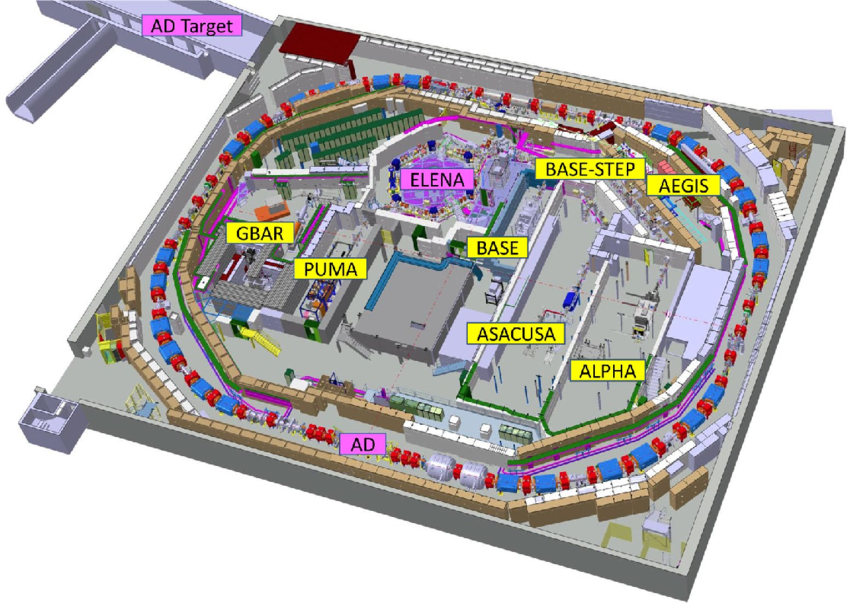
\includegraphics[width = 0.75\textwidth]{figures/chapter 2/Overview-on-the-AD-ELENA-facility-The-AD-with-a-circumference-of-183-m-constrains-the.png}
\caption{Scheme of the Antimatter Factory facility, with the Antiproton decelerator and the ELENA ring. 7 experiments are currently operating, with the ALPHA experimental area on the right side of the diagram.}
\label{fig:ADELENA}
\end{figure}

The historical evolution of the facility is directly reflected in the scientific output of the AD era. Early AD operation enabled the first production of cold antihydrogen (ATHENA and ATRAP, 2002 \cite{Amoretti2002}). Subsequent experiments established trapped-antihydrogen techniques and high-precision spectroscopy (notably in the ALPHA and ASACUSA programs), while complementary Penning-trap measurements (e.g., BASE) provided stringent comparisons of antiproton and proton properties, including charge-to-mass ratio and magnetic moment \cite{Ulmer2015}. In parallel, antiprotonic-atom studies by the ASACUSA collaboration, methodologically connected to the LEAR tradition, continued to contribute to precision bound-state tests. More recently, dedicated experiments (AEgIS, GBAR, ALPHA-g) have extended the scope of the AD program to gravitational observables of neutral antimatter \cite{Aegisproposal}, \cite{GBAR:2011fij} \cite{ALPHA:2013skd}. In this sense, the AD/ELENA complex is not merely a beam-delivery system, but a structured platform that links accelerator performance parameters (energy, emittance, duty cycle, and extraction conditions) to the achievable precision and systematic control of contemporary antimatter measurements.

\section{The ALPHA experiment}

\ALPHA is one of the 7 experiments located at the Antimatter Factory facility at CERN. \ALPHA focuses on antihydrogen physics, and aims to measure energy levels, aiming to perform a comparison with the matter equivalent, as well as gravitational acceleration measurement on antihydrogen. The \ALPHA apparatus, whose schematic overview is shown in Fig.~\ref{fig:AlphaSchematicOv},\begin{sidewaysfigure}[hp]
\centering
\includegraphics[width = \textwidth]{figures/chapter 2/image1.png}
\caption{Schematic overview of the ALPHA apparatus. The antiprotons are received from the antiproton decelerator beam-line, that is connected to the experiment from the left side (Upstream), and collected by the Catching Trap (CT) for plasma manipulation and cooling. The positron plasma comes from a radioactive source from the right side of the image. The two sections of the experiment are clearly visible: the vertical ALPHA-g apparatus, to measure gravitational acceleration on antimatter, and the ALPHA-2 apparatus, designed for spectroscopy. This image is a reproduction from Ref.~\cite{Singh:2025uuo}.}
\label{fig:AlphaSchematicOv}
\end{sidewaysfigure}
is designed to synthesize, by manipulating antiproton and positron plasma, antihydrogen atoms, that are confined by the interaction of the magnetic momentum with an external magnetic field of about \SI{1}{\tesla}. The magnetic field is provided by a superconducting solenoid and several mirror coils. The antihydrogen synthesis is achieved by manipulating antiproton and positrons plasma with a set of Penning--Malmberg traps, which are constituted by electrodes that can be controlled independently, and are used to design electric potential for plasma manipulation. Penning--Malmberg traps are a common tool in non-neutral plasma physics, and are used to manipulate plasmas to obtain the desired characteristics. In \ALPHA three Penning--Malmberg traps are available, that have different purpose: the catching trap (designed for antiprotons capture), the positron accumulator trap (for positron plasma) and the ALPHA2 Penning--Malmberg trap (for antihydrogen synthesis).
 In the following section, a general overview of the experiment section and how antihydrogen is synthesized is presented, with particular focus on the implications for the measurement that is the topic of this thesis.

\section{Penning and Penning--Malmberg traps, physics principles}

A Penning trap confines charged particles using a combination of static electric and magnetic fields \cite{DEHMELT196853,BrownGabrielse:1986geo}. A uniform axial magnetic field  $\vec{B} = B \hat{z}$ provides radial confinement: any transverse motion of a charged particle is bent into a circular orbit by the Lorentz force, preventing radial escape. Axial confinement, which a uniform solenoidal magnetic field alone cannot provide, is instead achieved with a static electric field generated by a set of cylindrical electrodes: the end electrodes are held at a potential of the same sign as the trapped charge, while a central electrode is held at the opposite potential, creating an electrostatic potential well along the trap axis that reflects the particle back toward the centre whenever it approaches either end.

The resulting particle motion is a superposition of three independent oscillations: a fast circular motion in the plane perpendicular to $\vec{B}$, known as the cyclotron motion; a slower axial oscillation along $\hat{z}$ inside the electrostatic well; and a slow azimuthal drift around the trap axis, known as the magnetron motion, arising from the $\vec{E} \times \vec{B}$ drift induced by the radial component of the trapping electric field. In practice, ALPHA traps are cylindrically symmetric, multi-electrode versions of this basic design — Penning--Malmberg traps — in which a stack of many short cylindrical electrodes, rather than just three, allows the trapping potential to be reshaped dynamically along the trap axis, enabling the plasma manipulations (compression, transport, splitting, merging) needed for the experiment \cite{Ahmadi:2018enh}.
Malmberg and deGrassie \cite{PhysRevLett.35.577} extended the single-particle Penning trap concept to the confinement of large numbers of like-charged particles, or non-neutral plasmas, in which collective electrostatic interactions can no longer be neglected. In this regime, the plasma settles into a rigid-rotor equilibrium about the trap axis, with radial confinement governed by the plasma's total angular momentum rather than by single-particle dynamics alone. The practical advantage of a multi-electrode design is that the axial potential can be reshaped purely electronically: by varying the voltages on successive electrodes, a confining well can be deepened, split, merged, or translated along the trap axis, allowing the plasma to be transported and manipulated without ever losing axial confinement. These capabilities make the Penning--Malmberg trap, rather than the single-particle Penning trap, the design of choice for the antiproton and positron plasma manipulations performed throughout the ALPHA apparatus.

\section{The positron accumulator}

The positron accumulator at ALPHA is that part of the apparatus (shown in the upper part of Fig.~\ref{fig:AlphaSchematicOv}) that is designed to accumulate positrons for antihydrogen synthesis. The main mechanism of the apparatus, which is based on cooling/trapping with buffer nitrogen gas, was first designed by Surko and Murphy in 1992 \cite{MurphySurko1992}.
The positrons are provided by a strong radioactive source, which contains $^{22}Na$ sodium, which decays into $^{22}Ne$ through $\beta^{+}$ decay. The isotope has a half-life of 2.6 \textit{y}, which makes it possible to have a stable and reproducible positron plasma for the experimental operation.

Positrons immediately released from the sodium source have energies of the order $keV$, and must be slowed down in order to be trapped and manipulated for antihydrogen synthesis. A fraction of the emitted positrons (the ones emitted with a direction aligned with the accumulator) passes through a solid Neon moderator, which slows positrons down to less than $100 \; eV$ of kinetic energy. Only a fraction of the emitted positrons (efficiency about 1\%) are able to cross the Neon moderator; afterwards they are collected in the positron accumulator volume, a multi-stage device filled with cold low-pressure nitrogen gas (see Fig.~\ref{fig:PositronAccumulator}). Nitrogen acts as a cooling mechanism through elastic collisions (the nitrogen electronic excitation cross-section has a prominent resonance around $9 \; eV$), decreasing positron energies further:

\begin{equation}
e^{+} + N_{2} \rightarrow e^{+} + N^{*}_{2}
\end{equation}

while a Penning--Malmberg trap surrounding the plasma ensures confinement with a potential well. The Penning--Malmberg trap which controls the potential is divided in three stages, and the last allows the application of a \textit{rotating} electric field for plasma size compression \cite{Anderegg:2016rw}. A more detailed description of the design of the positron accumulator and its principles is reported in \cite{10.1063/1.859558} and \cite{10.1063/1.870693}. During normal operation, the accumulations last for \SI{100}{\second}, after which roughly 20 million positrons are accumulated. After the accumulation phase, the buffer nitrogen gas is pumped out to minimize the vacuum contamination along the beam-line, and the positron cloud is moved along the beamline by lowering the potential barrier (see Fig.~\ref{fig:PositronAccumulator}, second panel). Positron plasma transfer along the beam line reduces the available quantity for antihydrogen synthesis to roughly $3.7$ million, which is a target number before the antihydrogen synthesis.

\begin{figure}[!hbtp]
\centering
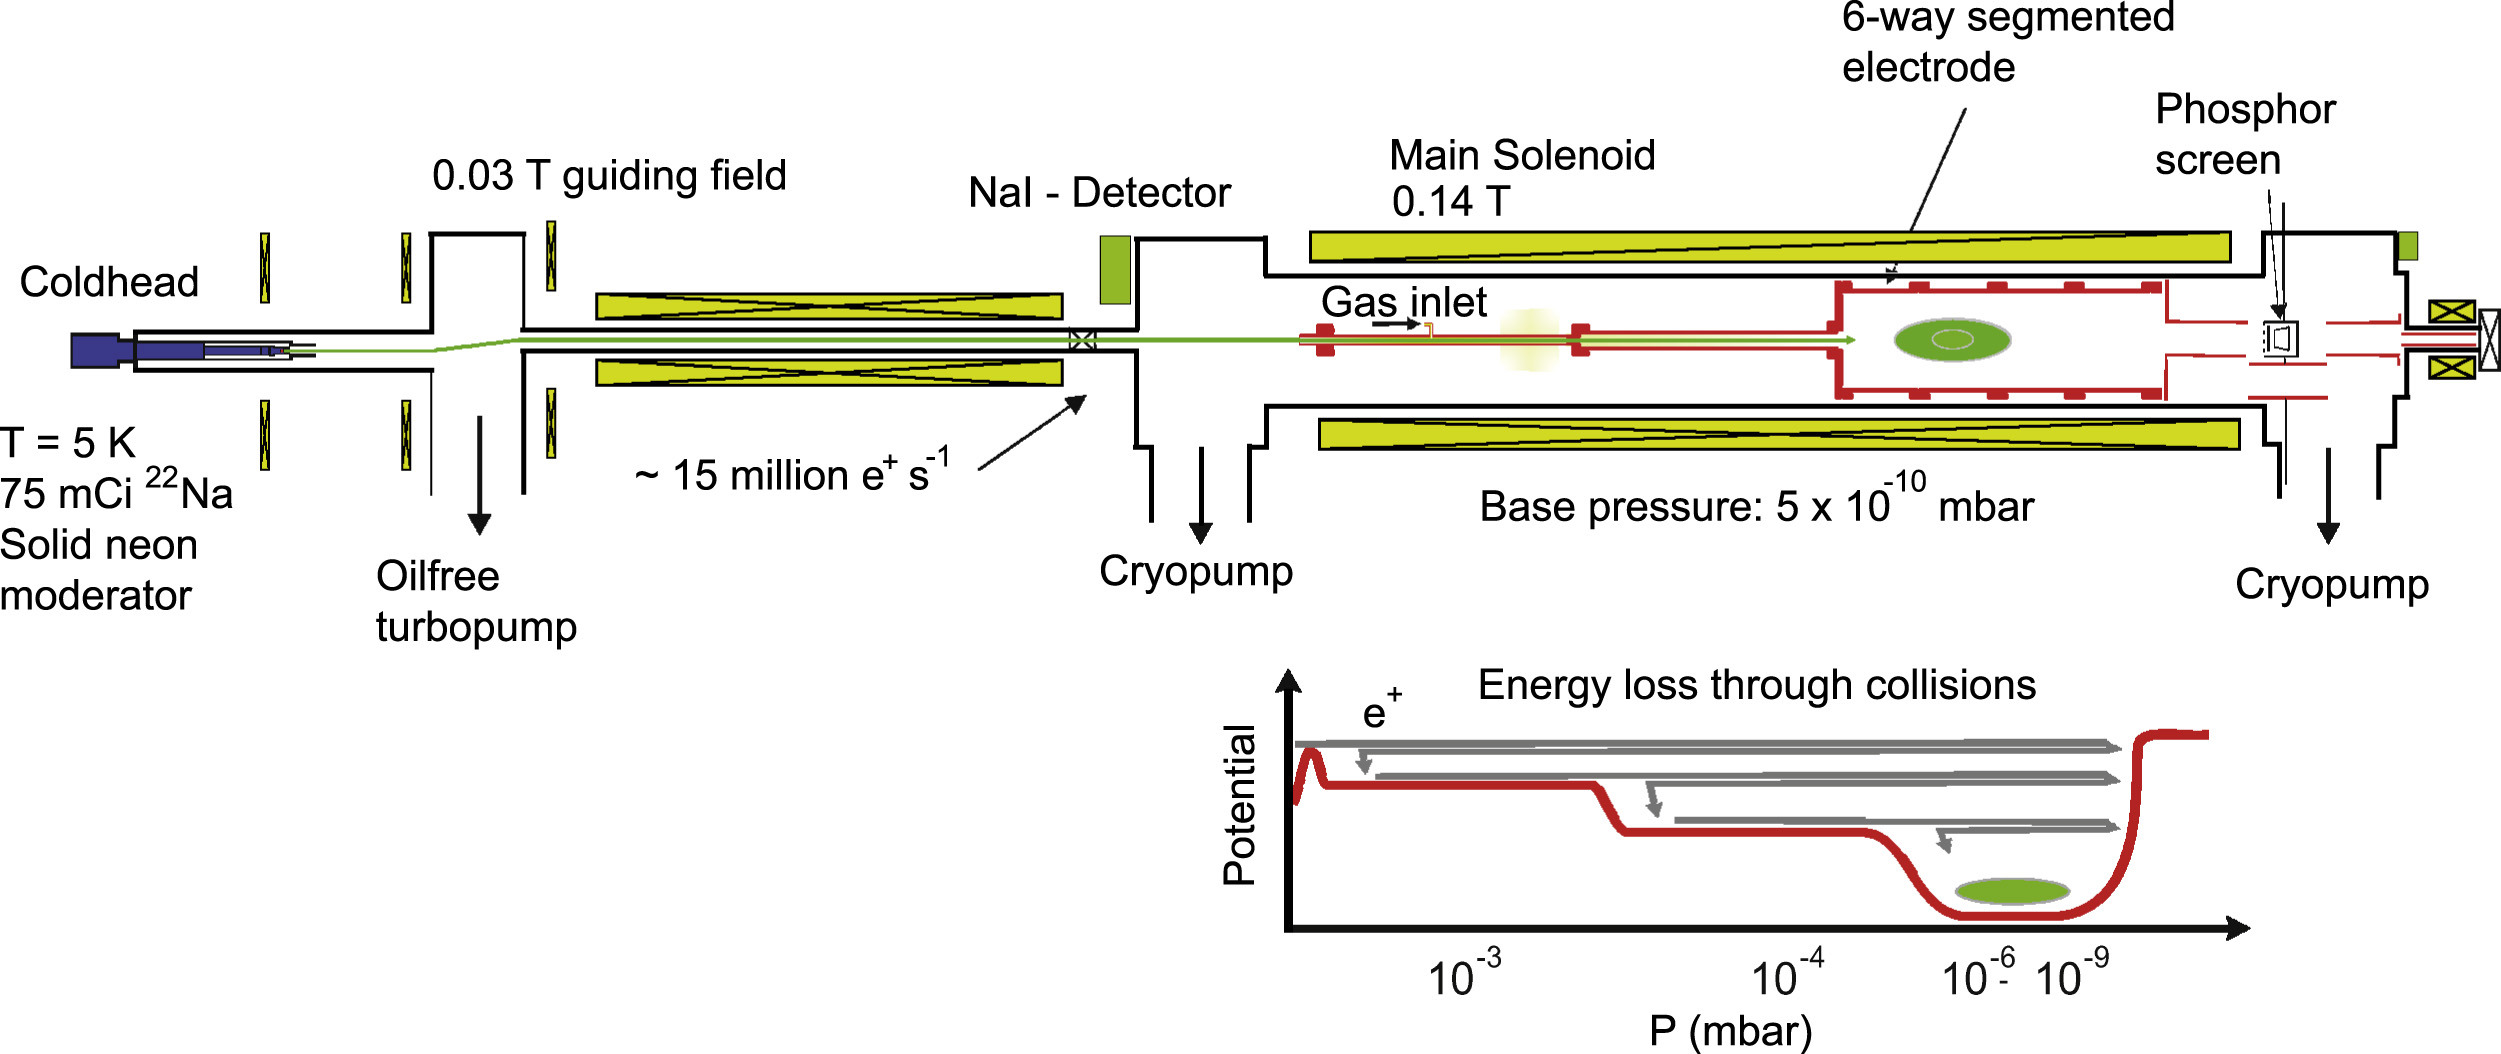
\includegraphics[width = \textwidth]{figures/chapter 2/Positron-acc-scheme.jpg}
\caption{Positron beamline and positron accumulator schematic illustration. The lower panel in the figure represents the axial electric field potential of the Penning--Malmberg trap. The grey arrows represent an example positron trajectory and collisions lead to accumulation of positrons in the third stage of the accumulator volume. The figure is taken from Ref.~\cite{AMOLE2014319}.}
\label{fig:PositronAccumulator}
\end{figure}


\section{The catching trap}

The catching trap (CT) is the device designed for the first stage preparation of antiproton plasma in ALPHA. It receives antiproton bunches from the ELENA ring at a kinetic energy of about \SI{100}{ \kilo \eV}. CT is constituted by a cryogenic Penning--Malmberg trap with a solenoidal field of \SI{3}{\tesla}, located after the ELENA distribution beamline for ALPHA, and it is shown in the left part of the scheme in Fig.~\ref{fig:AlphaSchematicOv} (labeled as \textit{CT}, shown in light green). The antiprotons arriving at the catching trap are first subjected to an energy selection, as they pass through a transverse aluminum foil (degrader) that reduces their kinetic energy \cite{fabbrisiara}. The surviving fraction of antiprotons are captured in the catching trap between two fast-acting high-voltage electrodes. These high-voltage electrodes are energized once the antiproton bunch enters the catching trap volume, in rapid succession raising confining potentials on the ``right'' and ``left'' sides, so that the bunch becomes trapped between them. The potential configuration allows only antiprotons with kinetic energies below $4.5 \; keV$ to remain confined, and the more energetic fraction leaks out.
The antiproton plasma is subjected to several manipulations inside the catching trap. Firstly, the antiprotons are cooled down by using pre-loaded cold electrons in the trap volume. Electrons are useful since they emit Larmor radiation due to their motion inside the trap. The power emitted can be written as:

\begin{equation}
P = \frac{q^{2} a^{2}}{6 \pi \epsilon_{0} c^{3}}
\end{equation}

Here $a$ is the local acceleration experienced by an electron. During their motion inside the trap, electrons tend to emit photons and reduce their available kinetic energy, reaching a much lower temperature with respect to the antiprotons delivered to the experiment. While this cooling mechanism is very efficient for light electrons, it is negligible for antiprotons, since their mass is 2000 times larger\footnote{Assuming a Maxwell-Boltzmann distribution for the charged plasma, it is possible to derive the characteristic cooling time   $\tau = \frac{9 \pi \epsilon_{0} m^{3} c^{3}}{2 q^{4} B^{2}}$, to make explicit the dependence on the mass of the particle species.}. Therefore, antiproton cooling is achieved by elastic collisions with pre-loaded electrons, until the two particle species reach equilibrium at the same temperature.
Sympathetic cooling with electrons typically lasts for \SI{20}{\second}, after which the electrons are removed by quickly lowering and raising the potential well. This procedure, referred to as electron kick (\textit{ekick}), is made fast enough such that very few antiprotons are lost while the majority of the electrons is removed, and it is repeated three times interspersed with cooling periods, leaving a cold antiproton plasma. During the cooling phases, rotating voltages are applied to the segmented electrodes of the trap, so that the mixed antiproton-electron plasma undergoes radial compression, to minimize losses during transfer toward ALPHA-2 (or ALPHA-g) trap.
 Typically, about half a million antiprotons are trapped and cooled with this technique from a single bunch of the \AD, and about $\simeq 350000$ \commento{mmm, quindi però bisogna aggiornarsi rispetto ai mixing triggers, i numeri della tesi di maria non sono aggiornati} are efficiently transferred to the ALPHA-2 left trap (also commonly known as the re-catching trap), where the same cooling mechanism is repeated with another pre-loaded electron plasma. This transfer stage is typically the dominant source of antiproton loss in the whole preparation chain, and ultimately limits the antihydrogen production rate. Once this second cooling stage is completed, the antiproton plasma is placed at the center of the atom trap, for antihydrogen production. 

\section{The ALPHA2 Penning--Malmberg trap}

Until now, the Penning--Malmberg trap has been introduced for the manipulation of charged particles in the experiment. Although such devices are fundamental for charged plasma manipulation and formation of anti-atoms, they cannot be used to trap neutral particles. The ALPHA-2 neutral trap is a hybrid device specifically designed for antihydrogen formation and confinement, that superimposes a Penning--Malmberg trap, used to prepare and manipulate charged antiproton and positron plasma, with an octupole magnet and a series of solenoids. By doing so, it is possible to generate inhomogeneous magnetic field profiles that can exploit the dipole moment of neutral particles or atoms to achieve confinement. 
The ALPHA2 trap is divided in three segments with two different radii. The left and right side traps are made of 7 electrodes of \SI{30}{\milli \meter} each, and are used to ``re-catch'' antiprotons from the catching trap and positrons from the accumulator (the smaller radius allows for larger magnetic field, improving cooling rates). The central, wider trap is made of 13 cylindrical electrodes, with a larger inner radius of \SI{45}{\milli \meter}, and it is instead used for antihydrogen synthesis and confinement. Optical access for the laser system is provided both through off-axis laser ports along the trap and through vacuum windows at the diagnostic stations located at either end of the apparatus.

\begin{figure}[!hbtp]
\centering
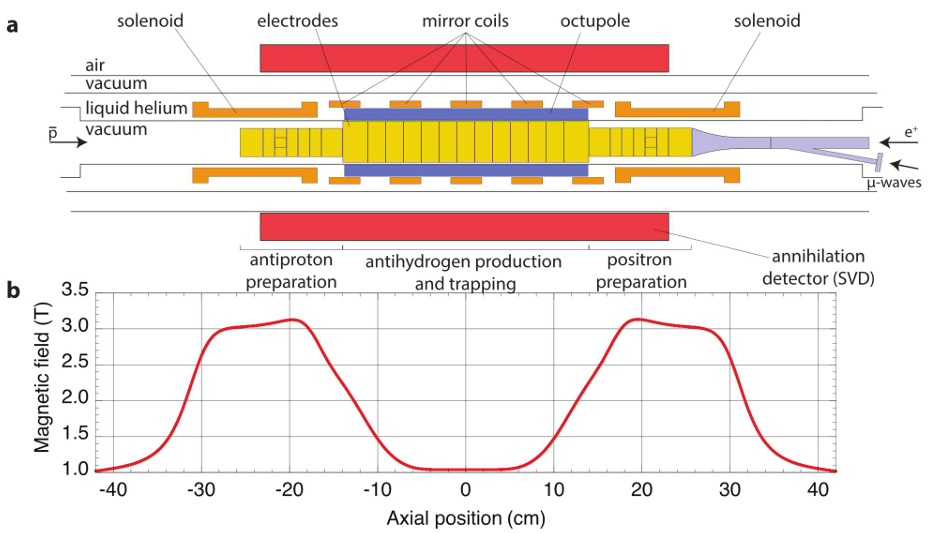
\includegraphics[width=\textwidth]{figures/Bfield_with_tramscheme_draftpaper.png}
\caption{Scheme of the ALPHA2 Penning--Malmberg trap (top) and on-axis magnetic field profile for axial confinement of the antihydrogen atoms (bottom).}
\label{fig:TrapScheme}
\end{figure}

In its ground state, the magnetic moment of antihydrogen originates almost entirely from the positron spin, so that atoms with spin anti-aligned to the local field are drawn towards regions of lower field magnitude (``low-field seekers''), while aligned atoms are repelled. By combining an octupole magnet, chosen over a quadrupole or hexapole configuration to maximize the volume over which the field minimum is flat, with a set of mirror coils providing axial confinement, a local minimum in the magnetic field magnitude is created at the center of the trap. The resulting well has a depth on the order of \SI{0.5}{ \kelvin}, which is dictated by practical magnet current and operational limitations. Only a small fraction of the antihydrogen atoms formed is cold enough to remain trapped. An illustration of the ALPHA2 neutral trap is shown in Fig.~\ref{fig:TrapScheme}. The neutral trap magnetic field is shaped, along the trap axis, like a shallow ``bathtub,'' with a minimum of \SI{1.1}{\tesla} located at the center of the Penning--Malmberg trap (coinciding with the synthesis region) and rising to about \SI{3.3}{\tesla} near the segmented electrodes at either end. This field configuration is produced by superconducting solenoid pairs at each end of the trap (``mirror'' magnets, providing axial confinement) combined with an octupole magnet (providing radial confinement); the octupole is typically operated at 900 A during antihydrogen synthesis. A set of additional mirror coils allows fine adjustment of the field profile to be as axially flat as possible across the synthesis region, maximizing the trapping volume. The preparation and combination of the antiproton and positron plasmas that leads to the actual formation of antihydrogen within this trap is described separately in the following section.


\subsection{Synthesis of antihydrogen} \label{sec:antihydrogensynthesis}

Once the antiproton and positron plasmas have each been individually prepared, cooled, and transferred into the neutral trap (or, in the ALPHA-g apparatus), they are held in separate potential wells until the final stage of the plasma manipulation cycle: mixing. 

The two plasmas are initially located in two smaller potential wells of the Penning--Malmberg trap (left and right side traps) and are moved into the central wider trap. The central trap electrodes produce an electric potential that is designed to both trap antiproton and positron clouds, as shown in Fig.~\ref{fig:Antihydrogen-formation}. The two plasmas are gradually brought closer by lowering the potential barrier between them. Before the barrier is fully removed, the positron plasma undergoes a final evaporative cooling stage, achieved by lowering the potential wall on the side opposite the antiprotons and allowing the most energetic positrons to escape; the remaining positrons re-thermalize at a lower temperature. Then, the potential is further decreased so that antiproton and positron clouds finally merge. This last phase consists of lowering the final separation barrier such that antiprotons are moved into the positron plasma, while positrons are free to escape to the left and get through the antiproton cloud. This mechanism enhances positron evaporative cooling, which acts throughout the mixing phase, lowering the plasma temperature, which ultimately enhances antihydrogen formation.

\begin{figure}[hbtp]
\centering
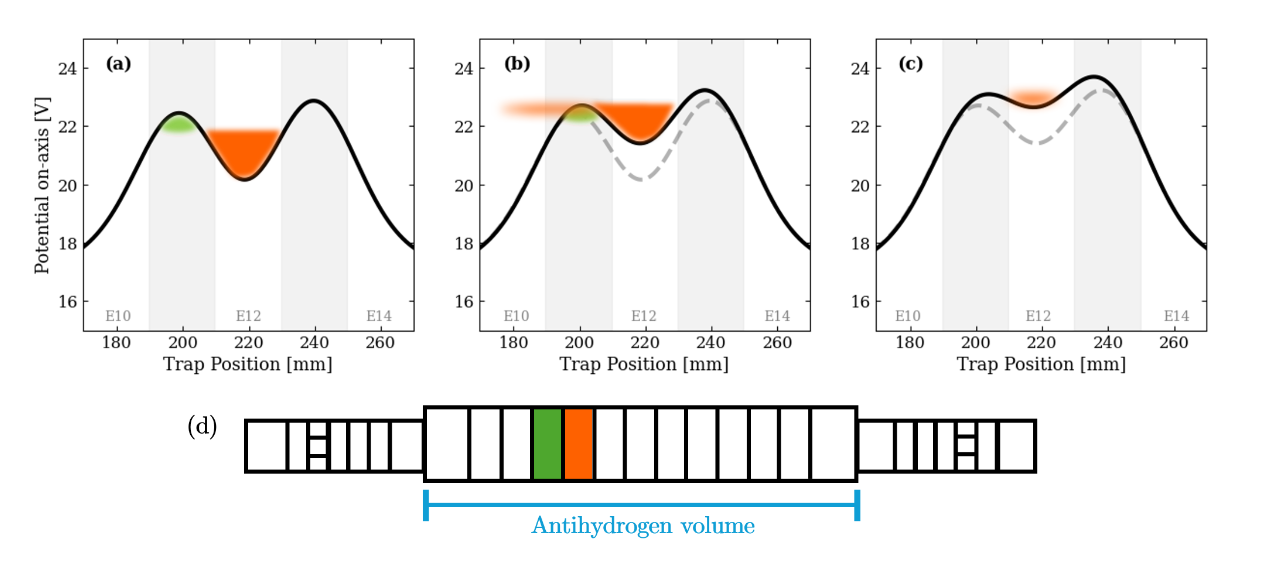
\includegraphics[width = \textwidth]{figures/chapter 2/Antihydrogen_formation.png}
\caption{ This picture illustrates the slow merge technique used to synthesize antihydrogen. Positron (orange cloud) and antiproton plasma (green cloud) are initially in separate locations as shown in \textbf{(a)}. By slowly raising the central potential minimum, antiproton and positron clouds meet, and antihydrogen is synthesized through three-body recombination \textbf{(b)}. The mixing phase ends with the final potential state shown in \textbf{(c)}, with some positrons still trapped, and used for diagnostic purposes (i.e., to measure the final positron temperature after mixing). The duration of the mixing phase is typically in the range of a few seconds, and it is a parameter tuned to maximize antihydrogen production. This figure is reproduced from \cite{goncalves:2025uuo}.}
\label{fig:Antihydrogen-formation}
\end{figure}

Antihydrogen is formed by a three-body recombination process \cite{GlinskyONeil:1991gca}. The process consists of two positrons simultaneously getting close to an antiproton: one positron binds with the antiproton and forms antihydrogen, while the other is ejected away carrying the excess energy:

\begin{equation}
\overline{p} + e^{+} + e^{+} \rightarrow \overline{H} + e^{+}
\end{equation}

This channel is favored compared to two-body recombination. The reason is that for the two-body recombination process, the kinetic energy of the formed anti-atom is comparable to that of the antiproton participating in the process. The resulting kinetic energy of the anti-atom is comparable to the thermal energy of the antiprotons, which makes it difficult for the atom to be cold enough to be confined by the magnetic field minimum (of the order of \SI{0.5}{\kelvin}). Three-body recombination, by contrast, can in principle produce antihydrogen without depositing this excess energy into the atom's kinetic energy, making it the dominant source of trappable atoms under ALPHA's experimental conditions. Of all antihydrogen atoms formed during a mixing cycle, only the fraction with kinetic energy below the trap depth remains confined once the mixing sequence ends; the rest escape and annihilate on the surrounding electrode walls. At the end of the mixing, the magnets can be de-energized, to release confined antihydrogen, or kept energized while other mixing cycles are performed in succession, in order to accumulate a larger sample of anti-atoms (stacking technique).

\subsection{Beryllium cooling}

The Beryllium cooling system constitutes a fundamental milestone for the \ALPHA experiment, since it has improved antihydrogen formation from a few atoms to hundreds of atoms, also reducing the final antihydrogen temperature distribution. This technique has been established in \ALPHA in 2024, and it is extensively described in Maria Gomes Goncalves's thesis \cite{goncalves:2025uuo}, and results were published in Nature Communications (\cite{Baker:2021ink}). During the 2024/2025 experimental campaign, further improvements of the Beryllium cooling system allowed a record accumulation of over 15000 trapped antihydrogen atoms in 7 hours \cite{Akbari:2025mli}.

A well-established solution in non-neutral plasma physics is sympathetic cooling: a species that can be cooled directly (the coolant), typically via laser cooling \cite{Wineland:1978rpc}, is mixed with the species to be cooled (the target), and energy is transferred between the two populations through Coulomb collisions. This approach was first demonstrated in 1986 by cooling $^{198}Hg^{+}$ ions through collisions with laser-cooled $^{9}\text{Be}^{+}$ in a Penning trap \cite{Larson:1986sc}, and its use to cool positron plasmas via laser-cooled $Be^{+}$ ions was subsequently demonstrated in 2003 \cite{Jelenkovic:2003pos}. At ALPHA, this technique has been extended to routinely cool millions of positrons to cryogenic temperatures directly within the Penning--Malmberg trap used for antihydrogen production.

$^{9}\text{Be}^{+}$ is selected as a coolant species because it is the lightest ion with an electronic structure suitable for direct laser cooling, minimizing the mass ratio between the target species and the coolant, which maximizes the energy exchange through collisions.

The $\text{Be}^{+}$ ions are produced in situ by pulsed laser ablation of a solid beryllium target — a method chosen for its compatibility with the geometry and vacuum requirements of the cryogenic trap, avoiding the need for an external atomic beam source — and are then laser-cooled on a cycling optical transition (wavelength \SI{313}{\nano \meter}) before being merged with the positron plasma. As cooling proceeds, Coulomb collisions transfer energy from the positrons to the colder $\text{Be}^+$ ions; however, as the plasma cools, the heavier ions migrate radially outward relative to the positrons due to centrifugal separation \cite{ONeil:1981cent}, reducing the spatial overlap between the two species and eventually limiting the minimum achievable positron temperature to a few kelvin, well above the Doppler limit of the $\text{Be}$ ions themselves. This limiting temperature depends on the number of ions used, initially decreasing with a larger coolant population before plateauing once centrifugal separation sets in \cite{Andresen:2011cent}.

This ``Final Laser Cooling'' step, performed immediately before mixing, has become the standard technique for preparing cold positron plasmas at ALPHA, replacing purely evaporative cooling schemes. The resulting increase in positron phase-space density has translated into a substantially higher antihydrogen yield, with $\text{Be}^{+}$ assisted cooling reported to increase the number of trapped antihydrogen atoms per synthesis cycle by roughly a factor $\approx 10$ between the 2023 and 2024 experimental runs.

\subsection{Laser cooling of antihydrogen} \label{sec:lasercooling}

Once trapped, the antihydrogen atoms retain a kinetic energy comparable to the depth of the neutral trap, of the order of \SI{0.5}{\kelvin}. Since the density of the trapped sample is too low for collisions to redistribute energy, evaporative cooling, as used for charged plasmas, cannot be applied, and laser cooling is the most practical way to further reduce the energy of the anti-atoms \cite{Evans:2022thesis}. In 2021, \ALPHA demonstrated the first laser cooling of trapped antihydrogen \cite{Baker:2021ncj}.

The technique relies on Doppler cooling. A laser beam is tuned slightly below (red-detuned) the frequency of an atomic transition, so that, because of the Doppler effect, it is preferentially absorbed by atoms moving towards the source. Each absorbed photon transfers a momentum $\hbar k$ opposite to the atomic velocity, while the subsequent spontaneous emission occurs in a random direction and averages to zero over many absorption-emission cycles. The net effect is a velocity-dependent friction force, which is maximal for a detuning of about half the natural linewidth $\Gamma$ of the transition \cite{Evans:2022thesis}. The lowest temperature reachable by this process is the Doppler limit,

\begin{equation}
T_{D} = \frac{\hbar \Gamma}{2 k_{B}},
\end{equation}

set by the balance between cooling and the heating from the random recoils of the emitted photons.

For (anti)hydrogen, the cooling transition is the Lyman-$\alpha$ line (1S-2P) at \SI{121.6}{\nano\meter}, with a natural linewidth $\Gamma/2\pi \approx \SI{100}{\mega\hertz}$, which gives $T_{D} \approx \SI{2.4}{\milli\kelvin}$; because of the small mass of the atom and the high photon energy, the single-photon recoil temperature ($\approx \SI{1.3}{\milli\kelvin}$) is comparable to the Doppler limit, unlike in the alkali atoms commonly used in laser cooling experiments \cite{Evans:2022thesis}. In \ALPHA, the cooling light is produced by a pulsed laser system: a \SI{730}{\nano\meter} continuous-wave seed laser is amplified in a pulsed cavity, frequency-doubled to \SI{365}{\nano\meter}, and finally tripled to \SI{121}{\nano\meter} by third-harmonic generation in a krypton-argon gas cell, producing pulses of about \SI{10}{\nano\second} at a repetition rate of \SI{10}{\hertz}, with energies of the order of \si{\nano\joule} in the trap \cite{Evans:2022thesis}. The laser is tuned to the transition between the trapped $\ket{d}$ ground state and the $2P$ state with the highest energy in the magnetic field (labelled $2P_f$), which ensures that the excited atoms decay back to the same trapped state and can repeat the cycle \cite{Baker:2021ncj,Evans:2022thesis}.

The laser beam enters the trap almost parallel to its axis (at an angle of about \SI{2.2}{\degree}), so that the cooling force acts directly only on the axial motion. Nevertheless, the anharmonicity of the magnetic trap couples the axial and transverse degrees of freedom of the atomic orbits, so that the energy of the whole three-dimensional motion is reduced \cite{Evans:2022thesis}. The cooling effect was observed both as a narrowing of the Doppler-broadened 1S-2P line, sensitive to the velocity along the beam, and as a narrowing of the Doppler-free 1S-2S line, whose width is dominated by transit-time broadening and is thus sensitive to the transverse velocity. The mean kinetic energy of the sample was reduced by about an order of magnitude, down to a few tens of \si{\milli\kelvin} \cite{Baker:2021ncj,Evans:2022thesis}. The final temperature remains well above the Doppler limit, since the absence of collisions between the anti-atoms strongly limits the rate at which energy is redistributed among the degrees of freedom and removed \cite{Evans:2022thesis}; nevertheless, colder samples reduce the linewidths in laser spectroscopy and are a key ingredient for future precision measurements with antihydrogen \cite{Evans:2022thesis}.

\section{Electron cyclotron resonance technique (ECR)} \label{sec:ECRtecnique}

The ECR (Electron Cyclotron Resonance) is a powerful sensing technique, developed in the \ALPHA collaboration, to measure the on-axis magnetic field in a Penning--Malmberg trap. This technique has been developed in 2014 \cite{Amole:2014lna} and refined by \textit{Eric Hunter} \cite{Hunter_2020}, and exploits the interaction between a small electron plasma and the external magnetic field, combined with microwave radiation injected into the trap, to determine the magnetic field magnitude at a given axial position. Accurate measurements of the magnetic field are required for precision measurements of the atomic spectra as well as the gravitational acceleration of antihydrogen in ALPHA-g.

The measurement relies on a Penning--Malmberg trap, in which a large electron plasma reservoir ($2$--$3\times10^{7}$ electrons) is first prepared and stabilized in temperature, density and particle number via strong-drive regime evaporative cooling (SDREVC). Small target plasmas, containing as few as $N_T \sim 1500$ electrons, are then repeatedly extracted from the reservoir by manipulating the electrode potentials, moved to a dedicated heating well, and further evaporatively cooled (see Fig.~\ref{fig:SchemeECR}). This reservoir-based approach allows more than 100 target plasmas to be produced from a single loading of the electron source, enabling a complete frequency scan in about one minute and avoiding the systematic drifts associated with repeated source operation.
Assuming the z parallel to the trap axis, each target plasma is moved along the axis to the location of interest by tuning the electrode potentials. Then, the plasma is kept in place by the electrode potential (also experiencing a magnetic field $B\hat{z}$) and it is illuminated with a microwave pulse (typically $100\,\mathrm{ms}$ long) whose frequency $F$ is swept across a range of values. When $F$ approaches the electron cyclotron frequency $f_c = eB/2\pi m_e$, the plasma absorbs energy from the microwave field and is heated. The resulting plasma temperature is measured destructively: the downstream confinement potential is slowly lowered at a fixed rate, and the arrival rate of the escaping electrons at a microchannel plate (MCP) detector is recorded. Since the most energetic electrons escape first as the barrier is lowered, the time history of the MCP signal directly encodes the plasma temperature, which is extracted through a fit to the expected escape-rate model.

A frequency scan typically reveals not a single resonance but a series of heating peaks, spaced by the electron axial bounce frequency $f_z$ and further split into subpeaks separated by the plasma (magnetron) rotation frequency $f_r$. These sidebands arise because the oscillating electron motion in the trapping well and its slow rotation around the trap axis modulate the microwave field seen by the electron, shifting the resonance condition away from the bare cyclotron frequency. Among these substructures, the $l=-2$ subpeak of the central ($m=0$) resonance is identified as the one whose frequency is, to first order, independent of both the bounce and rotation frequencies, and is therefore taken as the true cyclotron resonance used to extract $B$ through inversion of $B = (2\pi m_e/e)\,f_c$.
The origin of the bounce sidebands can be understood simply: while bouncing back and forth along the trap axis, an electron crosses regions where the amplitude and phase of the microwave field are different, so that in its own frame the field is modulated at the bounce frequency, and absorption also occurs at $f_c \pm f_z$ and at its harmonics. The sidebands are clearly visible in relatively shallow wells ($f_z \lesssim \SI{10}{\mega\hertz}$), while in deeper wells they become smaller and move further away from the main peak \cite{HunterThesis2019}. Since $f_z$ is set by the depth and shape of the confining well, while $f_c$ depends only on the magnetic field, the sidebands move when the well is changed, whereas the central peak stays at the same frequency. In the same way, changing the length of the well changes the rotation frequency $f_r$ and moves the rotation subpeaks, while the $l=-2$ subpeak of the central resonance does not move. Repeating the scan with wells of different depth and length is therefore a simple way to identify the peak corresponding to the cyclotron frequency; the same check also allows spurious heating of the reservoir plasma, which sits at a different field, to be distinguished from the response of the target plasma \cite{HunterThesis2019}.

Using this method, ALPHA reports absolute magnetic field measurements with an accuracy better than $1\,\mathrm{ppm}$, and a relative precision of $26\,\mathrm{ppb}$ when combining several bounce-frequency scans, dominated respectively by environmental field drifts (of thermal origin, linked to the electron source) and by residual plasma-charge and finite-temperature systematic shifts.

\begin{figure}[hbtp]
\centering
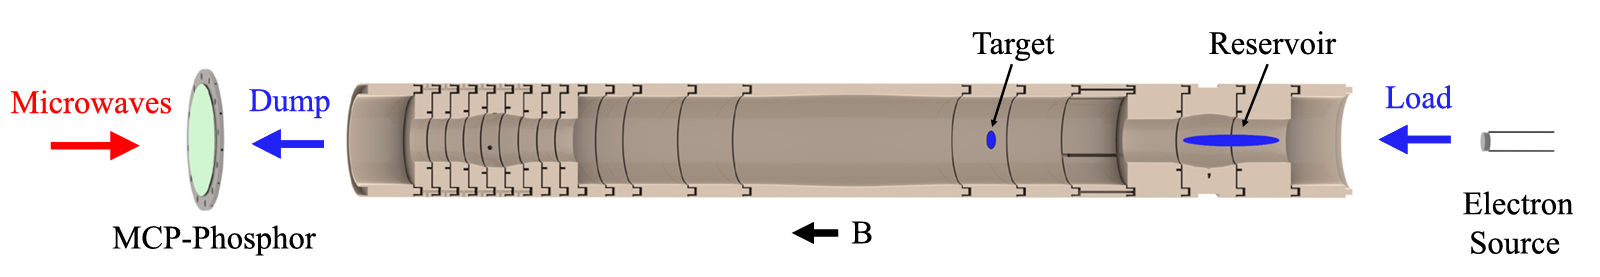
\includegraphics[width=\textwidth]{figures/chapter 2/ECR-scheme.png}
\caption{Scheme of ALPHA-2 Penning--Malmberg Trap, with illustration of the main ECR measurement phases (preparation of the plasma reservoir, extraction, microwave heating and dump). The figure is reproduced from Ref.~\cite{Hunter_2020}.}
\label{fig:SchemeECR}
\end{figure}

The ECR technique is actually used in the measurement both for designing the magnetic trapping potential for synthesis of antihydrogen and spectroscopy in ALPHA-2, and furthermore makes it possible to keep track of magnetic field changes by repeating ECR measurements in a time series.


\section{Detection of antiprotons}

The detection of antimatter in the ALPHA2 experiment is made possible with a silicon vertex detector (SVD), designed for annihilations once an antihydrogen atom or an antiproton hits the electrodes of the trap. The annihilation products are mainly charged pions $\pi^{\pm}$, and by reconstructing and analyzing the tracks of their passage in the detector, it is possible to extract the vertex of the annihilation, which is the main measurement tool in spectroscopy experiments \cite{ALPHA:2012wlk}.
The detector consists of three concentric layers of double-sided silicon microstrip modules, arranged coaxially around the trap magnets so as to surround the entire synthesis region. The annihilation products are mainly charged pions $\pi^{\pm}$, and by reconstructing and analyzing the tracks left by their passage through the successive silicon layers, it is possible to extract both the spatial position and the timing of the annihilation vertex, with a typical resolution of about 0.5 cm along the trap axis and 0.9 cm radially \cite{Capra:2015ozr}. This vertex reconstruction is the main measurement tool in spectroscopy experiments, and it also allows genuine antiproton annihilations to be distinguished from a background of cosmic-ray events, based on the track topology and timing of the reconstructed events.

\subsection{Imaging detector: the silicon vertex detector}

The silicon vertex detector is a 3-layer detector that is placed around the trap center reaching almost full azimuthal coverage. The scheme of the detector is shown in Fig.~\ref{fig:SVDscheme}. The detector is made of 72 modules, each constituted by 256 p-side and 256 n-side strips. The modules are arranged in two separate halves along the axial direction, each consisting of 36 modules distributed over three concentric layers. The choice of a multi-layer detector is driven by the fact that in such a way it is possible to sample three points of the trajectory of a charged pion in its flight, and hence reconstruct the track of the particle, and the annihilation vertex.

Each module (also called hybrid) consists of two double-sided silicon sensors, \SI{300}{\micro\meter} thick, each with an active area of $5.8 \times \SI{11.2}{\centi\meter\squared}$, mounted on a \SI{1.6}{\milli\meter} thick printed circuit board; the two sensors are bonded together along the p-strips, which run parallel to the trap axis, so that each module covers about \SI{22}{\centi\meter} along the axis. The p-strip pitch is \SI{227}{\micro\meter} and the n-strip pitch \SI{875}{\micro\meter} \cite{Capra:2015ozr}. In each of the two halves, placed on either side of the trap center, the inner, middle and outer layers consist of 10, 12 and 14 modules, respectively. The modules of each layer are staggered in radius to improve the solid-angle coverage, and are located at radii of \SIlist{8.90;9.45}{\centi\meter} (inner layer), \SIlist{10.80;11.35}{\centi\meter} (middle layer) and \SIlist{12.70;13.25}{\centi\meter} (outer layer) \cite{Capra:2015ozr}. The detector is constrained in radius by the outer diameter of the beam pipe (\SI{16}{\centi\meter}) and by the inner bore of the external solenoid (\SI{35}{\centi\meter}), and has a total of \num{36864} readout channels \cite{Capra:2015ozr}.

\begin{figure}[hbtp]
\centering
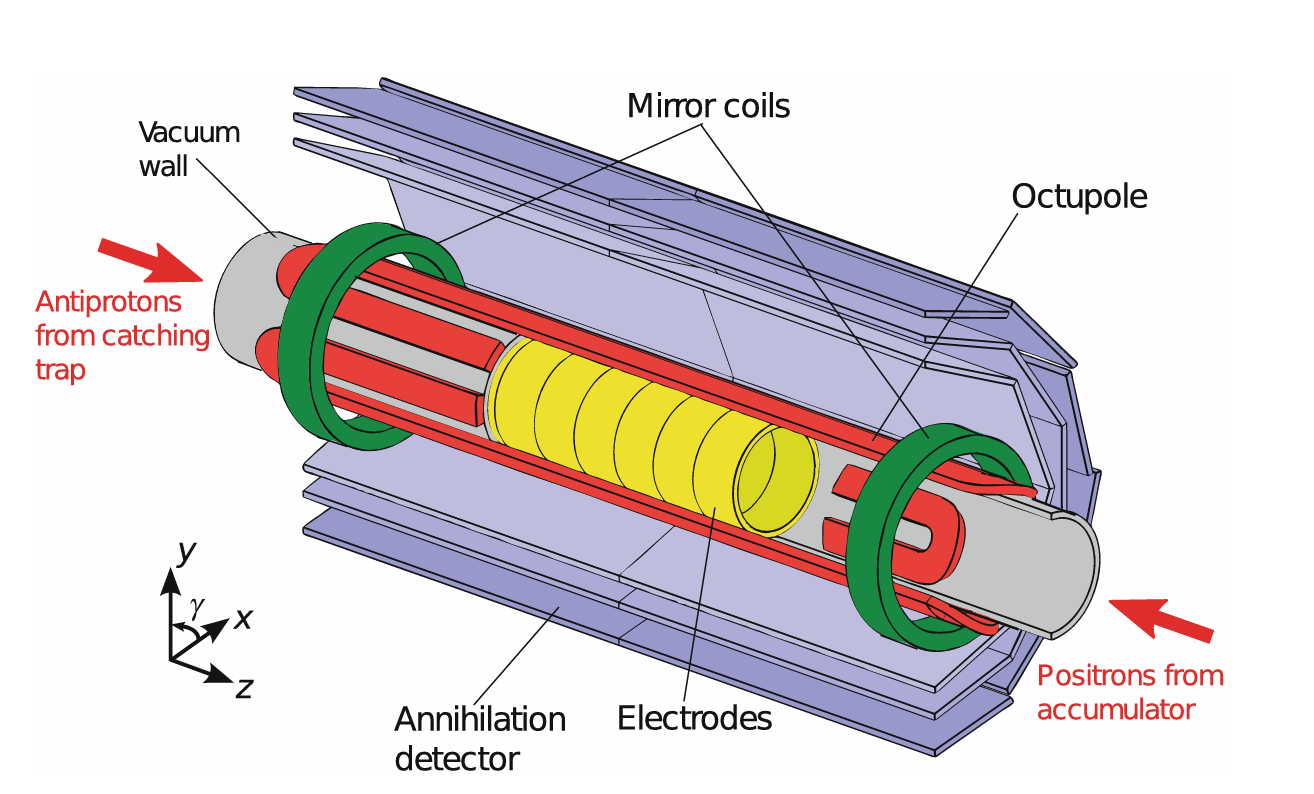
\includegraphics[width = 0.75\textwidth]{figures/chapter 2/Alpha2 Detecor.png}
\caption{Scheme of the ALPHA2 silicon vertex detector (not to scale). The detector is made of 72 modules, that are read out by ASICs. The figure is reproduced from \cite{ALPHA:2012wlk}.} \label{fig:SVDscheme}
\end{figure}

The signals of the detector are constituted by `hits' in the silicon strips of each module, that are read-out by VA1TA ASIC read-out chips, which control both the read-out and the trigger of an acquisition.
The position information of a hit within a module is achieved by combining the signal information of the p-side and n-side strips of a \textit{hit}, and the passage is localized in the plane of the module (see Fig.~\ref{fig:SVDtrack}).

\begin{figure}[hbtp]
\centering
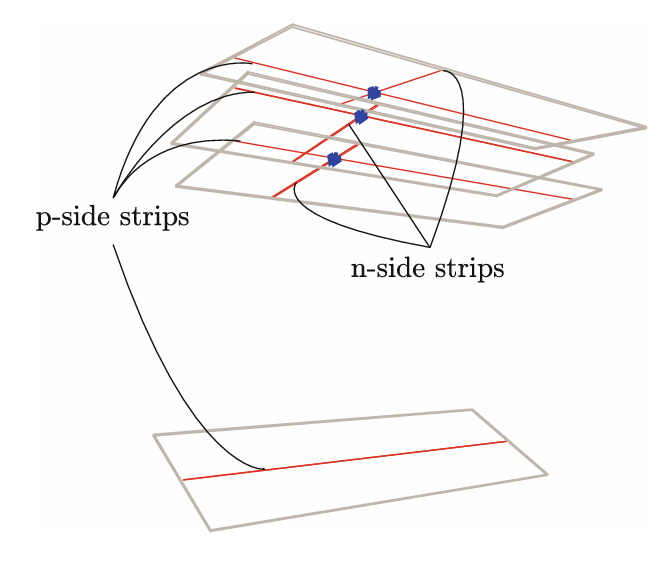
\includegraphics[width = 0.75\textwidth]{figures/chapter 2/Example-of-track.png}
\caption{Example of track and localization of the position of the passage within a module of the detector. The image is reproduced from \cite{Hydomako2013}.}
\label{fig:SVDtrack}
\end{figure}

During an experiment, the main source of background is constituted by cosmic tracks, mainly charged cosmic muons $\mu^{\pm}$, that are recorded by the detector. These energetic cosmic muons travel across the apparatus and are recorded as a single track composed of six hits. The topology of the cosmic events is different from the ones coming from real antiproton or antihydrogen annihilation, hence various pieces of information can be used to discriminate the two cases. This information is combined in a Multi-Variable Analysis (MVA) that is used to effectively suppress the cosmic background.

\section{External scintillators}
\contentof{Qui si può parlare un po' dei burritos, perchè no, come progetto collaterale}

The previous section briefly described the main detector used for antihydrogen detection. \ALPHA has several detectors which are used for imaging the plasma or measuring its temperature, etc.
The \ALPHA experiment apparatus is provided with different diagnostic stations, some of which are highlighted in Fig.~\ref{fig:AlphaSchematicOv} with blue arrows, which are equipped with Microchannel plates made with phosphor (also known by the abbreviation MCP) \cite{Andresen:2009mcp}. The MCP is a two-dimensional detector that can detect electrons, ions, X-rays in vacuum, and it is a common tool in plasma physics. When a charged particle traverses the MCP, it produces a cascade of secondary electrons that produce phosphorescence photons, which are collected by a CCD camera, producing an image of the plasma in the \textit{x,y} plane of the MCP plate. These diagnostic stations are widely used in \ALPHA to study the temperature, size and evolution of the various plasmas (electrons, positrons, antiprotons) along the beamline. They provide good spatial resolution, which allows them to be used for alignment and to benchmark several plasma manipulation techniques. However, although providing spatial information, it is hard to use such detectors to characterize the time structure of the plasma dump when moved along the beamline. In light of this, part of the work of this thesis was dedicated to the development of a system of fast scintillators, placed at several locations along the apparatus, to measure the time distribution of the positron plasma during the various transfers along the trap. The choice of the detector has been made considering that the width of the positron plasma (in terms of time distribution) is expected to be on the order of $\approx$ \SI{10}{\nano \second}, which requires fast detection, namely a detection mechanism that is fast enough so as not to cause signal smearing that would result in a loss of information. Another collateral consideration was driven by the fact that the environment in the proximity of the beamline and of the various Penning--Malmberg traps is influenced by magnetic fields that are not shielded. The natural choice was to employ plastic scintillators coupled with silicon photo-multiplier devices. The scintillating material used for this application is the Ej-200, a plastic scintillator made with polyvinyltoluene doped with fluorophores \cite{eljensite}. The scintillating material was selected for being sensitive to gamma rays emitted by positrons, once they annihilate on the plate of an MCP, or on the beamline frame in case of losses. The gamma rays are converted into visible light (blue light $\approx$ \SI{425}{\nano \meter}) that is detectable by SIPMs that are connected via an optical coupler to one side of the scintillating material. The signal produced by the SIPMs is then processed with an OPA354 signal amplifier, in TIA mode (so converting the current signal from the SIPM to a voltage signal). The signal output is still analog, and it is sent to Red Pitaya FPGA boards, that are used as the DAQ system. Each Red Pitaya has two input channels, that can acquire independently two signals with a minimum sampling rate of \SI{8}{\nano \second} and a buffer length of 16384, corresponding to a time span of \SI{131.072}{\micro \second}. The Red Pitayas are controlled by an online Python script that continuously monitors the devices, triggers new acquisitions, and saves the data in \textit{.txt} format for further analysis. A separate Python script takes care of analyzing the signals once they are collected, running continuously. The analysis of the signals consists first of a de-noising procedure, where spurious noise is eliminated by applying a low-pass filter with a \SI{9.3}{\mega \hertz} cutoff; hence the offset of the signals is subtracted, and the signal is fitted with an asymmetric Gaussian function, to extract the FWHM, the peak time position, the amplitude and the total area of the signal (which is proportional to the total number of positrons). This information is then recorded on CERN \textit{EOS}, which is a distributed storage system available at CERN. Together with Dr. Samuel Niang, who is responsible of the positron accumulator in \ALPHA a web application has been implemented, through which operators can visualize, during the daily experimental routine, signal plots produced by the analysis program. The provided informations are used to steer positron during the design of new experimental protocol, to increase the number of captured positrons, identify losses during transfer between sections, and are also helpful to decrease the bunch size of the positron plasma. The web application was implemented using the \textit{NGINX} library, and it is accessible from the CERN local network. An example of dump recorded and shown in the web application is in Fig. \ref{fig:Burrito-webint-1}

\begin{figure}[hbtp]
\centering
\includegraphics[width=\textwidth]{figures/chapter 2/ALPHA Burrito Detectors.pdf}
\caption{Web interface of the fast scintillation detector system. The web interface is called \textit{ALPHA Burrito Detectors}, following an internal slang of the collaboration. From the web interface it is possible to select the range of the plots, check the status of the analysis and acquisition scripts as well as the temperature of the FPGA in the \textit{redPitaya} boards (diagnostic). The detectors are sorted depending on their location along the beam-line, and several parameters from the fit are reported in a separate table. A skimmer is also present, that generates list of analysis output organized by acquisition. These outputs are typically used to monitor stability or parameter variations based on machine settings.} \label{fig:Burrito-webint-1}
\end{figure}





\chapter{Hyperfine splitting of the antihydrogen ground state}
\label{ch:hyperfine}
\contentof{This chapter recalls a bit of theory about the energy levels of antihydrogen and focuses on the lines that have been measured at ALPHA. Important to mention the zeeman broadening, since we are working at non-zero field, and the experimental protocol of the measurement. Things to mention are ECR, microwave hardware, magnetic field map. Then a description of the experimental protocol, magnetic field decay}

The hyperfine structure is defined as a small shift (roughly 2000 times smaller than that relative to the fine structure) in the energy level of atoms and molecules. This shift originates from the electromagnetic interaction of the electron magnetic momentum and the magnetic/electric multipole moment of the nucleus. Although the shift is smaller compared to the magnitude of the energy level gap and other effects, such as the fine structure of the atoms, it is of great interest in atomic physics and astrophysics as well as in antimatter studies. From the atomic physics point of view, the transition between the 1S hyperfine levels of hydrogen is an important quantity, that has been measured with a remarkable precision of \SI{2}{\milli \hertz} (\cite{bestHFShydrogen}), corresponding to a relative precision of \num{1.4e-12}. In nuclear physics, transitions between hyperfine energy levels offer the possibility of investigating the internal structure of the proton and other nuclei and provide a test of QED \cite{Karshenboim:2005iy}. From the astrophysical point of view, the 1S hyperfine splitting corresponds to the \SI{21}{\centi \meter} line, which is transparent to the galactic medium and has been extensively used to map hydrogen density of galaxies, galaxy rotation curves, redshift effect \cite{Dickeyarticle} and to test variation of fundamental constants (fine structure constant and g factor of the proton) over time \cite{Khatri_2007}. In the antimatter field, this spectral line can be used to test CPT symmetry, by repeating the same measurement on antihydrogen. Currently, two experiments at the antimatter factory at CERN have the capability to perform this measurement as part of their physics programs: the ASACUSA collaboration \cite{Diermaier:2016fsy}, that aims to measure the hyperfine splitting on an antihydrogen beam (on-flight measurement) and the ALPHA collaboration, that demonstrated in 2012 of being able to induce quantum transition on trapped antihydrogen atoms \cite{ALPHA:2012kaf}. This technique was relying on the usage of microwave light injected into the trap volume, that led a few years later, in 2017, to the first measurement of the ground state hyperfine splitting \cite{ALPHA:2017fsh}. The most recent measurement \cite{ALPHA:2026lbu}, the topic of this thesis, has improved by a factor 100 the final uncertainty.
The present chapter will give an introduction to the physics underlying the measurement and outline the experimental protocol followed in 2023/2024, that has improved the uncertainty by a factor $\simeq$ 50.
The following derivation follows the approach in the book \cite{QuantumMechanics}. Only the case of the hyperfine level of the ground state, which is of particular relevance to this thesis, will be discussed; certain details will be omitted, so as not to burden the discussion.

\section{Hyperfine structure}
\contentof{This section can contains a brief derivation of the physics behind the hyperfine levels of antihydrogen. Present a brief derivation of the physics}

The antihydrogen atom is a bound state of a positron and an antiproton. The base Hamiltonian of this system, neglecting all higher-order terms, takes the form of $H_0 = \frac{p^2}{2\mu} + V(r)$ where $\mu$ is the reduced mass of the antiproton/positron system, and $V(r)$ is the central static electromagnetic potential. When considering relativistic effects, several higher-order terms appear, which are encompassed in the equation\footnote{In the full Hamiltonian, $\mu = m_e$ has been used, assuming infinite mass for the antiproton}:

\begin{equation}
H = m_{e} c^2 + \frac{p^2}{2m_e} + V(r) - \dfrac{p^4}{8 m_{e}^3 c^2} + \frac{1}{2m_{e}^2 c^2} \dfrac{dV(r)}{r dr} L \cdot S + \frac{\hbar^2}{8m_{e}^2 c^2} \Delta V(r) + W_{hf} + ...
\end{equation}

The content of this full Hamiltonian can be summarized as:

\begin{itemize}
\item $- \dfrac{p^4}{8 m_{e}^3 c^2}$ corresponds to the first relativistic energy correction, and can be easily obtained by expanding in series the relativistic energy $E = c \sqrt{p^2 + m_{e}^{2} c^2}$;
\item $+ \frac{1}{2m_{e}^2 c^2} \dfrac{dV(r)}{r dr} L \cdot S$ this is the term responsible for the fine structure of the atoms, and corresponds to the coupling of the positron magnetic moment ($M_s = \frac{q S}{m_{e}}$) with its angular momentum $L$ (spin-orbit interaction);
\item  $\frac{\hbar^2}{8m_{e}^2 c^2} \Delta V(r)$ is the Darwin term, that arises when we consider non-local interaction between the electron and the Coulomb field of the nucleus;
\item $W_{hf}$ is the term of the Hamiltonian which describes the hyperfine interaction.
\end{itemize}

The first three additional terms cause the fine structure of the atoms, and have all $\alpha^2$ order of magnitude. The term $W_{hf}$ has the following expression:

\begin{equation}
W_{hf} = - \frac{\mu_{0}}{4 \pi} \left( \frac{q}{m_{e} r^3} L \cdot M_{I} + \frac{1}{ r^3} [3(M_s \cdot \hat{n} )( M_I \cdot \hat{n}) - M_{s} \cdot M_{I}] + \frac{8 \pi}{3} M_s \cdot M_{I} \delta(r) \right)
\end{equation}

This expression contains new quantities that have not been introduced before: $M_{I}$ is the magnetic moment of the nucleus, $\hat{n}$ is the unit vector connecting the antiproton position to the positron position, $\mu_0$ is the magnetic permeability of vacuum. The first term is the equivalent of the spin-orbit interaction considering the nucleus spin, the second term is the dipole interaction term and the last term is the Fermi contact term. This additional term in the Hamiltonian is the one causing the hyperfine structure of the levels, and it can be shown (see appendix) that the order of magnitude is 2000 times smaller than the fine structure terms.
In general, the calculation of all these corrections to the energy levels and the interplay of the various physical effects is complex. However, for the specific case into consideration, numerous simplifications of the various terms can be applied, making the calculations easier. For a 1s positron, the angular momentum $ l = 0$, so for the term which explicitly depends on $L$

\begin{equation}
 \braket{\psi_{n=1,l=0,m_s,m_I}}  L \cdot S \ket{\psi_{n=1,l=0,m_s,m_I}} = 0
\end{equation}

The other terms, the Darwin and the ``relativistic'' term, do not depend on either the positron spin $S$ or the antiproton spin $I$. They only act as a coherent shift of the 4 sub-levels constituting the 1s energy level. Although not important for the following discussion, the shift is equal to (The derivation of this formula is left to the appendix):

\begin{equation}
- \frac{1}{8} m_{e} c^{2} \alpha^{4}
\end{equation}

For $W_{hf}$, the first term depending on $L$ is equal to zero for the same argument used above. The second term, the dipole-dipole interaction, is zero because of the spherical symmetry of the s-wave $\psi_{n=1,l=0,m_s,m_I}$. The only relevant term is the Fermi contact term. This term can be written as:

\begin{equation}
\braket{\psi_{n=1,l=0,m_s,m_I}} \left ( \dfrac{2}{3} \mu_{0} M_{s} M_{I} \delta(r) \right ) \ket{\psi_{n=1,l=0,m_s,m_I}} =  A \braket{m_s,m_I} I \cdot S \ket{m_s, m_I} 
\end{equation}

where $A$ is equal to $ \frac{e^2 g_{e} g_{p}}{6 \epsilon_0 c^2 m_{e} M_{p}}  \frac{1}{4 \pi} |\psi_{n = 1, l = 0} (0)|^2$. In the expression, the wave function evaluated at $r = 0$ has appeared in the calculation. This term links the value of the hyperfine splitting to nuclear physics, as the internal structure of the nucleus affects the value of $|\psi_{n = 1, l = 0} (r)|$. \commento{The magnitude of this effect is about 32 part per million, as reported in \cite{Karshenboim:2005iy,Widmann_2022,PhysRevA.78.022517}}. It is not the goal of this thesis to present the state of the art about the various correction terms. The value of $A$ will be computed using the approximation of point-like antiproton. In this way, using $\psi_{n=1,l=0} = \frac{2}{a^{3/2}} e^{\frac{-r}{a}}$, where $a = a_0 (1 + m_e/M_p)$ is the Bohr radius corrected for the reduced mass, the expression for $A$ is:

\begin{equation}
A = \frac{4}{3} \frac{g_e}{2} \frac{g_p}{\hbar^2} \frac{m_e}{M_p} m_e c^2 \alpha^4 \left(1 + \frac{m_e}{M_p}\right)^{-3}
\end{equation}

Including these simplifications, $W_{hf}$ can be written as $A S \cdot I$, that corresponds to the additional term of the zero-order Hamiltonian. The eigenvalues of this system are easy to compute considering the total momentum $F = (S + I)$. Since $[S\cdot I, F] = 0$, the Hamiltonian can equivalently take the form:

\begin{equation}
H = H_{0} + \frac{A}{2} (F^2 - I^2 - S^2)
\end{equation}

In this basis of $\{\braket{F, m_F}\}$, $H$ is already diagonal. The energy levels of the system can be directly computed, and are the following:

\begin{align}
H \psi_{n=1,l=0} \ket{F ,m_f} &=  \left( E_{0} + \frac{A \hbar^2}{2} (F(F+1) - I(I + 1) - S(S + 1)) \right) \psi_{n=1,l=0} \ket{F ,m_f} \\
F = 1 &\Rightarrow E_{0} + \frac{A\hbar^2}{4} \\
F = 0 &\Rightarrow E_{0} - \frac{3 A\hbar^2}{4}
\end{align}

It is meaningful to express the energy states in terms of the positron/antiproton spin orientation. Using the Clebsch-Gordan coefficients, each state of $F = 1$ and $F = 0$ corresponds to:

\begin{align}\label{eq:ClebschGordon_1/2_1/2}
\ket{F=1,m_{f} = \, 1}  &= \ket{+,+} \\
\ket{F=1,m_{f} = \, 0}  &= \frac{1}{\sqrt{2}} (\ket{+,-} + \ket{-,+}) \\
\ket{F=1,m_{f} = -1} &= \ket{-,-}\\
\ket{F=0,m_f = \, 0}    &= \frac{1}{\sqrt{2}} (\ket{+,-} + \ket{-,+})
\end{align}

The effect of $W_{hf}$ term is to split the energy levels of the triplet $F=1$ and the singlet $F=0$. This split corresponds to the hyperfine structure of the 1S energy level at zero magnetic field, and it is then equal to $a_{1S} = A \hbar^2$, the ground-state hyperfine splitting energy. The frequency of the transition, substituting the value of the constant $A$ in the formula, is equal to $a_{1S}/h = \frac{A \hbar}{2 \pi} \simeq \SI{1420485}{\kilo\hertz}$. The most precise measurement is \SI{1420405.751768(2)}{\kilo\hertz}, about 56 ppm below the prediction presented here; without the factor $g_e/2$, i.e.\ neglecting the anomalous magnetic moment of the electron, the prediction would be about 1100 ppm below the measured value. \footnote{ This simple theoretical prediction is the result of many approximations. Complete calculations should involve QED correction, internal structure of the antiproton and other effects. A more comprehensive review is in \cite{Karshenboim:2005iy}}


\section{Zeeman effect, magnetic field decay}
\contentof{Now, from the calculations presented before, introduce the Zeeman Broadening and the degeneracy resolution into 4 different sublevels. Introduce the magnetic field decay, that will be an aspect to be treated in Experimental protocol}

The results achieved in the previous section do not fully represent the experimental conditions at the \ALPHA experiment. The main difference is that \ALPHA operates at a \SI{1}{\tesla} field, to trap antihydrogen atoms once it has been synthesized in the Penning--Malmberg trap (Sec.~\ref{sec:antihydrogensynthesis}). This external magnetic field introduces an additional term in the Hamiltonian, which resolves the degeneracy of $F = 1$. The Hamiltonian in presence of a magnetic field is:

\begin{equation}
H = H_{0} + \frac{A}{2} (F^2 - I^2 - S^2) - B_{0} \cdot (M_{s} + M_{I})
\end{equation}

That can be expressed (using $M_{s} = \frac{q}{m_{e}} S$ and $M_{I} = - \frac{q g_{p}}{2 M_{p}}$) in terms of $\omega_{0} = \frac{-q}{2 m_{e}} B_{0}$ and $\omega_{n} = \frac{q}{2M_{p}} g_{p} B_{0}$ as:

\begin{equation} \label{eq:FullHamiltonian}
H = H_{0} + \frac{A}{2} (F^2 - I^2 - S^2) + 2 \omega_{0} S_{z} + \omega_{n} I_{z}
\end{equation}

the term $ \omega_{0}$ corresponds to the Larmor frequency precession, and the term $\omega_{n}$ is the equivalent for the antiproton spin. In this derivation, we can approximate $\omega_{n} = 0$, since its value is 2000 times smaller than $\omega_{0}$. The size of this new term is directly proportional to the applied magnetic field, as a consequence also the energy levels will depend on the value of the magnetic field. Another consequence of Eq.~\ref{eq:FullHamiltonian} is the fact that the basis \{$\ket{F,m_{f}}$\} is no longer a diagonal basis, since F does not commute with $S_{z}$. To solve the system and obtain the eigenvalues, the operator to resolve takes the form $A I \cdot S + 2 \omega_{0} S_{z}$. Firstly, we can evaluate the effect of $S_{z}$ on base vectors of \{$\ket{F,m_f}$\} written in the form of Eq.~\ref{eq:ClebschGordon_1/2_1/2}. The result is: 

\begin{align}
S_z \ket{F=1,m_f = 1}  &= \frac{\hbar}{2} \ket{F = 1, m_f =  1} \\
S_z \ket{F=1,m_f = 0}  &= \frac{\hbar}{2} \ket{F = 0, m_f =  0} \\
S_z \ket{F=1,m_f = -1} &= -\frac{\hbar}{2} \ket{F = 1, m_f =  -1} \\
S_z \ket{F=0,m_f = 0}  &= \frac{\hbar}{2} \ket{F = 1, m_f =  0} \\
\end{align}

The application of $S_{z}$ acts to ``mix'' the subspace spanned by the two vectors $\ket{F=1,m_f = 0}$ and $\ket{F = 1, m_f =  0}$. These expressions allow the calculation of the new eigenvalues in presence of a strong magnetic field, by solving the $det(\mathbf{V} - \lambda \mathbf{I})$ equation. The basis will be represented with the following notation : $\ket{F = 1, m_f = 1 } = ^T[1,0,0,0]$, $\ket{F = 1, m_f = -1 } = ^T[0,1,0,0]$, $\ket{F = 1, m_f = 0 } = ^T[0,0,1,0]$, $\ket{F = 0, m_f = 0 } = ^T[0,0,0,1]$. In this basis, the operator takes the form:

\begin{equation}
\begin{bmatrix}
\dfrac{A \hbar^{2}}{4}  + \hbar \omega_0 & 0                                       & 0                    & 0 \\
0                                       & \dfrac{A \hbar^{2}}{4}  - \hbar \omega_0 & 0                    & 0 \\
0                                       &                                          & \dfrac{A \hbar^2}{4} & \hbar \omega_0\\
0                                       & 0                                        & \hbar \omega_0       & \dfrac{- 3 A \hbar^2}{4}\\
\end{bmatrix}
\end{equation}

In this notation, it is immediate to notice that the states $\ket{F = 1, m_f = 1}$ and $\ket{F = 1,m_f = -1}$ are still eigenvectors of the matrix. So the energy levels are:

\begin{align}
\ket{F = 1, m_f = 1} &= \ket{+,+} \rightarrow \dfrac{A \hbar^2}{4} + \hbar \omega_0 = \dfrac{A \hbar^2}{4} - \hbar \abs{\omega_0} \\ \ket{F = 1, m_f = -1} &= \ket{+,+} \rightarrow \dfrac{A \hbar^2}{4} - \hbar \omega_0 = \dfrac{A \hbar^2}{4} + \hbar \abs{\omega_0}
\end{align}

For the other two eigenvalues, the equation $det(\mathbf{V} - \lambda \mathbf{I})$ must be solved, for the $2\times 2$ sub-matrix

\begin{equation}
det(\mathbf{V} - \lambda \mathbf{I}) = (\frac{A \hbar^2}{4} - E) (- \frac{3 A \hbar^2}{4} - E) - \hbar^2 \omega_0^2 = 0
\end{equation}

The solutions are:

\begin{equation}
- \frac{A \hbar^2}{4} \pm \sqrt{(\frac{A \hbar^2}{2})^2 + \hbar^2 \omega^2}
\end{equation}

Hence, the complete set of eigenvalues has been determined. For completeness, we also report the result of the 4 hyperfine levels without neglecting the antiproton spin term, which above all is relevant for the consideration contained in Sec.~\ref{sec:outlookthesis}.  

\begin{align}
E_{d} &= \frac{a_{1S}}{4} + \frac{1}{2} g_e \mu_{B} B (1 - \frac{g_{p} m_e}{g_e m_p}), \\
E_{b} &= \frac{a_{1S}}{4} - \frac{1}{2} g_e \mu_{B} B (1 - \frac{g_{p} m_e}{g_e m_p}), \\
E_{c} &= -\frac{a_{1S}}{4} + \frac{1}{2}[a^{2}_{1S} + (g_e \mu_{B} B (1 + \frac{g_{p} m_e}{g_e m_p}))^2 ]^{1/2}, \\
E_{a} &= -\frac{a_{1S}}{4} - \frac{1}{2}[a^{2}_{1S} + (g_e \mu_{B} B (1 + \frac{g_{p} m_e}{g_e m_p}))^2 ]^{1/2}
\end{align}

In the scientific literature it is common to present the energy levels as a function of the magnetic field, known as the Zeeman diagram of the system. The Zeeman diagram is shown in Fig.~\ref{fig:ZeemanDiagram}

\begin{figure}[hbtp]
\centering
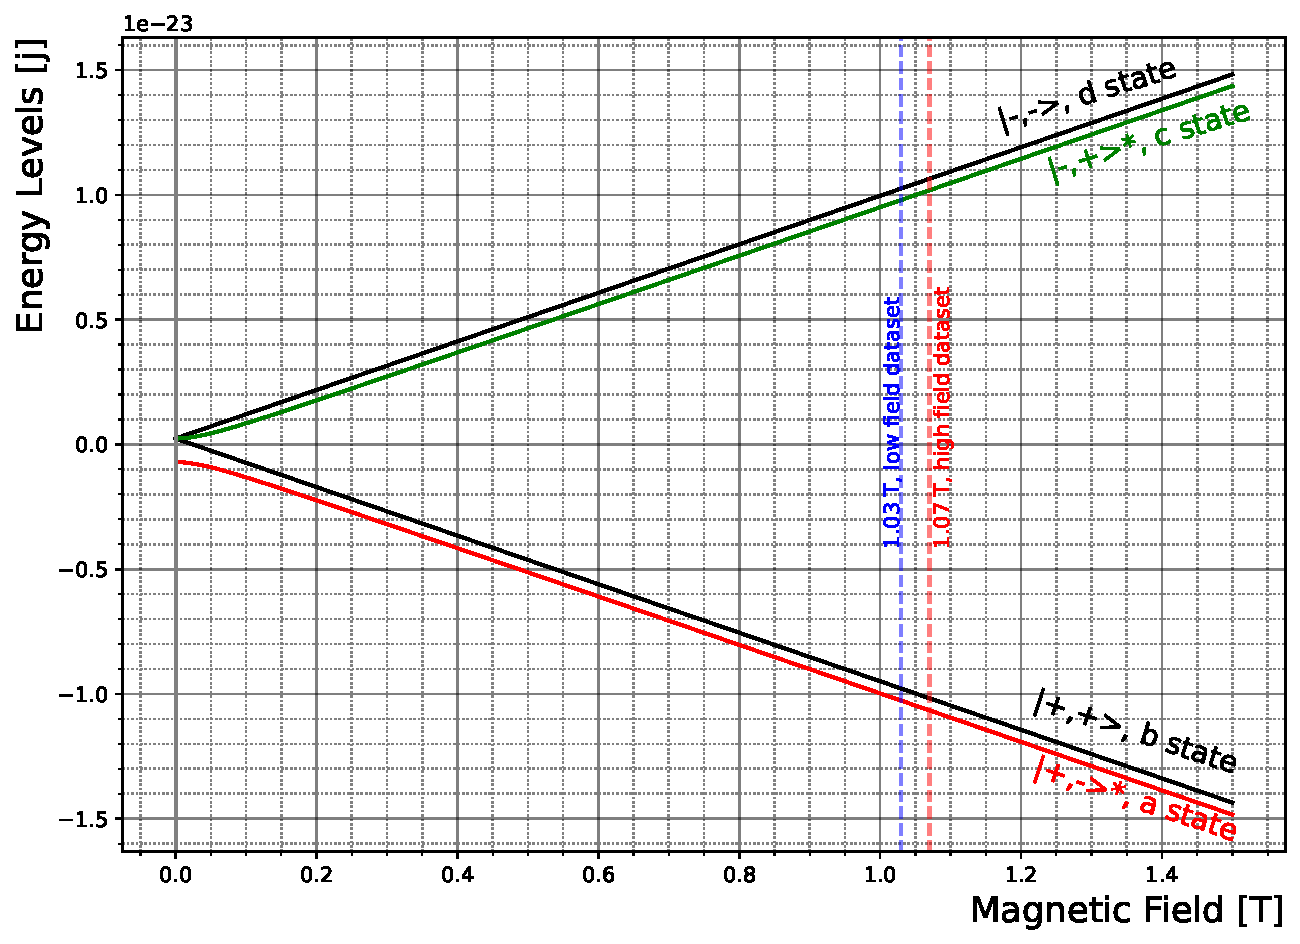
\includegraphics[width = \textwidth]{figures/chapter 3/HyperfineLevels.pdf}
\caption{Zeeman plot of the 4 hyperfine levels of the 1S state. The blue and red dotted lines denote the magnetic field configuration corresponding to the two datasets used for the measurement. Each of the four lines is labeled according to its spin configuration at high magnetic field regime. The \textbf{d} and \textbf{b} states correspond exactly to the parallel and antiparallel spin alignments (up-up and down-down) for the antiproton and positron. The \textbf{c} state and \textbf{a} state are mixed due to the presence of the external magnetic field, and only in the high field limit the states correspond to the up-down or down-up spin configuration.}\label{fig:ZeemanDiagram}
\end{figure}

As explained in Sec.~\ref{sec:antihydrogensynthesis}, the only trappable states are the \textbf{c} and \textbf{d}, which are the ``low-field seeking'' states. In high field regime, that is the case of the \ALPHA experiment (magnetic field at $\simeq$ \SI{1}{\tesla}), the hyperfine splitting is defined as the frequency difference between the transition from the \textbf{d} state to the \textbf{a} state and the transition from the \textbf{c} state to the \textbf{b} state.

\begin{equation}
f_{da} - f_{cb}  = \left[(E_d - E_a) - (E_c - E_b)\right] \frac{1}{2 \pi \hbar} = \dfrac{a_{1S}}{h}
\label{eq:hfsdiff}
\end{equation}

It is important to highlight that this relation is valid only if the two transitions are measured at the same magnetic field value. This point is particularly significant, as it introduces one of the key characteristics of the magnetic field in the experiment. In fact, the large superconducting solenoid in \ALPHA, the \textit{Carlsberg} magnet, produces a magnetic field that is affected by drift over time. The characterization of this drift is made through the ECR technique, which has been already discussed in Sec.~\ref{sec:ECRtecnique}. The ECR technique was used during the data taking as a complementary method to monitor the magnetic field variation over time. The ECR was performed at a specific location, which is \SI{261.8}{\milli \meter} \commento{explain why at this location}. The measurements are reported in Fig.~\ref{fig:ECR_term_bdrift}, that shows the magnetic field value measured at different times during the experiment. While the experimental protocol will be discussed later, it is evident from the Fig. that there is an initial transient phase, during which the magnetic field remains constant or exhibits an upward drift (attributed to fine scale flux relaxation following the solenoid reset). This is followed by a slower, long-term, downward linear drift of the field, due to the decay of persistent currents in the external solenoid. The linear drift of the magnetic field is expected to be negative, causing a shift in the resonance of the transitions of about \SI{70}{\kilo \hertz \per \hour}.

\begin{figure}[hbtp]
\centering
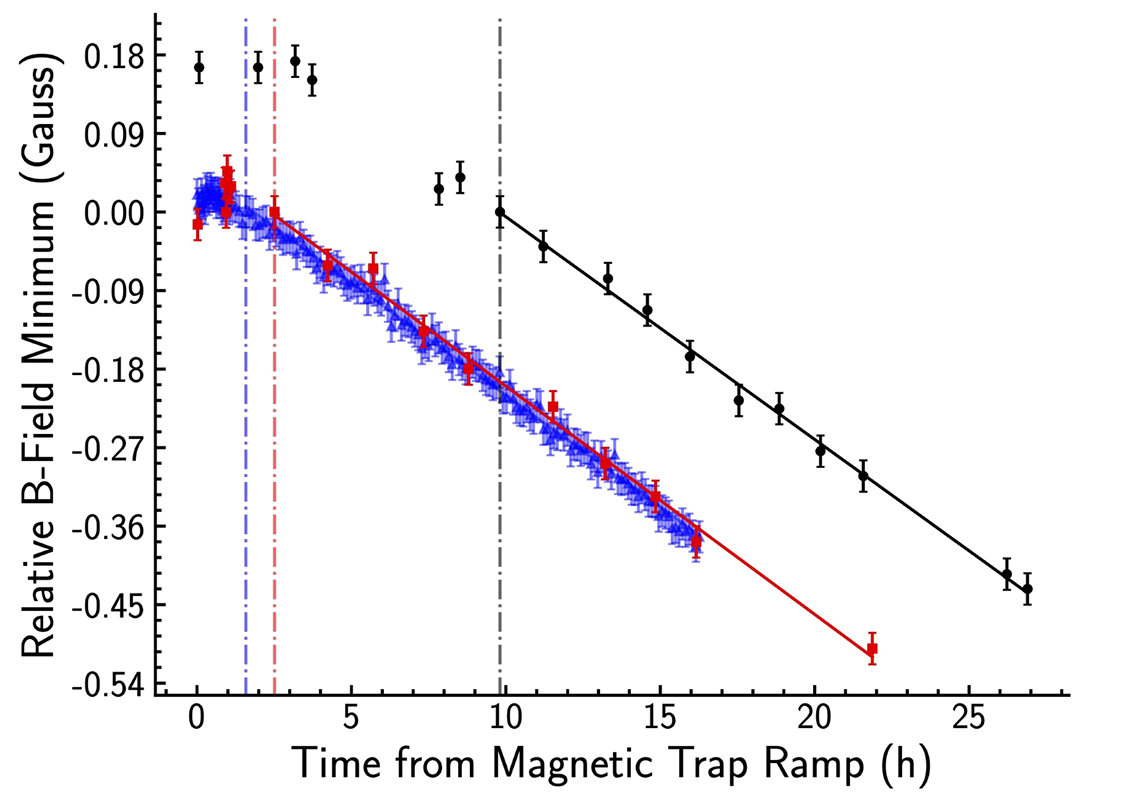
\includegraphics[width=\textwidth]{figures/chapter 3/ECR_plot_nature.png}
\caption{ECR measurement of the magnetic field drift over time. The two series of points show the trend of the magnetic field over time from the most recent reset of the \textit{Carlsberg} superconducting solenoid. The two datasets used for the measurement differ for a small offset of the magnetic field at the trap center ($\simeq$ \SI{0.04}{\tesla}).}
\label{fig:ECR_term_bdrift}
\end{figure}

\section{Experimental protocol} \label{sec:Protocol}
\contentof{Description of the experimental protocol: stacking, measurement scan from lower to higher frequencies ecc. Things to mention are: 
\begin{itemize}
\item destructive measurement: depletion effects
\item it's a measurement by difference! It's important to mention it!
\item Magnetic field profile
\item step duration, clearing...
\item qualitative interpretation of the shape: depletion effect, resonant volume ecc...
\end{itemize}
}

This section provides a detailed description of the experimental protocol followed during data collection. The experimental data for spectroscopy measurement at ALPHA are constituted by looking at the number of annihilating atoms over time. Depending on the different lines that the experiment aims to measure, various lasers, as the \SI{243}{\nano\meter} for the 1S--2S line, the \SI{121}{\nano \meter} for the Lyman-$\alpha$ or microwave light, are used to kick-out atoms, which annihilate on the trap walls. The physics processes involved can be different: for the 1S--2S spectroscopy, ionization and momentum transfer from the laser light to the atoms plays the main role, while for the hyperfine measurement, the positron spin flip from a trappable to un-trappable state is the main physics mechanism for the ejection of atoms.

\subsection{Microwave induced annihilation}

To probe the \cb and \da transitions, microwave light is delivered into the trap environment via the wave guide depicted in Fig.~\ref{fig:TrapScheme}. The frequency of the light is tuned within the range of \SI{28}{\giga \hertz}-\SI{31}{\giga \hertz}, selected based on the corresponding operating point from the \SI{1}{\tesla} magnetic field. The number of atoms available for spectroscopy at the ALPHA experiment have increased from a few tens to several hundreds/thousands of atoms \cite{Akbari:2025mli}, that are stacked by repeating the mixing cycles for several hours. At first, these atoms are evenly split between the \textbf{c} and \textbf{d} states, while \textbf{b} and \textbf{a} states remain unpopulated, since atoms produced in these states rapidly ($\approx$ \SI{10}{\milli \second}) escape and annihilate on the trap wall upon creation.
The transitions are probed by injecting microwave light inside the trap cavity at varying frequencies, in increasing steps of \SI{5}{\kilo \hertz} and \SI{8}{\second} time duration. By varying the frequency, the microwave light can drive a positron spin-flip of an atom, modifying its quantum state. Once an atom ends up in an un-trappable state, it annihilates on the trap wall, and the annihilation products (typically pions) are then detected by the Silicon Vertex Detector (SVD) surrounding the trap electrodes. By properly tuning the frequency of the microwave light, it is possible to select the \cb or the \da transition, and record different spectra from which physical quantities can be inferred.
The protocol used during the 2024 data taking comprises a number of 48 frequency steps, (for a total of \SI{240}{\kilo \hertz}), followed by a high power phase, named ``clearing'', consisting of 16 frequency steps of the same duration, during which residual \textbf{c}-state or \textbf{d}-state atoms that did not undergo a transition are removed. 
%Strictly speaking, the duration of the spectroscopy measurement was \SI{512}{\second}, during which several hundreds/thousands of atoms are recorded.

\subsection{Protocol of the spectroscopy experiment} \label{Protocol-of-experiment}
To measure the \fcb and \fda transition frequency, approximately 1400-1600 atoms are synthesized and trapped from repeating positron/antiproton mixing cycles over a period of $\approx$ \SI{1}{\hour}. During each mixing cycle, a total of 90/100 atoms are trapped in the \SI{0.5}{\kelvin} magnetic potential well. The microwave light is injected in the trap, first tuned to probe a single \cb transition, followed by a \da. To excite the \da transition, the microwave frequency scan starts at \SI{+1420390}{\kilo \hertz} above the starting frequency of the previous \cb transition, that is changed from repetition to repetition to account for magnetic field drift. The \cb transition is always probed before the \da , performing the experiment in the reverse order does not guarantee, for instance, that \cstate atoms do not undergo a transition, because of the Zeeman broadening effect (details provided later).
A pause, lasting 300s, divides the two spectroscopy phases, during which the microwave system is switched off to cool down the electrodes of the trap, with the goal of avoiding a deterioration of the vacuum conditions inside the trap cavity. A \fcb and \fda measurement constitutes a single replica, which has been repeated consecutively 8 times. At the end of the 8 repetitions, a high-statistics repetition, with several thousands of atoms, has been measured, and used as a ``control'' sample for systematic studies. This procedure has been repeated twice, yielding two datasets that differ in the magnetic field setting used for the spectroscopy. One dataset was taken at \SI{1.03}{\tesla} and the other at \SI{1.07}{\tesla}. We will refer to these as low-field and high-field datasets, respectively. These settings correspond to different on-axis field minima, achieved by adjusting the target current in the Carlsberg solenoid.

The purpose of the second dataset is not to test the field dependence of the splitting itself: as shown in Eq.~\ref{eq:hfsdiff}, $f_{da}-f_{cb}$ does not depend on $B$, provided that both transitions sample the same field. What changes when the field minimum is moved from \SI{1.03}{\tesla} to \SI{1.07}{\tesla} is the frequency of the microwaves, which shifts by about \SI{1.2}{\giga\hertz} for both transitions (from $\approx$\SI{28.2}{\giga\hertz} to $\approx$\SI{29.4}{\giga\hertz} for \cb). The electrode stack acts as a waveguide for the microwaves, and the spatial structure of the field at the location of the atoms (the position of nodes and antinodes of the component transverse to the static field, and the relative weight of travelling and standing waves) depends on frequency in a way that is not well known \cite{ALPHA:2026lbu}. A second dataset at a different field therefore repeats the measurement with a different microwave field configuration, and the comparison between the two results tests the systematic uncertainties connected to the lineshape (Sec.~\ref{sec:Reproducibility}).

Depending on the size of the field change, a second dataset addresses different questions. A small change, as in this work, mainly modifies the microwave field structure, and is used as a check of the systematic uncertainties. A larger change would test the Zeeman dependence predicted by the Breit--Rabi formula, and an even larger one could constrain exotic field-dependent couplings; neither is attempted here, since the second dataset is used for the systematic study. At the opposite end, on the shortest time scale, the short-term field drift studied with the 2023 data (Sec.~\ref{sec:ShortDrift}) is related to the order in which the two transitions are driven.

 An additional difference is that a high-statistics measurement, performed before the 8 standard repetitions, was included only for the series at low magnetic field. The experimental procedure, schematically shown in Fig.~\ref{fig:RepetitionScheme} for a single repetition, can be summarized as follows:

\begin{itemize}
\item Reset of the Carlsberg magnet to the desired current
\item Stacking phase
\item ECR
\item low power \cb sweep to identify the frequency start
\item ECR
\item \cb scan (48 steps) and clearing (16 steps)
\item \SI{300}{\second} of wait to cool down electrodes
\item \da scan (48 steps) and clearing (16 steps)
\item ECR
\end{itemize}

During the measurement, the ECR technique has been employed in between physical runs to monitor the magnetic field.


\begin{figure}[hbtp]
\centering
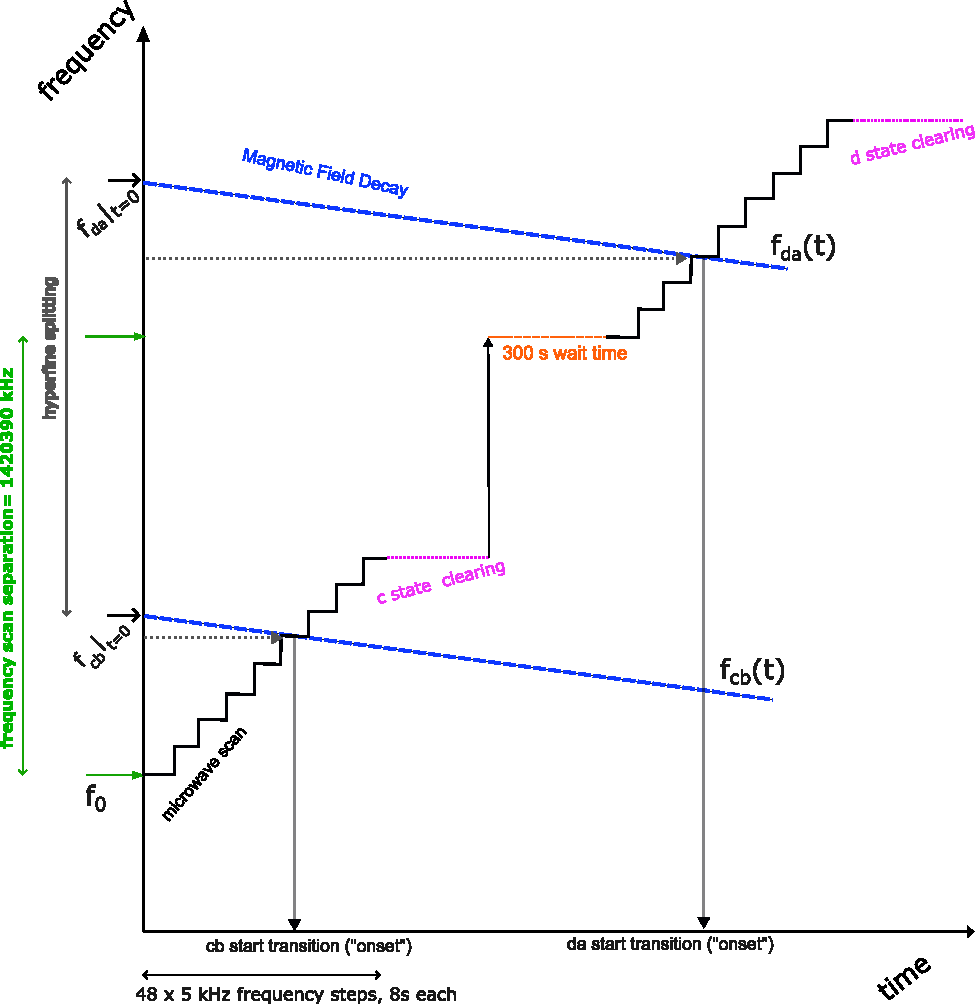
\includegraphics[width=\textwidth]{figures/chapter 3/SchemeBdrift.pdf}
\caption{Scheme of a single experimental repetition. Each dataset consists of 8 such repetitions, with atoms stacked between each run for the next cycle. The initial frequency $f_{0}$ of the first microwave sweep of the \fcb scan, is determined by a low power scan to locate the ``onset'' of the transition. For subsequent repetitions, the starting frequency of each sweep is adjusted by subtracting the expected magnetic field drift.}
\label{fig:RepetitionScheme}
\end{figure}

It is important to clarify that, in this context, the experimental spectra refer to the annihilation counts recorded by the SVD over time. These spectra are influenced by the depletion of the total atomic population available during the microwave sweep, and are shaped by several other factors, as the temperature of the atom sample, the unknown standing wave pattern, Doppler broadening, magnetic field inhomogeneities and the natural linewidth of the transition. The interplay of all these effects collectively determines the observed spectral shape. However, since the relevant physical quantity is obtained from the difference between \fcb and \fda transitions, the key point is the relative impact of these effects on the two transitions. In this sense, the ``by difference'' nature of the measurement is advantageous: systematic effects that affect both transitions similarly can partially, or even fully, cancel out.


\subsection{Magnetic field profile} \label{sec:MagFieldProfile}

\commento{Qui sei stato un po' sintetico. Sicuramente c'è da recuperare materiale aumentare questa parte}
Special attention was devoted to the design of the magnetic field. The magnetic field was shaped to reduce the second order-derivative. Physically, in presence of a ``steep'' magnetic field, the atoms traverse the field minimum rapidly, thereby reducing their interaction time with the microwave field necessary to induce transitions. Instead, for a flattened field profile, the region where the ``resonant'' frequency closely matches the injected microwave frequency is broader, which enhances the probability of transition. Fig.~\ref{fig:flatfield} shows the magnetic field profile in the vicinity of the global magnetic field minimum. The magnetic field is deliberately depressed below the central mirror coil (by a \SI{50}{\micro \tesla}) to create a well-defined absolute minimum. Neglecting all other effects that contribute to broadening, this results in a narrow and well-defined resonance frequency. During the frequency scan, the microwave frequency probes transitions associated with higher values of the magnetic field, and the spectra are therefore subject to Zeeman broadening.

\begin{figure}[hbtp]
\centering
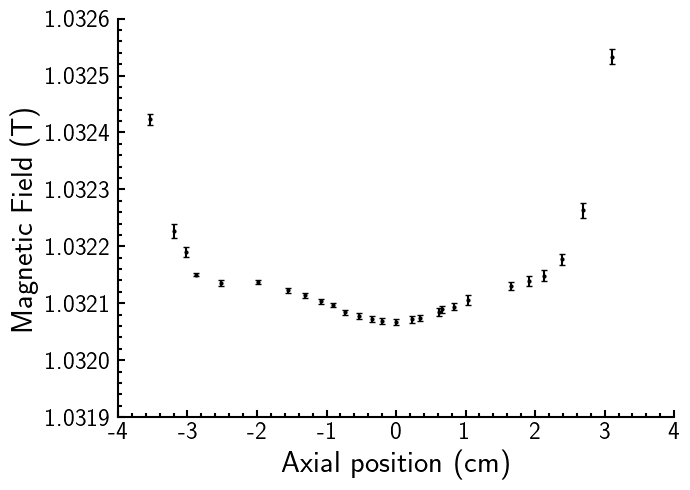
\includegraphics[width=0.75\textwidth]{figures/chapter 3/2024_MFF_DriftCorrected.png}
\caption{On-Axis magnetic field profile measured through ECR repeated at different Z position of the plasma. The spatial resolution of the technique is \SI{1}{\milli \meter}. The error bars on the $y$ axis represent the standard deviation of a Gaussian fit to the ECR signal.}
\label{fig:flatfield}
\end{figure}

The Zeeman effect also defines the order of the measurement: in principle one could measure the \fda transition first and the \fcb as the second. But by doing so, some of the c-state atoms could also contribute to the \fda signal, since they can explore a magnetic potential region that matches the resonance condition. While for the other order, the d-state atoms would need to explore a magnetic potential region below the actual field minimum. 
 

\subsection{Microwave system: power and duration} \label{sec:MWpower}
\contentof{Talk about the setup of the microwave system, issues with the energy distribution and not very well defined resonance, introduce the microvawe flat field for}

The microwave power is produced by an analog signal generator (Agilent 8257D PSG) and subsequently amplified by a Miteq AMF-4B amplifier. The microwaves are delivered into the trap volume through a vacuum window and waveguides. Prior to the experiment, the injected power is adjusted to produce similar transition lineshapes with a high-statistics sample, and matching the profiles of the \cb and \da transitions.
Variation in power delivered to the trap, as well as differences in the standing wave pattern can account for discrepancies in the shape between the two transitions, and therefore introduce a systematic error in the hyperfine measurement. The actual power in the trap and the standing wave pattern are not precisely known, and are expected to vary depending on the frequency of the injected microwave light. Therefore, part of the data analysis is devoted to estimating the systematic uncertainty associated with these variations. This will be discussed in detail in Chapter~\ref{ch:analysis}.
To choose the microwave power for the experiment, a series of lineshapes were measured while varying the microwave amplifier output power. The goal of this campaign was to balance the observed lineshapes and identify the power setting that yields the closest match between the \fcb and \fda transition profiles. The microwave intensity was changed by tuning the amplification of the microwave amplifier, which allows choosing from a range of several decibels of amplification. Some of the spectra collected at the high field are reported in Fig.~\ref{fig:PowerStudies}

\begin{figure}[htbp]
\includegraphics[width = \textwidth]{figures/chapter 3/Power_studies.pdf}
\caption{Lineshape collected with different nominal power of the microwave amplifier, for the set of data taken at \SI{1.07}{\tesla}, the frequency step is \SI{5}{\kilo \hertz}, with a pulse length of \SI{8}{\second}, \commento{spiegare cosa sono 12db}.}
\label{fig:PowerStudies}
\end{figure}
 
Regarding the step duration, that for the nominal datasets is \SI{8}{\second}, this has been selected by performing measurements with high-statistics runs, varying the time duration of microwave irradiation step, in the range of [\SI{1}{\second}, \SI{32}{\second}].

\begin{figure}[htbp]
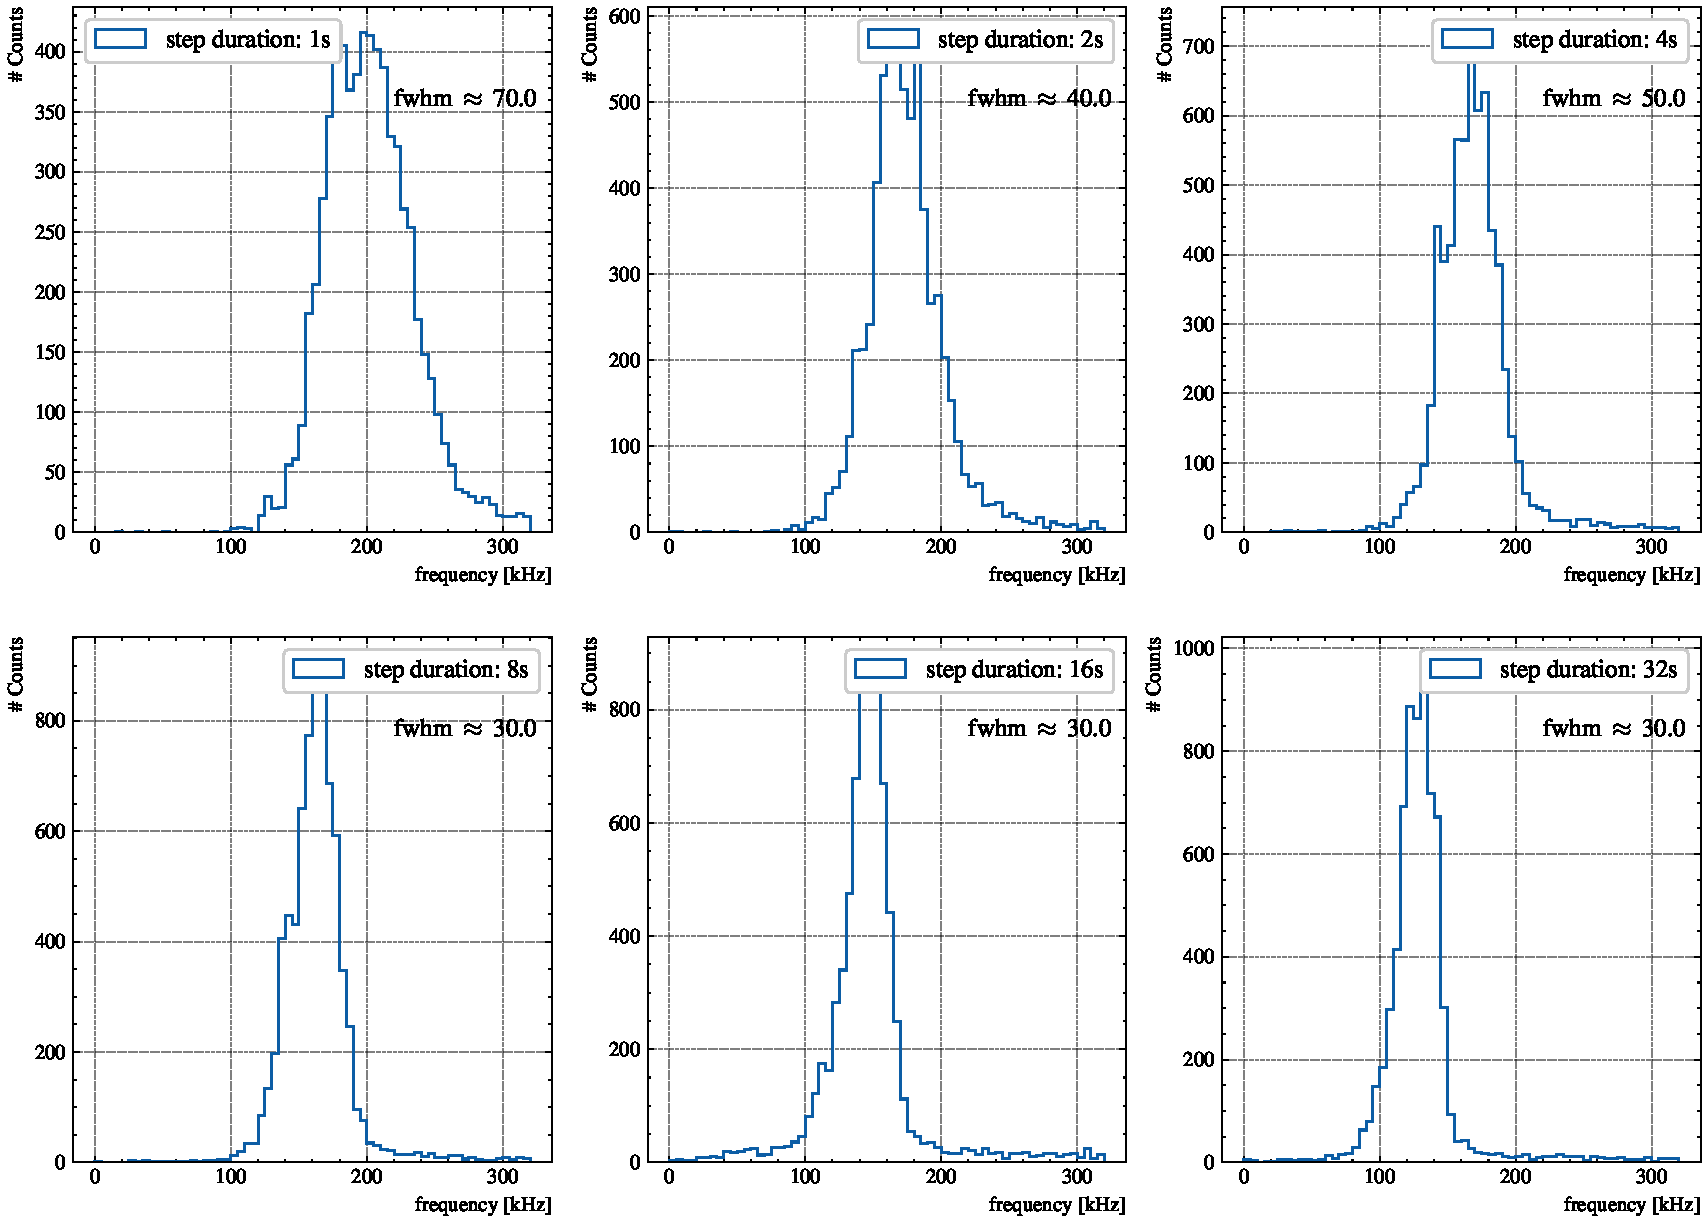
\includegraphics[width=\textwidth]{figures/chapter 3/Pulse_Length_studies.pdf}
\caption{Collection of high-statistics \fcb lineshapes measured for various pulse-length durations. The starting frequency is expressed arbitrarily as \SI{0}{\kilo \hertz}.}
\label{fig:PulseLengthStudies}
\end{figure}

The distributions in Fig.~\ref{fig:PulseLengthStudies} have been interpreted as follows: when the microwave frequency approaches the value corresponding to the magnetic field minimum, atoms begin to be ejected from the trap and subsequently annihilated. The probability of ejection is proportional to the duration for which the atoms remain in the vicinity of their resonance condition while exposed to the microwave field. For shorter microwave pulse duration, some atoms capable of undergoing transitions at a given frequency may not be ejected due to insufficient pulse length. This accounts for a broader full width at half maximum (FWHM) observed for the \SI{1}{\second} case. Increasing the pulse duration leads to a decrease in FWHM, and from \SI{8}{\second} to \SI{32}{\second} the spectra converge to a FWHM of \SI{30}{\kilo\hertz}. The behavior indicates that for duration longer than \SI{8}{\second}, the pulse is sufficiently long for all atoms at each microwave step that are able to undergo a transition to do so, resulting in a ``saturation'' of the spectra lineshape.
Following this interpretation, the step duration has been fixed to \SI{8}{\second}. Longer pulses do not offer any benefit in terms of the width of the lineshape; on the other hand, they contribute more to heating the trap electrodes, resulting in a worse vacuum condition and potentially more background due to annihilation of residual gas inside the trap.


\section{Qualitative interpretation of the observed spectra}

In the previous section some \fcb and \fda spectra have been presented. As anticipated before, the measured lineshapes are the convolution of several physical phenomena that broaden the natural linewidth of each transition. A qualitative interpretation of the experimental lineshape can be offered by looking at the magnetic field profile in Fig.~\ref{fig:flatfield}. As the microwave frequency gets closer to the corresponding value at the minimum magnetic field, the small percentage of the trapped atoms begins to annihilate (transition onset). At the beginning, only the atoms which pass through the magnetic field minimum are sensitive and can effectively undergo a transition. While the microwave scan proceeds toward higher frequency, the ``resonant volume'' increases, and so more atoms whose trajectory is not crossing the magnetic field minimum, are kicked out. Since the total number of atoms is fixed at the beginning of the experiment, the right part of the spectrum is dominated by depletion effects. The lineshape can be approximately divided into three sections: a rising left tail, corresponding to probing in the proximity of the magnetic field minimum, a central part which describes the increase of the resonant volume as the scan proceeds, and a decreasing right tail, due to depletion effects.



\chapter{Data Analysis And Systematic Uncertainties}
\label{ch:analysis}

This chapter describes the statistical and mathematical framework used to analyze the data collected during the 2024 antihydrogen ground-state hyperfine splitting campaign. The improvements in trapping efficiency, magnetic field design, colder energy distribution and characterization of the magnetic field drift, together with new analysis techniques, have all contributed to an improvement of \num{e2} compared to the first observation made by the ALPHA collaboration in 2017 \cite{ALPHA:2017fsh}.

The 2024 dataset consists of two complete spectroscopy campaigns performed at different magnetic-field configurations, together with dedicated auxiliary measurements, including electron cyclotron resonance (ECR) magnetometry and high-statistics calibration samples. These auxiliary datasets play a crucial role in the characterization of the magnetic-field evolution and in the evaluation of systematic uncertainties.

The analysis follows a frequentist approach and is implemented within the \textit{ROOT} and \textit{RooFit} frameworks using a Python-based \textit{PyROOT} analysis package. The model parameters are determined through a maximum-likelihood fit, with numerical minimization performed using the \textit{MINUIT2} optimizer.

The first stage of the analysis consists of a simultaneous fit to the frequency distributions associated with the \cb and \da positron spin-flip transitions. An empirical line-shape model is fitted to all repetitions within a given experimental series. While several parameters describing the overall line shape are shared among the repetitions, specific parameters are allowed to differ between the two transitions in order to account for residual differences in their spin-flip dynamics. The outcome of this fit is a set of frequency markers that characterize the onset of each transition.

These frequency markers should not be interpreted as direct measurements of the absolute resonance frequencies. Owing to the presence of several broadening mechanisms, including magnetic-field inhomogeneities, motional effects, and finite interaction times, the observed spectra do not provide a direct determination of the resonance position. Instead, the analysis is designed as a differential measurement, focusing on the precise extraction of reproducible frequency markers whose difference can be related to the physical hyperfine splitting.

In a second step, the extracted frequency markers are corrected for the time-dependent drift of the magnetic field following the most recent reset of the Carlsberg solenoid. For each dataset, the markers obtained from the eight repetitions of the two transitions are combined in a common linear fit that accounts for the correlated magnetic-field evolution. The separation between the two fitted lines provides an estimate of the ground-state hyperfine splitting, while correlations and systematic effects are propagated to the final result.

\section{Background Model}

In the analysis, a flat distribution for the background is considered. The main source of background is constituted by cosmic events, mainly muons, that are wrongly recorded as annihilations from the Silicon Vertex Detector. The cosmic background has been decreased by employing multi-variable-analysis techniques that employ information on the event topology (Fig.~\ref{fig:MVAscan}).

\begin{figure}[!hbtp]
\centering
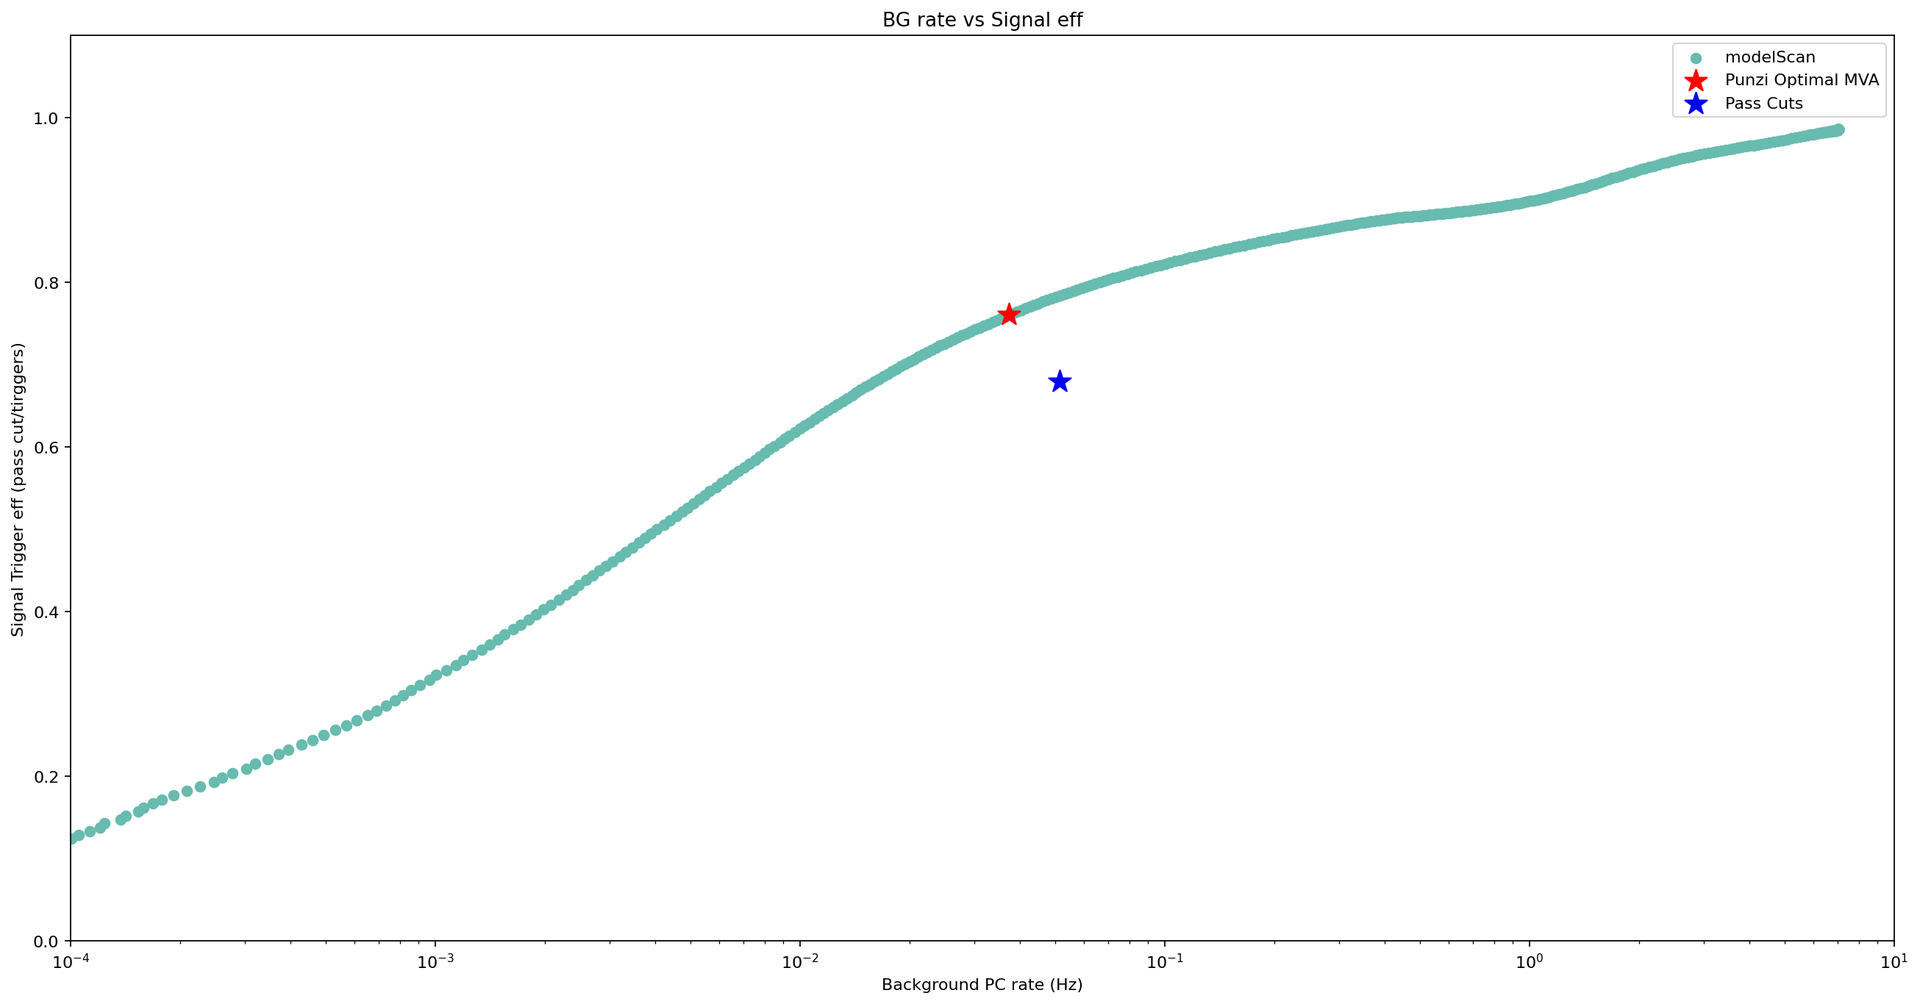
\includegraphics[width = \textwidth]{figures/chapter 4/MVA-punzi.png}
\caption{MVA scan plot. The cyan curve represents scan of the MVA model varying the selection criteria. The red star is the optimal point corresponding to the minimization of the Punzi figure of merit \cite{punzi2003sensitivitysearchesnewsignals}. The MVA curve is obtained by training the algorithm on data without \Hbar trapped, recording only annihilations from muons, and annihilations recorded during the mixing phase, during which the background is negligible and events are mainly constituted by un-trapped \Hbar .}
\label{fig:MVAscan}
\end{figure}

The cosmic background corresponding to the red star is the chosen working point, and the data that will be presented are related to that particular selection criterion. The signal efficiency rate is 75.7(5) \%, and the background is \SI{37.4(7)}{ \milli \hertz}. 
Although these quoted values are estimated from runs with several thousand recorded events, the actual background during the experimental runs can be different. Due to the presence of electrode heating, a portion of the atoms could annihilate on residual gas. The amount of gas present in the trap is not controlled, hence the background is a free parameter in the analysis, and has not been fixed to the expected value from the MVA selection.

\section{Signal Model Definition}

%In the analysis model, it is used for the {\it frequency marker} a definition related to the onset of the transition. With respect to previous measurement \cite{ALPHA:2017fsh}, however, some modifications are necessary, to account for the increased $\overline{\mathrm{H}}$ population in each run (which may result in detectable background from anti-atoms escaping the trap for reasons different than microwave-induced spin-flips) and for the increased sensitivity to differences between the \cb and \da lineshapes. 

The lineshape model $f(\cdot)$ for the fit of the experimental data is constructed as the convolution of two functions: a bare function $g(\cdot)$ and a resolution/broadening function $R(\cdot)$:

\begin{equation}
\centering
f \equiv g \otimes R \,.
\label{eq:conv}
\end{equation}

The bare function $g$ is introduced to describe the energy distribution, magnetic field profile, and depletion effects which determine the lineshape. It has a well-defined onset of the transition, and an exponentially decaying right tail. The resolution function has been introduced to describe all those effects that are related to broadening of the resolution conditions, such as magnetic field inhomogeneities, magnetic field fluctuations, Doppler broadening, and transit-time broadening.
The function has been expressed in terms of a parameter that describes the frequency position of the \cb and \da lineshapes, and acts therefore as a \textit{frequency marker} ($f_o$). Although tempting, these frequency markers are only related to the resonance frequency at a given condition, because of several broadening effects that will be discussed later in this chapter. The difference of the frequency markers for the \cb and \da transitions, corrected for the magnetic field decay, is an estimate of the antihydrogen hyperfine splitting frequency $a_{1S}/h = f_o^{(da)} - f_o^{(cb)}$. 
The actual shape of $g$ cannot be derived directly from first principles, since it would require knowledge of the microwave standing wave pattern, the actual power delivered to the trap, and the energy distribution of the atoms. These quantities are not known with enough precision, hence the signal model corresponds to an empirical function which satisfies the following requirements:

\begin{itemize}
    \item its value is zero for frequency values lower than $f_o$, and strictly positive for frequencies higher than  $f_o$; 
    \item it features a monotonic rise (corresponding to an increase in the resonant volume as the frequency is increased) between $f_o$ and the maximum of the function;
    \item it features a monotonic decay (associated to the decreasing antihydrogen population as the scan progresses) after the maximum.
\end{itemize}

The bare function $g$ is described by Eq.~\ref{eq:model1}:

\begin{equation}
\centering
g(\overline{x})=
\begin{dcases}
 0        & \overline{x} < - \sigma (k + 1) \\
\exp\left(-\frac{1}{2}\right) \times \left[\frac{\overline{x} + \sigma (k + 1)}{\sigma k}\right]^k  & [\overline{x} > - \sigma (k + 1)] \land (\overline{x}<- \sigma) \\
\exp\left(-\frac{\overline{x}^2}{2\sigma^2}\right)  & (\overline{x} >-\sigma) \land (\overline{x}<0) \\
\exp\left(-\frac{\overline{x}^2}{2\sigma_r^2}\right) & (\overline{x} >0) \land (\overline{x}< \sigma_r) \\
\exp\left(-\frac{1}{2}\right)\left[\frac{\overline{x} + \sigma_r(n-1) } {\sigma_rn} \right]^{-n} & \overline{x} > \sigma_r \\
\end{dcases}
\label{eq:model1}
\end{equation}

The onset (our chosen frequency marker) is defined as the minimum value at which the above equation differs from zero, while the function parameters have the following meaning:

\begin{itemize}
    \item $\overline{x} \equiv x - x_{max}$. Therefore, $\overline{x} = 0$ is the position of the maximum;
    \item $\sigma$ is the standard deviation for the left-side Gaussian-like component;
    %    \item $-b\sigma$ represents the connection point between the polynomial rise and the Gaussian;
    \item $k$ is the degree of the polynomial describing the rise portion; 
    %\item $r = \sigma \cdot \frac{k + b^2}{b}$ 
    %    \item $C= \exp(-\frac{b^2}{2})$ ensures the continuity in the function;
    \item $r = \sigma \cdot (k + 1)$ is the distance (rise length) between the onset and the maximum;
    %\item $a$ describes the weight of the right-side non-Gaussian tail;
    \item $\sigma_{r}$ is the  standard deviation of the right-side Gaussian core portion, while $n$ describes the power-law right-tail (Crystal Ball function).  
\end{itemize}

Although complex, the core of this model has been developed considering a power law rise to describe the early part of the lineshape, and an asymmetric tail to describe the later part of the lineshape, and imposing continuity and first-order differentiability at the junction point.
To gain some physical intuition on the model, one can think of the bare function $g$ as describing the lineshape we would observe if the atoms were stationary, the microwave radiation monochromatic, the magnetic field perfectly stable, etc., i.e., if all broadening sources were turned off. 

In this hypothetical case, for an upward microwave frequency ramp, the onset would be well defined: it would correspond to the infinitely-large sample-size limit of the minimum value corresponding to the first significant annihilation count, and would be associated with the lowest value of the magnetic field. In practice, since the experiment is not dealing with stationary atoms and a perfect magnetic field, a certain level of broadening is expected.

\subsubsection{The resolution/broadening function} \label{sec:resolutionF}

Simulations show that spin-flip transitions can occur at frequencies lower than the frequency corresponding to the magnetic field minimum, due to effects such as: 
\begin{itemize}
    \item \textbf{Fluctuations in the magnetic field.} The resonance condition is set by the magnetic field at the trap minimum, and near \SI{1}{\tesla} the positron spin-flip frequencies change by about \SI{28}{\giga\hertz} per tesla \cite{ALPHA:2026lbu}. A field change as small as \SI{0.4}{\micro\tesla}, less than one part per million of the bias field, therefore moves the resonance by about \SI{10}{\kilo\hertz}. The currents in the trap magnets are actively stabilized to within a few mA, but small residual fluctuations and short glitches remain (Sec.~\ref{sec:DCCTs}): whenever the field at the minimum is momentarily lower, atoms can come into resonance at a microwave frequency below the nominal onset.
    \item \textbf{Width of the microwave radiation in the trap.} The radiation is produced by a synthesizer referenced to a \SI{10}{\mega\hertz} signal provided by CERN, so the intrinsic spectral width of the injected radiation is negligible compared with the \SI{5}{\kilo\hertz} frequency step \cite{ALPHA:2026lbu}; annihilations occurring while the synthesizer settles to a new frequency ( $\approx$ \SI{30}{\milli\second} after each step) are vetoed. More relevant is the fact that the radiation reaches the atoms through the electrode stack as a superposition of standing and travelling waves, whose amplitude and polarization change with position. An atom therefore experiences a microwave field whose strength varies along its trajectory, which mainly affects the transition rate, as discussed below for power broadening.
    \item \textbf{Doppler-shift broadening.} An atom moving along the propagation direction of the radiation sees the microwave frequency shifted by a fraction $v_z/c$. For the energies of the trapped atoms (below \SI{0.5}{\kelvin}) this shift is a few kHz, as estimated in Sec.~\ref{sec:Doppler}. Since the frequency is scanned from below, only the atoms that see the radiation shifted upwards matter, as they come into resonance before the nominal onset; the resulting contribution is therefore one-sided.
    \item \textbf{Transit-time broadening.} An atom does not sit at the field minimum, but moves through the trap, and stays in resonance only for the short time it takes to cross the region where its detuning is small. A transition driven for a finite time $\tau$ is not sharp in frequency, but has a width of order $1/\tau$: for example, an effective interaction time of \SI{0.1}{\milli\second} corresponds to a width of about \SI{10}{\kilo\hertz}. Atoms crossing the minimum can therefore undergo a spin flip even if the microwave frequency is slightly below the resonance frequency at the minimum.
    \item \textbf{Power broadening.} A stronger microwave field drives the spin flip faster, and the range of detunings over which a transition can still occur becomes wider, roughly in proportion to the amplitude of the oscillating magnetic field (the Rabi frequency). This effect is visible in the simulations, where the fitted broadening increases with the microwave field amplitude (Tab.~\ref{tab:resfun}). Since the power that reaches the atoms depends on frequency, it can differ between the two transitions: this is why the injected powers are balanced (Sec.~\ref{sec:MWpower}), and why the residual difference is included in the systematic uncertainty.
\end{itemize}

Transit-time and power broadening are included in the simulations, which compute the spin-flip probability along each trajectory with a time-dependent detuning \cite{ALPHA:2026lbu}, while the Doppler effect is not, and is estimated separately (Sec.~\ref{sec:Doppler}).

Estimating the size of these effects from simulations or calculations is expected to be an easier task than simulating the full lineshape, at least under a set of reasonable simplifying assumptions. Therefore, we describe such broadening effects in the model by convolving the bare function $g$ with the resolution function $R$. The parameters of the resolution function are determined from simulations and calculations, and are fixed in the fit to the \Hbar data, i.e., there are no floating parameters associated with the resolution function in the fit to the data.

Since monotonic upward frequency scans are performed in the experimental runs, the broadening function is one-sided. This choice assumes that a negligible portion of the atoms whose frequency matches the microwave frequency during the scan will evade transition. This could apparently conflict with the fact that a certain amount of atoms do not undergo a transition, and are finally ejected during the \textit{clearing} scan. However, there are physical mechanisms that can explain this: in fact, the evidence from the simulation indicates that the trajectories of antihydrogen atoms are chaotic. Hence, even though during the scan a certain resonant volume is depleted, it is not assured that some of the atoms won't repopulate a specific resonant volume further during the scan.

The approach followed in this analysis uses a resolution function whose shape and width can be varied to determine systematic uncertainties. The simulations were used to test different combinations of bare function $g$ and broadening function $R$.
The broadening function might depend on the step in the scan (i.e., might vary with frequency), but we can assume that the only part affecting the zero frequency marker is the one evaluated at the first significant step. 

The broadening may also depend on the population kicked out in the first step, which might in principle differ between the two transitions. % (i.e., there is a dependence on power); 

Even if the two broadening functions were the same, a different underlying bare function would result in a different effect on the {\it frequency marker}, which wouldn't cancel in the difference between the two transitions. 

We can assume different shapes for the broadening function, such as a one-sided Gaussian or a one-sided cusp. A right-sided tail (of negligible width, $t_R = 0.2\,{\rm kHz}$, compared to the frequency step) is included for numerical stability. For a Gaussian we have: 

\begin{equation}
\centering
R(\overline{x})=
\begin{dcases}
 \exp\left(-\frac{1}{2}\frac{x^2}{t_{gauss}^2}\right)        & x < 0 \\
 0 & x \geq 0\\
% \exp\left(-\left|\frac{x}{t_R}\right|\right)        & x \geq 0 \\
\end{dcases}
\label{GaussR}
\end{equation}
while for a one-sided cusp:
\begin{equation}
\centering
R(\overline{x})=
\begin{dcases}
 \frac{1}{t_{cusp}}\exp\left(-\frac{x}{t_{cusp}}\right)        & x < 0 \\
0        & x \geq 0 \\
\end{dcases}
\label{CuspR}
\end{equation}

An example of the bare function $g$ and of its convolution with the resolution function, fitted to the first repetition of a dataset, is shown in Fig.~\ref{fig:ModelVsData}.

\begin{figure}[!hbtp]
\centering
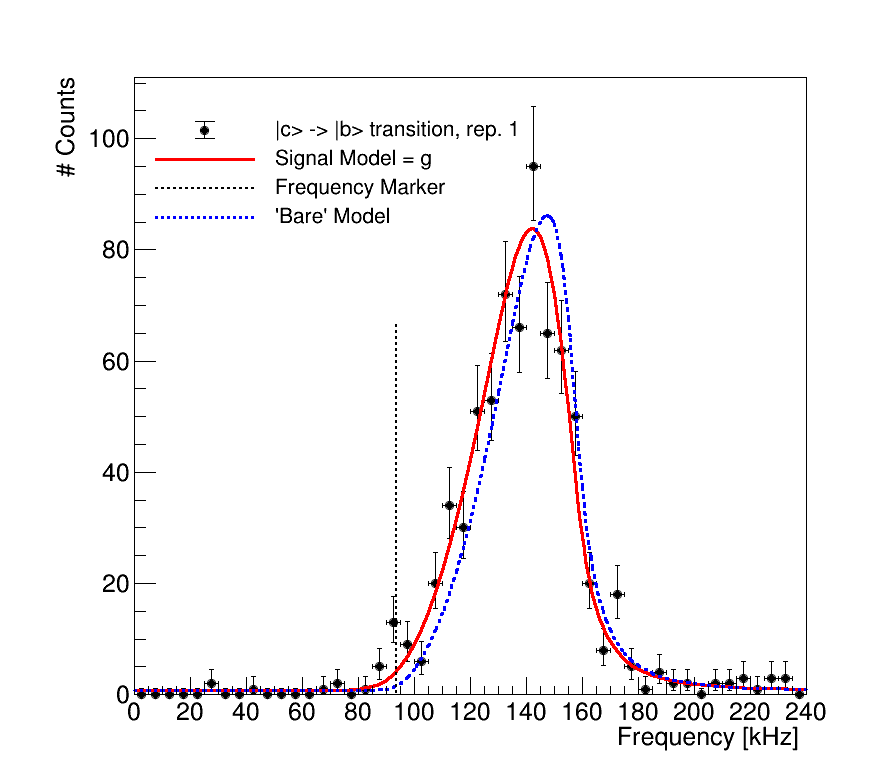
\includegraphics[width = \textwidth]{figures/chapter 4/Model_vs_data_s8.png}
\caption{Lineshape of the first repetition of the low field (\SI{1.03}{\tesla}) dataset. The blue line represents the bare function $g$ with best fit parameters. The red line represents the bare function $g$ convoluted with the resolution function (one-sided Gaussian with \SI{10}{\kilo\hertz} standard deviation), the black vertical dotted line is the frequency marker or onset position.}
\label{fig:ModelVsData}
\end{figure}

\section{Simulation} \label{sec:Simulation}

\contentof{In this section explain the simulation and how it has been used to estimate the systematic. The shown the plot of the simulation lineshapes and describe the limits of the simulation.}

Simulations of the experiment, involving antihydrogen motion and its interaction with microwaves, have been conducted to inform the model parameters and study some of the systematics of the measurement. The simulation reflects the experimental protocol, following the magnet manipulations and the frequency ramps. The magnetic field has been tuned using ECR data, the ones shown in Fig.~\ref{fig:flatfield}.

The simulation cannot describe the experiment with the required precision because of the lack of knowledge of the magnetic field off-axis and the unknown microwave field pattern in the trap. Therefore, the simulation has been used to inform the signal model parameters, such as the degree of the power-law rise of the lineshape. Different lineshapes corresponding to different microwave powers are available (Fig.~\ref{fig:SimLineshapes}), and have been fitted with the current signal model. Based on these fits (Tab.~\ref{tab:resfun}), the degree of the power-law rise has been fixed to $k=2$ in the nominal analysis, and the broadening parameters to $t^{cb}_{gauss} = t^{da}_{gauss} = \SI{10}{\kilo\hertz}$, half-way between the results obtained for the 2023 and 2024 simulations.

\begin{figure}[!hbtp]
\centering
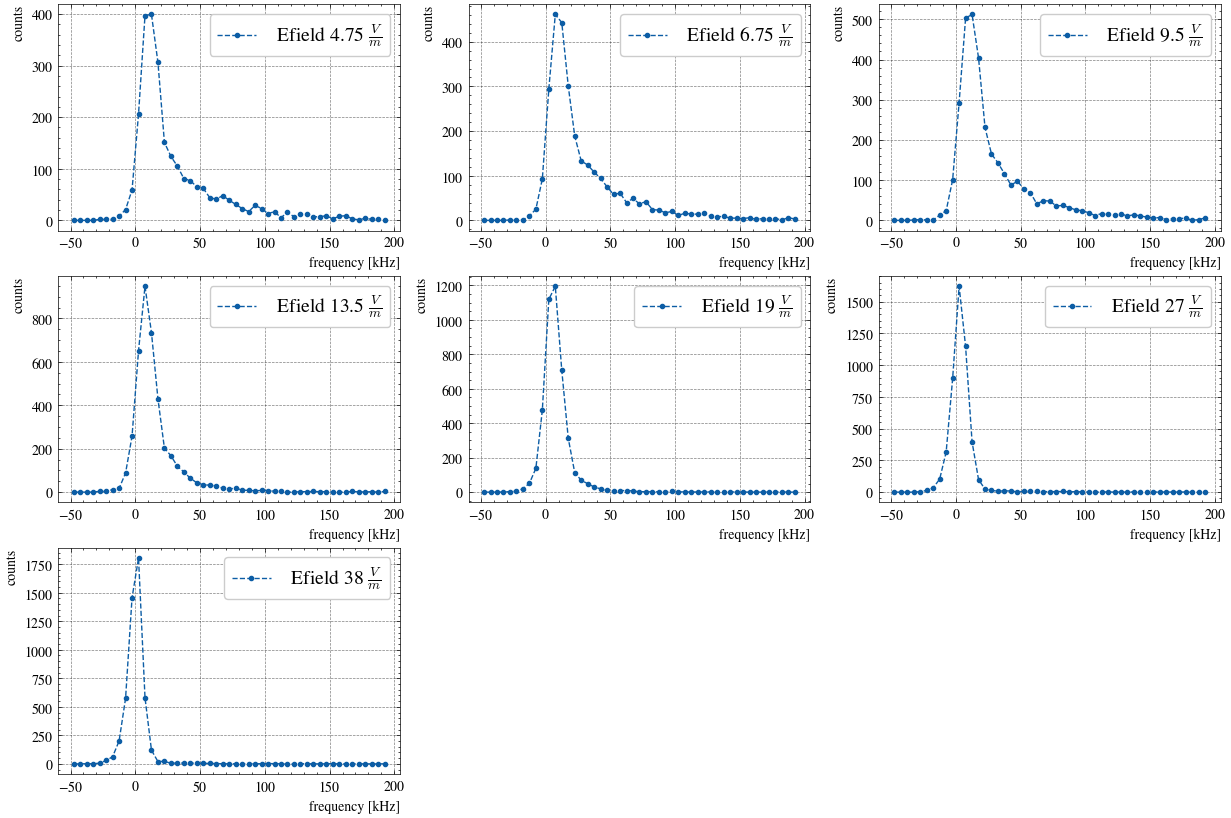
\includegraphics[width=\textwidth]{figures/chapter 4/FrancisSimulation_2024.png}
\caption{ Simulation of microwave induced annihilation for different electric field amplitudes (in legend reported as \SI{}{\volt\per\meter}). The simulation does not account for differences in the standing wave pattern for the \cb and \da transitions; consequently, the simulated \da lineshape is essentially identical to the \cb one, aside from the frequency offset corresponding to the splitting.}
\label{fig:SimLineshapes}
\end{figure}



\section{Maximum Likelihood Fit} \label{sec:MLEfit}

The analysis approach to extract the splitting from the raw data has been developed using the frequentist framework, where the best-fit parameters result from the maximization of the likelihood function \likelihood. As mentioned in Sec.~\ref{sec:Protocol}, the data are divided into two sets of eight repetitions, each consisting of a single \cb and \da transition measurement interspersed with stacking phases. Details of the specific runs and available data are reported in Tab.~\ref{tab:ListOfRuns}. 

\begin{table}[!ht]
    \centering
    \begin{tabular}{l|cccc}
         \hline\hline
% SERIES 7 ___________________
      {\bf \SI{1.07}{\tesla} dataset} & & & & \\
          {\bf Carlsberg reset}  & \multicolumn{3}{l}{19 May 2024: reset to 194.358 A} & 12:40     \\
    {\bf Repetition}   & {\bf Run}  & {\bf cb Init Freq (kHz)} & {\bf Unix Time (s)} & {\bf Time}  \\
          \hline

         
         0              &   70377   &$29\,418\,364$	 & 1716123393.873294	& 14:03 \\ 
         1              &   70378   &$29\,418\,284$	 & 1716129652.988256	&  \\ 
         2              &   70379   &$29\,418\,187$	 & 1716135002.727111	&  \\
         3              &   70380   &$29\,418\,073$	 & 1716140853.490512	&  \\ 
         4              &   70381   &$29\,417\,956$	 & 1716146112.077295	&  \\ 
         5              &   70382   &$29\,417\,741$	 & 1716155966.214942    &  \\ 
         6              &   70383   &$29\,417\,607$	 & 1716162057.169858    &  \\
         7              &   70384   &$29\,417\,488$  &  1716167889.394672	&  \\
         \hline
         (bkg study)    &   70385   &                &  	                &  \\
         post           &   70386   & $29\,416\,964$ & 1716193095.703465    & 10:48 (+1d) \\
         \hline
         \hline
% SERIES 8 ___________________
         {\bf \SI{1.03}{\tesla} dataset} & & & & \\
         {\bf Carlsberg reset} & \multicolumn{3}{l}{23 May 2024: reset to 186.426 A} & 13:13 \\
         {\bf Repetition}      & {\bf Run}  & {\bf cb Init Freq (kHz)} & {\bf Unix Time (s)} & {\bf Time} \\
          \hline 
         0            & 70462   & $28\,227\,463$	&	1716497309.208071	& 22:38 \\ 
         1            & 70463   & $28\,227\,387$	&	1716502378.209453	& \\ 
         2            & 70464   & $28\,227\,231$	&	1716509895.094319	& \\
         3            & 70465   & $28\,227\,132$    &	1716514501.176821	& \\ 
         4            & 70467   & $28\,226\,914$	&	1716524509.825337	& \\   
         5            & 70468   & $28\,226\,811$	&	1716529827.672246	& \\
         6            & 70469   & $28\,226\,710$	&	1716534513.851191	& \\
         7            & 70470   & $28\,226\,613$	&	1716539621.420382	& \\
         \hline
         pre          & 70461   & $28\,227\,609$	&	1716492680.251725	& 21:28       \\
         post         & 70471   & $28\,226\,227$    &	1716558788.451213	& 15:53 (+1d) \\
       \hline
       \hline
    \end{tabular}
    \caption{List of runs used in the analysis of the two datasets at lower and higher B-field. The initial frequency of the \da scan is set $1\,420\,390\,{\rm kHz}$ above the initial frequency of the \cb scan.}
    \label{tab:ListOfRuns}
\end{table}

The time interval between a run and the next one is \SI{1}{\hour} during which antihydrogen is accumulated in the trap by repeating mixing cycles of 4 minutes each. The total number of atoms accumulated for each run is $1400-1600$, equally split between the c and d states. The Maximum Likelihood fit consists in analysing the data simultaneously, with a likelihood defined as the sum of the individual likelihoods for each repetition:

\begin{equation}
\mathcal{L}_{tot} = \sum_{cb;da} \sum_{i} \mathcal{L}_{i}(\vec{\mu}, \vec{x})
\end{equation} 

Where $\vec{\mu}$ is the parameter space and $\vec{x}$ are the observations. The total likelihood is the sum of the likelihoods of each individual spectrum, and the minimization acts on the total likelihood. The advantage of this shared minimization is that the model complexity can be reduced, since some of the parameters are shared among repetitions of the same transition, increasing the statistical power for the fit of the shape parameters and improving the fit minimization. In the nominal analysis, the parameters controlling the shape of the spectra ($\sigma, \sigma_{r}, n_{r}$) are shared among repetitions of the same transition, while the normalization $nS_{i}$, the background, and the frequency markers $f_{cb,da;i}$ are individual for each repetition. As an example, the result of the fit for a single repetition is shown in Fig.~\ref{fig:ExampleSpectra}.

\begin{figure}[!hbtp]
\centering
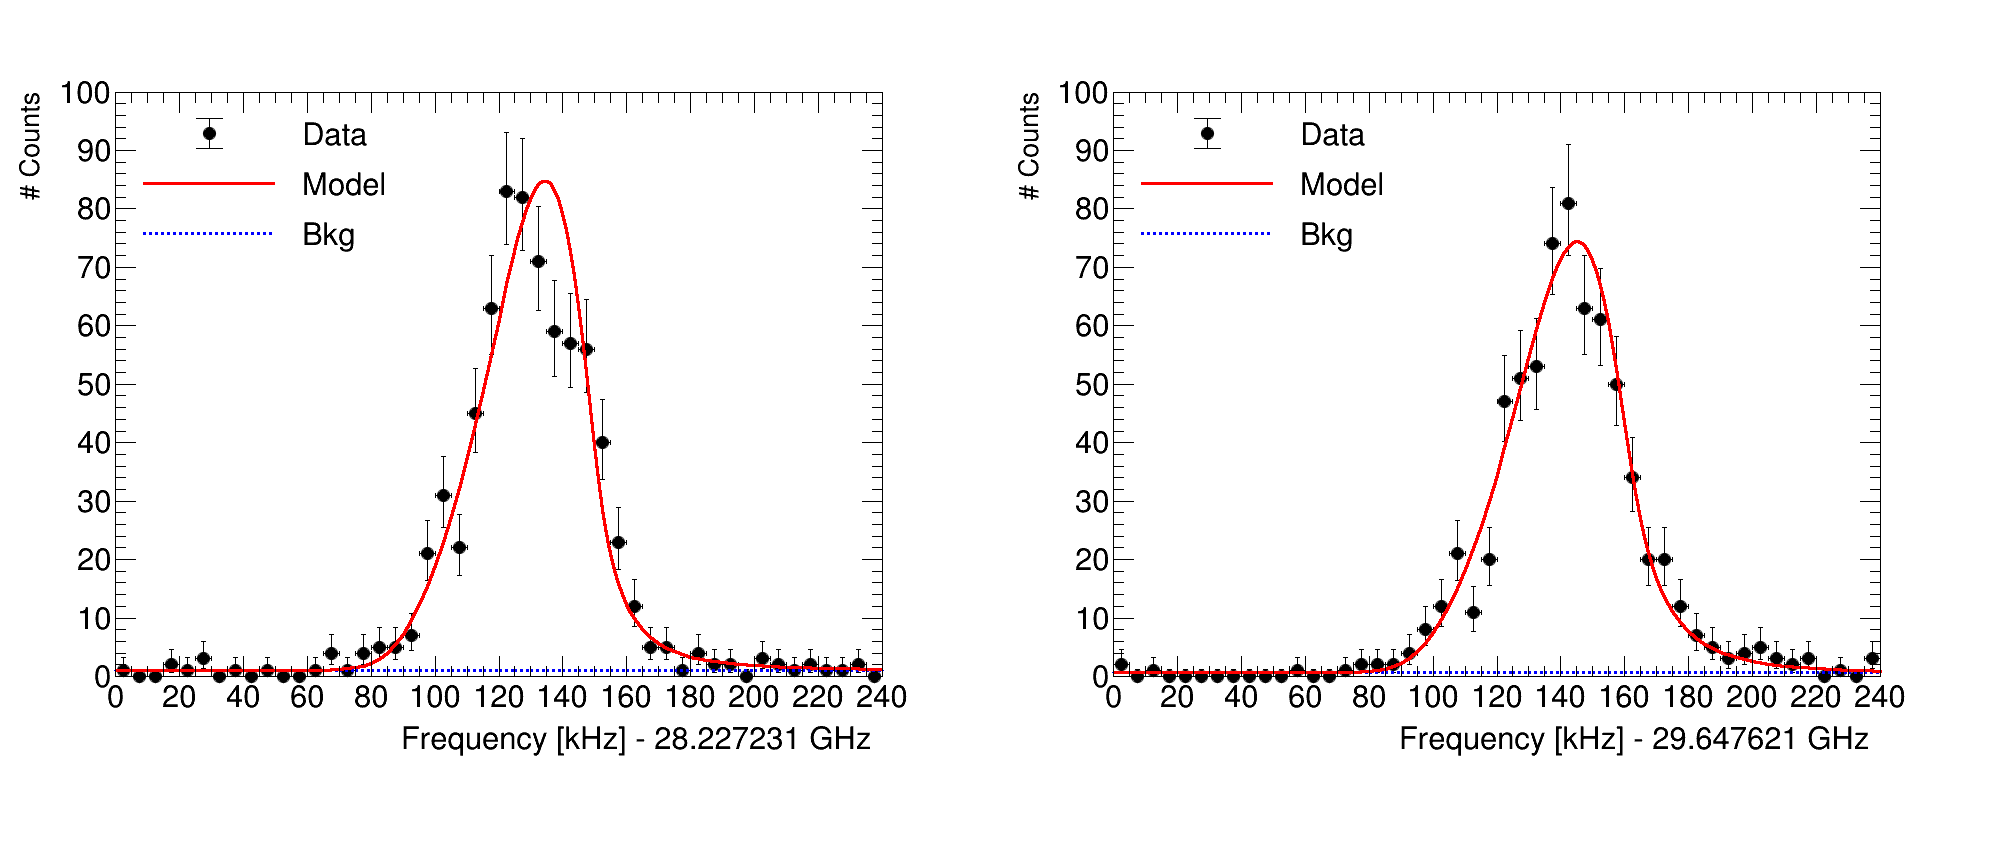
\includegraphics[width=\textwidth]{figures/chapter 4/Example-of-spectra.png}
\caption{Result of the maximum likelihood fit on repetition 3 for the set at \SI{1.03}{\tesla}.}
\label{fig:ExampleSpectra}
\end{figure}

\subsection{Blinding the Analysis}

The analysis was conducted blind to avoid bias during the development. A random offset $\delta f_{blinding}$ value was added to all frequency markers of the \da transition, applied uniformly across both datasets.

\begin{equation} \label{eq:deltaf}
f_{da}^{i} \equiv  f_{da}^{i} (t_{i}) +  \delta f_{blinding}
\end{equation}

Consequently, the hyperfine splitting extracted from both series was shifted by the same unknown quantity. This offset was revealed only when all the systematic uncertainties had been determined and a common consensus of the analysis procedure had been reached among ALPHA collaboration members.

Throughout this chapter the following convention is adopted. Absolute values of the hyperfine splitting quoted in tables (Tabs.~\ref{tab:results}, \ref{tab:selections}, \ref{tab:highstat_floatk}, \ref{tab:highstatparam}) are blind, and do not include the separation of \SI{1420390}{\kilo\hertz} between the \cb and \da sweeps. Quantities that are differences between analysis configurations ($\Delta$ columns, Tab.~\ref{tab:syst}), residuals and drift slopes (Tab.~\ref{tab:resultsBdrift}) do not depend on the blinding offset. Values quoted in full (e.g.\ $1\,420\,404.8$~kHz) are unblinded.

\subsection{Correlation between observables} \label{sec:Correlation}

The combined maximum likelihood estimation (MLE) approach, in which the model $f = g \otimes R$ of Eq.~\ref{eq:conv}, with the bare function $g$ of Eq.~\ref{eq:model1} and the resolution function $R$ of Eq.~\ref{GaussR}, is fitted simultaneously to all the repetitions of a series, offers several advantages. First, it reduces model complexity by allowing certain parameters to be shared across different datasets rather than fitted independently for each. Second, shape parameters like $\sigma_{rise}$ and $n_r$ benefit from the increased statistical power, as a consequence of being treated as global parameters. On the other hand, this approach introduces correlations between parameters, in particular the frequency markers, that must be carefully accounted for when deriving statistical uncertainties. Fig.~\ref{fig:CorrelationHeatMap} shows the correlation heat map of the MLE fit of the low-field series. As evident from the map, $\sigma_{cb}$ and $\sigma_{da}$, which control the onset shape of the spectra, are correlated with the frequency markers. This correlation arises because the shape parameters are constrained to be identical across repetitions, which in turn constrains the fitted frequency markers. The resulting covariance matrix of the frequency markers is reported in Tab.~\ref{tab:cov_matrix}.

\begin{figure}[!hbtp]
\centering
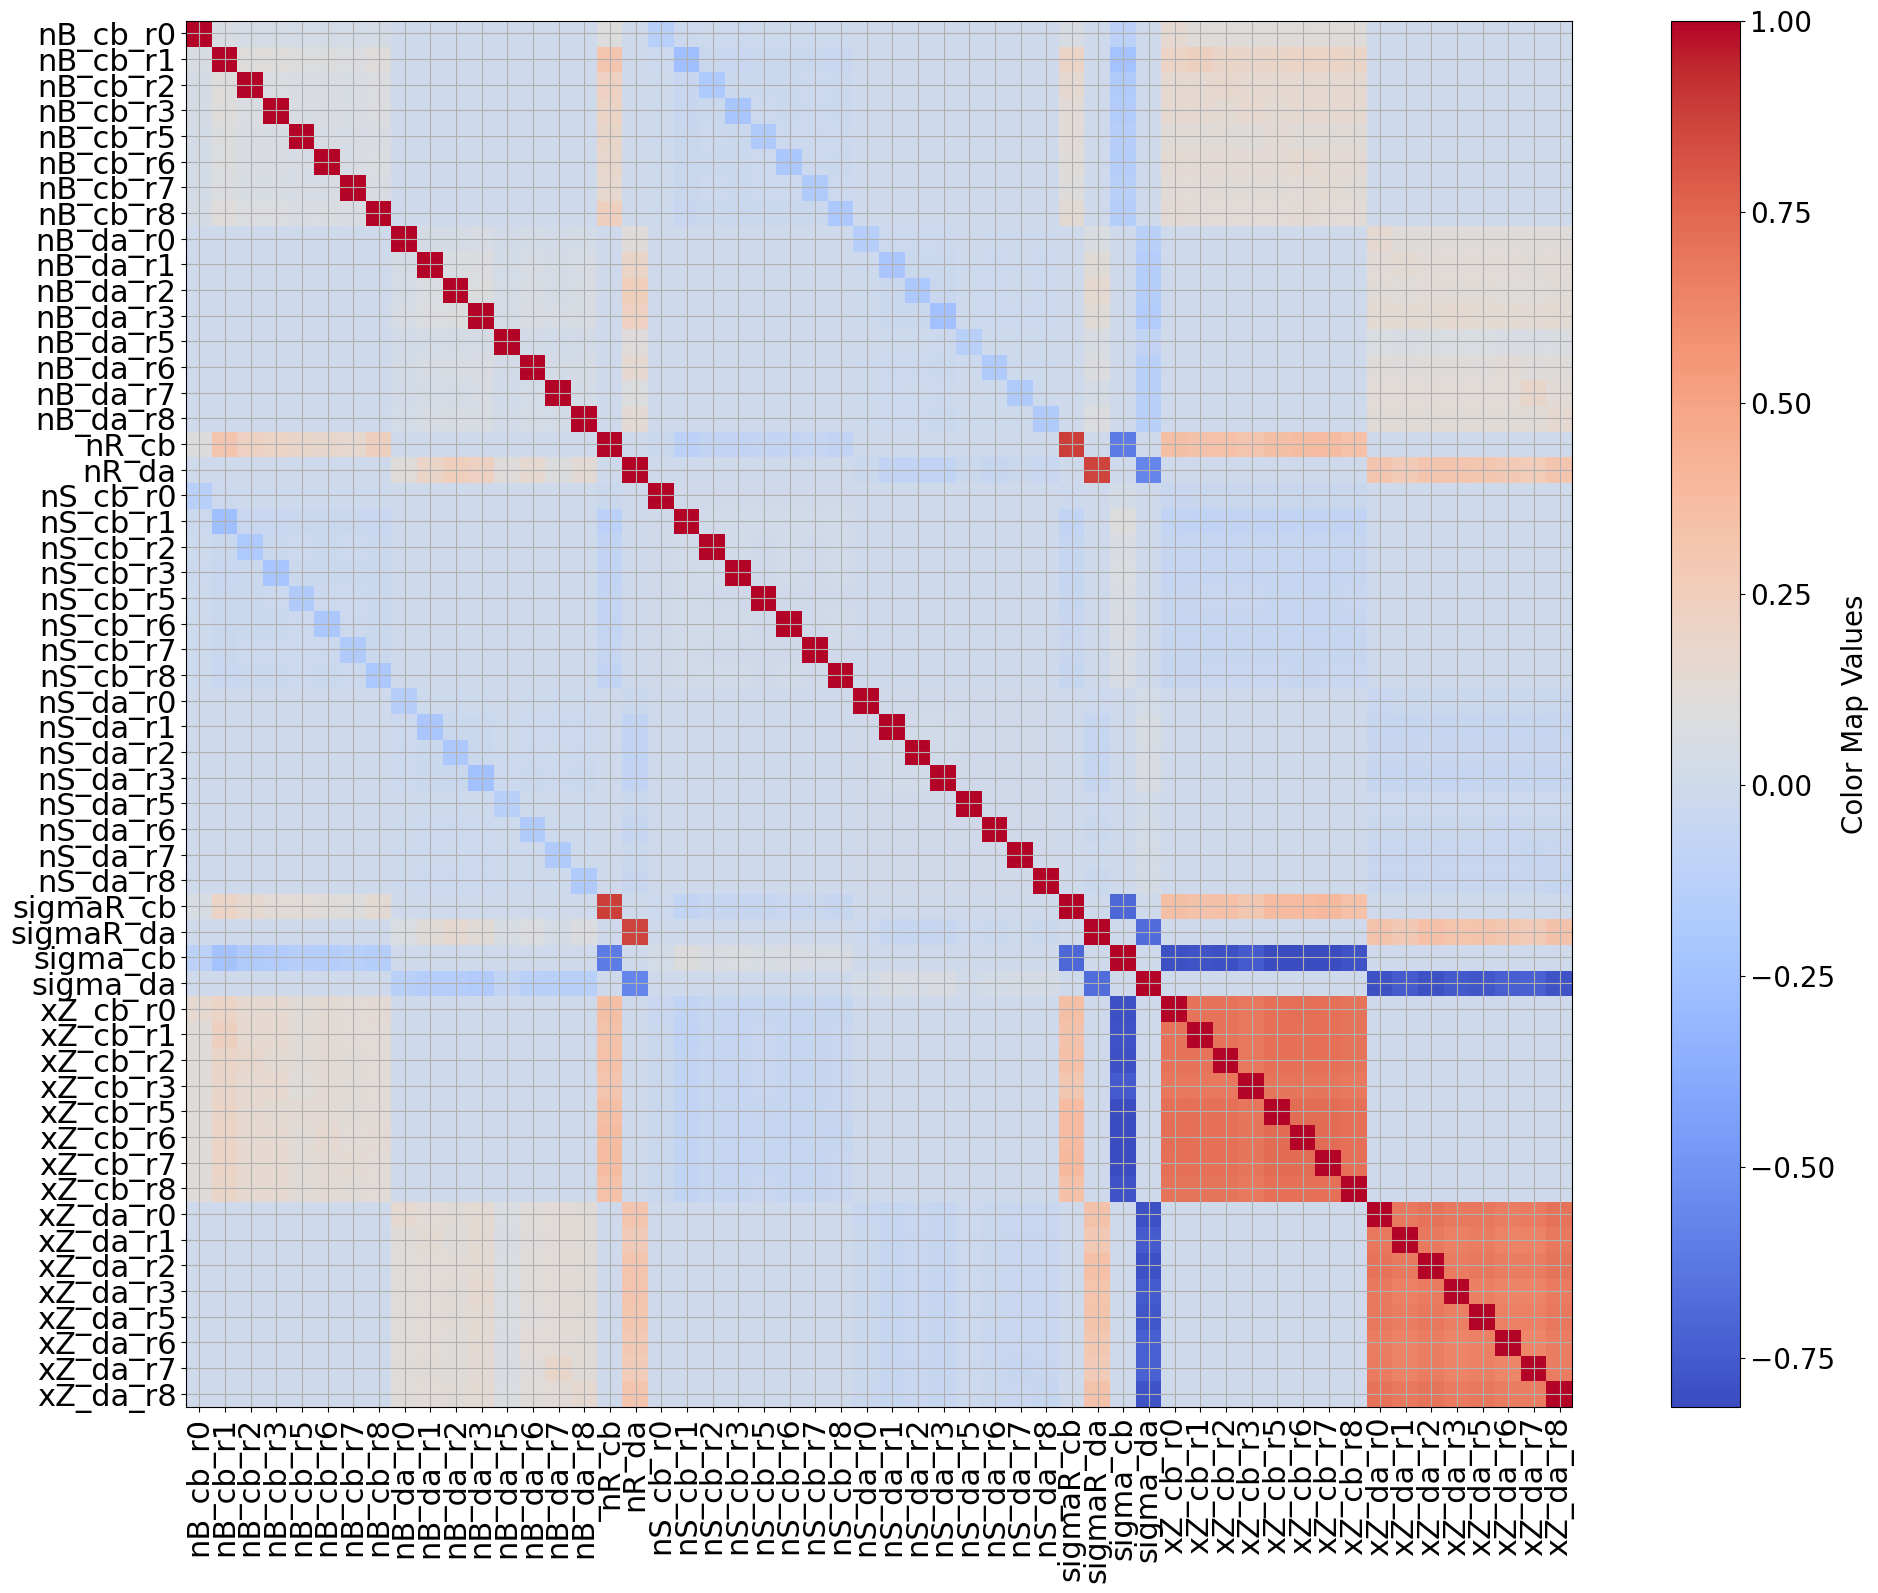
\includegraphics[width =  \textwidth]{figures/chapter 4/correlation_matrix_2026-05-28 102938_s8.png}
\caption{Correlation matrix of the MLE fit for the set of data at \SI{1.03}{\tesla}. The block of parameters labelled \texttt{xZ\_xx\_ry}, where \texttt{xx} denotes the transition (\texttt{cb} or \texttt{da}) and \texttt{y} the repetition number, corresponds to the frequency markers (the nomenclature used in the analysis code). The correlation of the frequency markers within the same transition is evident, as is their correlation with the shape parameter $\sigma_{xx}$. Correlations are also observed among other shape parameters $\sigma_{R,xx}$ and $n_{r,xx}$. These do not pose a problem since they influence the depletion tail of the spectrum, and are insensitive to the onset position.}
\label{fig:CorrelationHeatMap}
\end{figure}

\begin{table}[h]
    \centering
    \small 
    \scalebox{0.75}{
    \renewcommand{\arraystretch}{1.2}
    \begin{tabular}{l|cccccccc|cccccccc}
    \hline \hline
    & \multicolumn{8}{c|}{$f_{cb}$} & \multicolumn{8}{c}{$f_{da}$} \\
    \hline
\multirow{8}{*}{$f_{cb}$} & 2.23 & 1.36 & 1.34 & 1.41 & 1.40 & 1.40 & 1.31 & 1.40 & 0.00 & 0.00 & 0.00 & 0.00 & 0.00 & 0.00 & 0.00 & 0.00 \\
& 1.36 & 2.16 & 1.33 & 1.39 & 1.38 & 1.39 & 1.29 & 1.39 & 0.00 & 0.00 & 0.00 & 0.00 & 0.00 & 0.00 & 0.00 & 0.00 \\
& 1.34 & 1.33 & 2.23 & 1.38 & 1.37 & 1.38 & 1.29 & 1.38 & 0.00 & 0.00 & 0.00 & 0.00 & 0.00 & 0.00 & 0.00 & 0.00 \\
& 1.41 & 1.39 & 1.38 & 2.32 & 1.44 & 1.44 & 1.35 & 1.44 & 0.00 & 0.00 & 0.00 & 0.00 & 0.00 & 0.00 & 0.00 & 0.00 \\
& 1.40 & 1.38 & 1.37 & 1.44 & 2.37 & 1.43 & 1.33 & 1.43 & 0.00 & 0.00 & 0.00 & 0.00 & 0.00 & 0.00 & 0.00 & 0.00 \\
& 1.40 & 1.39 & 1.38 & 1.44 & 1.43 & 2.13 & 1.34 & 1.44 & 0.00 & 0.00 & 0.00 & 0.00 & 0.00 & 0.00 & 0.00 & 0.00 \\
& 1.31 & 1.29 & 1.29 & 1.35 & 1.33 & 1.34 & 2.11 & 1.34 & 0.00 & 0.00 & 0.00 & 0.00 & 0.00 & 0.00 & 0.00 & 0.00 \\
& 1.40 & 1.39 & 1.38 & 1.44 & 1.43 & 1.44 & 1.34 & 2.28 & 0.00 & 0.00 & 0.00 & 0.00 & 0.00 & 0.00 & 0.00 & 0.00 \\
\hline
\multirow{8}{*}{$f_{da}$} & 0.00 & 0.00 & 0.00 & 0.00 & 0.00 & 0.00 & 0.00 & 0.00 & 2.36 & 1.50 & 1.46 & 1.48 & 1.40 & 1.44 & 1.43 & 1.51 \\
& 0.00 & 0.00 & 0.00 & 0.00 & 0.00 & 0.00 & 0.00 & 0.00 & 1.50 & 2.04 & 1.39 & 1.41 & 1.33 & 1.37 & 1.36 & 1.44 \\
& 0.00 & 0.00 & 0.00 & 0.00 & 0.00 & 0.00 & 0.00 & 0.00 & 1.46 & 1.39 & 2.16 & 1.38 & 1.31 & 1.34 & 1.33 & 1.40 \\
& 0.00 & 0.00 & 0.00 & 0.00 & 0.00 & 0.00 & 0.00 & 0.00 & 1.48 & 1.41 & 1.38 & 2.14 & 1.32 & 1.36 & 1.34 & 1.42 \\
& 0.00 & 0.00 & 0.00 & 0.00 & 0.00 & 0.00 & 0.00 & 0.00 & 1.40 & 1.33 & 1.31 & 1.32 & 2.11 & 1.29 & 1.28 & 1.35 \\
& 0.00 & 0.00 & 0.00 & 0.00 & 0.00 & 0.00 & 0.00 & 0.00 & 1.44 & 1.37 & 1.34 & 1.36 & 1.29 & 1.88 & 1.31 & 1.39 \\
& 0.00 & 0.00 & 0.00 & 0.00 & 0.00 & 0.00 & 0.00 & 0.00 & 1.43 & 1.36 & 1.33 & 1.34 & 1.28 & 1.31 & 1.97 & 1.37 \\
& 0.00 & 0.00 & 0.00 & 0.00 & 0.00 & 0.00 & 0.00 & 0.00 & 1.51 & 1.44 & 1.40 & 1.42 & 1.35 & 1.39 & 1.37 & 2.16 \\
\hline
    \end{tabular}
    }
    \caption{Covariance matrix of the frequency markers. The values in the off-diagonal blocks are of the order of $10^{-4}$--$10^{-5}$; the values have been written with a precision of 2 decimal places.}
    \label{tab:cov_matrix}
\end{table}

\subsection{Maximum Likelihood Fit: Results}

The results of the nominal maximum likelihood fit for the two series are summarized in Tab.~\ref{tab:resultsf0}. Two parameters are kept fixed in the nominal configuration: the width of the one-sided Gaussian resolution function, $t_{gauss} = \SI{10}{\kilo\hertz}$ for both transitions, obtained from the fit to the simulations (Sec.~\ref{sec:Simulation}), and the degree of the power-law rise, $k=2$. The shape parameters of the bare function $g$ ($n$, $\sigma$, $\sigma_r$) are shared among the eight repetitions of the same transition, but are determined separately for the \cb and \da transitions. The table also reports the corresponding rise length $r = \sigma (k+1)$, i.e.\ the distance between the onset and the maximum of the lineshape, and the sixteen frequency markers of each series, one for each repetition and transition. Since each spectrum is fitted after setting the first frequency of its scan to zero, the markers are expressed relative to the initial frequency of the corresponding scan; the initial frequencies of the \cb and \da scans of the same repetition are separated by \SI{1420390}{\kilo\hertz} (Tab.~\ref{tab:ListOfRuns}). The \da markers are reported after unblinding, i.e.\ with $\delta f_{blinding} = 0$.

Some features of the results are worth noting. The parameters that control the onset region of the lineshape are very similar for the two transitions: $\sigma$ is about \SI{19}{\kilo\hertz} in the high-field series and \SIrange{20}{21}{\kilo\hertz} in the low-field series, and the rise lengths of the \cb and \da transitions agree within about one standard deviation in both series. This indicates that the balancing of the microwave power between the two transitions (Sec.~\ref{sec:MWpower}) was effective where it matters most, since the onset region is the part of the spectrum that determines the frequency markers. Larger differences between the two transitions are found in $\sigma_r$ and $n$, which describe the depletion tail of the lineshape and, as discussed in Sec.~\ref{sec:Correlation}, are only weakly correlated with the frequency markers. The statistical uncertainty of each marker is \SIrange{1.2}{1.5}{\kilo\hertz}; part of it comes from the shared shape parameters, which also produce the correlations between the markers of the same transition shown in Tab.~\ref{tab:cov_matrix}.

The markers change from one repetition to the next, since the initial frequency of each scan is set according to the expected magnetic field drift (Fig.~\ref{fig:RepetitionScheme}), and the actual drift differs from the expected one. Moreover, the \da scan starts about \SI{812}{\second} after the \cb scan of the same repetition, during which the magnetic field keeps decaying. For these reasons, the difference $f_{o,da}^{(i)} - f_{o,cb}^{(i)}$ of a single repetition is not directly an estimate of the hyperfine splitting: the markers must first be corrected for the magnetic field drift, as described in the next section.

% TABLE 6 - RESULTS
\begin{table}[!h]
\centering
\begin{tabular}{l|cc}
\hline
\hline
\textbf{} & \textbf{\SI{1.07}{\tesla} (high field)}  &  \textbf{\SI{1.03}{\tesla} (low field)}  \\
\hline 
$t_{gauss}^{(cb)}$ (kHz) (fixed) & $10$ & $10$ \\
$t_{gauss}^{(da)}$ (kHz) (fixed) & $10$ & $10$ \\
%$t_R$ (kHz) (fixed) & $0.2$& $0.2$ \\
\hline
$k$ (fixed) &  $2$ &  $2$ \\
$n^{(cb)}$                &  $ 10 \pm 6$	         & $ 3.4    \pm 0.8 $\\
$n^{(da)}$                &  $\phantom{0}6  \pm 2$   & $  4.7   \pm 1.3 $\\
$\sigma^{(cb)}$ (kHz)     &  $	19.2 \pm 0.7  $      & $ 20.3   \pm 0.6 $\\
$\sigma^{(da)}$ (kHz)     &  $	19.1 \pm 0.7  $      & $ 21.1  \pm 0.6 $\\
$\sigma^{(cb)}_{r}$ (kHz) & $	15.0 \pm 1.0 $       & $ 6.2    \pm 0.6  $\\
$\sigma^{(da)}_{r}$ (kHz) & $	10.9 \pm 0.7  $      & $ 8.7    \pm 0.7  $\\
\hline
rise $r_{cb}$             & $ 57.6 \pm 2.07$         & $ 60.8 \pm 1.63$ \\ 
rise $r_{da}$             & $ 57.4 \pm 1.98$          & $ 63.2 \pm 1.68$ \\
\hline
$f_{o,cb}^{(0)}$ (kHz) &   $ 140.3 \pm 1.5 $ & $ 120.1 \pm 1.2 $ \\
$f_{o,cb}^{(1)}$ (kHz) &   $ 106.0 \pm 1.5 $ & $ 93.7 \pm 1.2 $ \\
$f_{o,cb}^{(2)}$ (kHz) &   $ 100.9 \pm 1.5 $ & $ 89.4 \pm 1.2 $ \\
$f_{o,cb}^{(3)}$ (kHz) &   $ 92.7 \pm 1.5 $ & $ 86.1 \pm 1.2 $ \\
$f_{o,cb}^{(4)}$ (kHz) &   $ 92.8 \pm 1.5 $ & $ 103.0 \pm 1.2 $ \\
$f_{o,cb}^{(5)}$ (kHz) &   $ 95.9 \pm 1.5 $ & $ 107.7 \pm 1.2 $ \\
$f_{o,cb}^{(6)}$ (kHz) &   $ 100.6 \pm 1.5 $ & $ 117.1 \pm 1.2 $ \\
$f_{o,cb}^{(7)}$ (kHz) &  $ 99.1 \pm 1.5 $ & $ 113.5 \pm 1.2 $ \\ 
\hline
$f_{o,da}^{(0)}$ (kHz) & $ 139.6 \pm 1.5 $ & $ 112.0 \pm 1.2 $ \\
$f_{o,da}^{(1)}$ (kHz) & $ 104.1 \pm 1.4 $ & $ 88.7 \pm 1.3 $ \\
$f_{o,da}^{(2)}$ (kHz) & $ 96.7 \pm 1.5 $ & $ 84.3 \pm 1.3 $ \\
$f_{o,da}^{(3)}$ (kHz) & $ 84.7 \pm 1.5 $ & $ 93.4 \pm 1.3 $ \\
$f_{o,da}^{(4)}$ (kHz) & $ 96.4 \pm 1.5 $ & $ 102.0 \pm 1.2 $ \\
$f_{o,da}^{(5)}$ (kHz) & $ 93.4 \pm 1.4 $ & $ 101.6 \pm 1.3 $ \\
$f_{o,da}^{(6)}$ (kHz) & $ 94.0 \pm 1.4 $ & $ 120.6 \pm 1.2 $ \\
$f_{o,da}^{(7)}$ (kHz) & $ 87.6 \pm 1.5 $ & $ 108.2 \pm 1.3 $ \\
\nullo{\hline
$\Delta f^{(i)} = f^{(i)}_{o,da} - f^{(i)}_{o,cb}$ & &      \\
$\Delta f^{(0)}$ (kHz)  & -5.4 $\pm$ 2.1 & -12.9 $\pm$ 1.7  \\
$\Delta f^{(1)}$ (kHz) & -6.6 $\pm$ 2.1 & -9.8 $\pm$ 1.7    \\
$\Delta f^{(2)}$ (kHz)  & -9.0 $\pm$ 2.1 & -9.9 $\pm$ 1.8   \\
$\Delta f^{(3)}$ (kHz) & -12.7 $\pm$ 2.1 & 2.6 $\pm$ 1.7    \\
$\Delta f^{(4)}$ (kHz)  & -1.2 $\pm$ 2.1 & -5.8 $\pm$ 1.8   \\
$\Delta f^{(5)}$ (kHz) & -7.2 $\pm$ 2.0 & -10.8 $\pm$ 1.8   \\
$\Delta f^{(6)}$ (kHz) & -11.3 $\pm$ 2.0 & -1.2 $\pm$ 1.8   \\
$\Delta f^{(7)}$ (kHz)  & -16.3 $\pm$ 2.1 & -10.0 $\pm$ 1.7 \\}
\hline 
\hline
\end{tabular}
\caption{Results (parameters and frequency markers) of the nominal maximum likelihood fit. All the values for $f_{o,da/cb}^{(i)}$ are reported with respect to the start frequency of the corresponding transition scan.
\label{tab:resultsf0}}
\end{table}

\section{Magnetic Field Drift}

In Sec.~\ref{Protocol-of-experiment} we have introduced an important effect that requires treatment in the analysis: the decay of the bias (Carlsberg) magnetic field during the course of the experiment. Due to the delay of the measurement for the higher-frequency transition in each repetition, a correction must be applied. In the analysis it is assumed that the magnetic field decay acts linearly, and with the same slope value, for the two transitions. Hence, the two sets of 8 frequencies plotted versus time will lie on two parallel lines. As a consequence, it is possible to derive a correction associated with the field decay from a linear fit to the frequency markers. The linearity assumption has been relaxed: a different approach has been followed to estimate deviations from linearity, using GPR \footnote{GPR: Gaussian Process Regressor} interpolation, only assuming that the hyperfine splitting for antihydrogen does not depend on the bias field in the range of this measurement campaign. More details are given in Sec.~\ref{sec:decaySystematic}.

In terms of frequency markers, the hyperfine splitting is given by

\begin{equation}
a_{1S}/h = f_{da}^{i}(t) - f_{cb}^{i}(t) =  f_{da}^{i}(t + \Delta_t) - m \Delta_t - f_{cb}^{i}(t)
\end{equation}

where $\Delta_t$ is the time interval that occurs between a \cb and the following \da transition.


\subsection{Extended Least Square Minimization} \label{sec:CommonFitExtraction}

%Assuming the same linear drift of the transition frequency as a function of time, resulting from the decay of the magnetic field of the solenoid, a common fit to the 8 $f_{o,cb}^{(i)}$ and $f_{o,da}^{(i)}$ gives the value of the blind $a^{blind}_{1S}/h$ and of the common linear drift $m$.
%The nominal procedure assumes the decay of the solenoidal magnetic field to be linear in time and equal for the two transitions. 
The hyperfine splitting $a_{1S}/h$ is extracted with a linear fit to the 8 \cb and 8 \da frequency markers (after having set $f_{blinding}$ to 0), imposing a common slope for both transitions.

As can be noted from the correlation matrix reported in Tab.~\ref{tab:cov_matrix}, the frequency markers, which correspond to the $y_{i}$ observables, are correlated with each other, due to the presence of shared parameters in the combined fit to the repetition datasets.
The algorithm used for the linear fit is the Generalized Least Squares (GLS), a generalization of the ordinary least squares algorithm. This generalization is necessary to properly account for correlations. The linear model can be expressed as:

\begin{equation}
    \vec{y} = \vec{\beta} \; {\bf X} + \vec{\epsilon}
\end{equation}

where the ${\bf X}$ matrix contains the time of each repetition; $\beta$ is the fit parameter vector, $\epsilon$ is the error vector of the $y_{i}$ observables, which is described by the covariance matrix $\Omega$ reported in Tab.~\ref{tab:cov_matrix}. 

The above equation can be explicitly written in matrix form, to highlight the arrangement of the variables for the combined fit procedure:

\begin{gather}
\begin{bmatrix}
f_{cb}^{0} \\
f_{cb}^{1} \\
\vdots     \\
f_{da}^{0} \\
f_{da}^{1} \\
\vdots
\end{bmatrix} =
\begin{bmatrix}
    1        & -0.5   & t_{cb}^{0}    \\
    1        & -0.5   & t_{cb}^{1}    \\
    \vdots   & \vdots & \vdots      \\
    1        & +0.5   &  t_{da}^{0} \\
    1        & +0.5   &  t_{da}^{1} \\
    \vdots   & \vdots & \vdots
\end{bmatrix} \times
\begin{bmatrix}
    q   \\
    a_{1S}/h \\
    m
\end{bmatrix}
\end{gather}

Where $f^{i}$ are the frequency markers, and $t^{i}$ the time at which an onset of each transition is identified. For the \da onset:

\begin{equation}
t^{i}_{da,cb} = t_{start \; sweep} + j \cdot 8s  
\end{equation}

where the time is corrected for the $j$-th bin of the scan where the frequency marker is found. Given this linear system of equation, the solution of this regression problem is given by the following equation, whose derivation is omitted \cite{Aitken1935}:

\begin{align}
    \vec{\beta} &= ({\bf X^{T}} \Omega^{-1} {\bf X})^{-1} {\bf X^{T}} \Omega^{-1}\vec{y} \\
    \sigma^{2}_{\beta} &= ({\bf X^{T}} \Omega^{-1} {\bf X})^{-1}
\end{align}

This solution, for the linear case, can be written directly in a closed form. This was the final version that has been used to correct for the magnetic field drift over time. The results of the fit are reported in Fig.~\ref{fig:FitEOLS}.

\begin{figure}[!htbp]
\centering
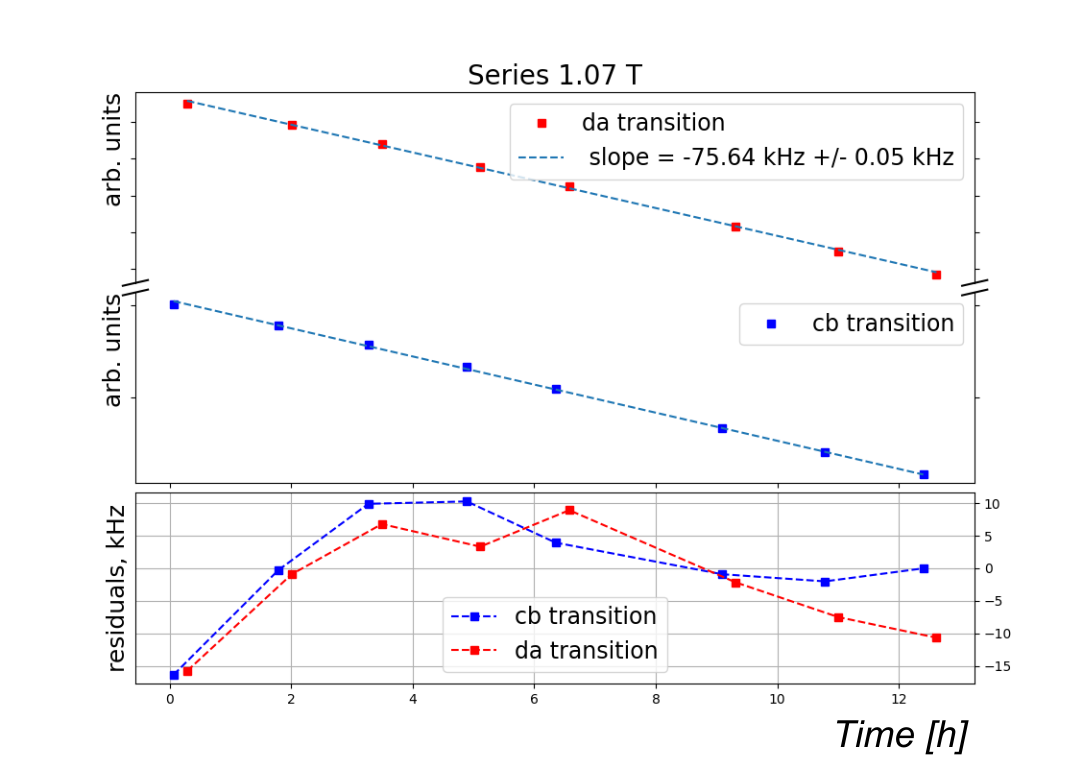
\includegraphics[width = 0.95\textwidth]{figures/chapter 4/cb_da_time_s7.png} \\
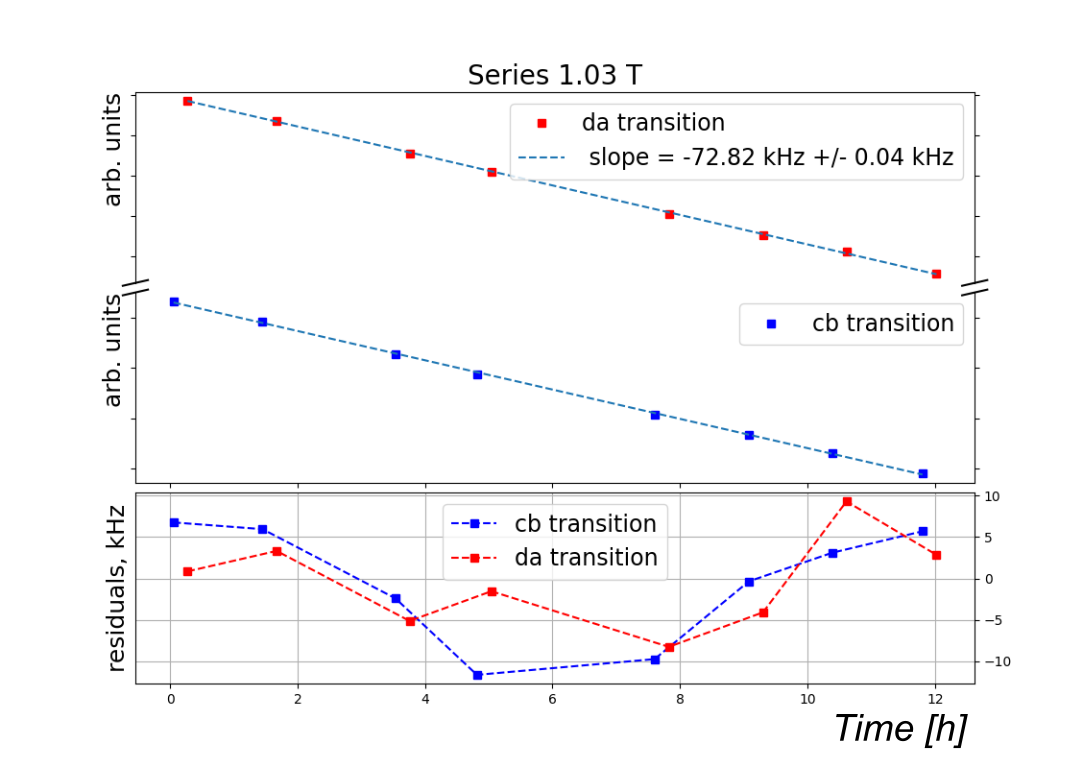
\includegraphics[width = 0.95\textwidth]{figures/chapter 4/cb_da_time_s8.png}
\caption{Frequency markers versus time for the \cb and \da transition of the high field (top) and low field (bottom) series. The blue dotted line is the extended least square fit with common slope between the two lines.}
\label{fig:FitEOLS}
\end{figure}

The plots shown in the previous figure also contain the non-normalized residuals of the linear extraction. The residuals for each individual run are also reported in Tab.~\ref{tab:resultsBdrift}, and are simply defined as: 

\begin{equation}
res_{i} = f^{i}_{cb/da}(t_{i}) - ( m_{common} * t_{i} + q \pm \frac{a_{1S}}{2h})
\end{equation}

The statistical uncertainty associated with each $f^{i}_{cb/da}$ is of order \SI{1}{\kilo \hertz}. The dispersion of the residuals around zero is not compatible with 1 standard deviation. This should not, however, be interpreted as an argument against the analysis, since the effect that certain systematics have on the position of the frequency markers has not been taken into account. In the next section, a comprehensive review of the main systematic uncertainties associated with the experimental campaign and the analysis technique is presented.

\section{Systematic Uncertainties}

This section contains a detailed explanation of each systematic uncertainty source of the ground state hyperfine splitting of the antihydrogen atom measured at ALPHA.
The systematic uncertainties have been derived mainly with a data-driven approach, which could be explained as ``what would be the result of the analysis if an alternative choice had been made?''. By looking at the discrepancies between the alternative choice and the nominal one, a systematic uncertainty is quoted. 

The measurement is affected by multiple systematic sources. Some arise from the analysis and extrapolation procedure itself (e.g., magnetic-field-drift correction, binning choices, data selection), while others are linked to properties of the data, such as lineshape variations between repetitions or between the \cb and \da transitions. Although the two transitions were equalized by tuning the applied microwave power, a residual lineshape difference remains and is included in the uncertainty budget.

As noted earlier, the key physical observable is extracted by difference: the resonance frequencies of the two transitions are not determined independently. Instead, the analysis uses fitted frequency markers—model parameters that act as proxies for resonance positions, without requiring them to be individually unbiased estimators of the true resonance frequencies. This differential strategy suppresses or cancels several systematic contributions and enables a precise measurement even in the absence of a fully realistic physical simulation of the spectra.

\subsection{The bare function \texorpdfstring{$g$}{g}}

This section contains a summary of the systematic uncertainties related to the signal model (before introducing the convolution with the asymmetric resolution function). A systematic uncertainty has been associated to the parameters controlling the signal shape, and the function choice itself.

\subsubsection{Parameters controlling the signal shape}
The shape parameters obtained from the fit to simulation, which rules the power law rise and the broadening, are used in the nominal MLE fit to extract the hyperfine splitting. However, since the simulation does not have the complete physics to fully describe the spectra, a simultaneous fit to the available high-statistics sample was performed, to benchmark the result of the simulation and to evaluate systematic uncertainty associated with the fixed parameters used in the nominal procedure.

High-statistics samples consist of runs collected with much greater stacking of atoms than the standard runs; they are used exclusively to fix certain parameters of the model and are not included in the extraction of the physics results. A total of three high-statistic repetitions were acquired: two of them for low magnetic field series (one before and one after the 8 repetitions) and one for the high field series (taken after the 8 nominal repetitions).

The high-statistics samples have been fitted with the same empirical model described above. The aim is to get an estimation from the data of the shape parameters, in particular $k$, the degree of the power law rise, in order to use that value as an alternative way in the nominal fit to extract the hyperfine splitting. The absolute difference between the nominal extracted value and the alternative analysis with $k$ is then used to quote the systematic uncertainty. Because of this, $k$ is a free parameter, shared among all the high-statistics samples. Instead of minimizing the frequency markers individually (using $f_{cb}$ and $f_{da}$ as free parameters), the fit was varied with the intention of fitting $f_{cb}$ and the splitting itself $\Delta_f$, such that the $f_{da} = f_{cb} + \Delta_f$. By doing so, it is possible to impose a common splitting between the three high-statistics repetitions too. The results of the fit are shown in Tab.~\ref{tab:highstat_floatk}, while the plot in Fig.~\ref{fig:fitwithfloatingk} shows the fit model and data.

%Minuit2Minimizer : Valid minimum - status = 0
%FVAL  = 263.837229792095229
%Edm   = 0.00086527296112601476
%Nfcn  = 11477
\begin{table}[!h]
\centering
\resizebox{\columnwidth}{!}{
\begin{tabular}{l|ccc}
\hline
\hline
\textbf{}   & \textbf{\SI{1.07}{\tesla} post}  & \textbf{\SI{1.03}{\tesla} pre}  &  \textbf{\SI{1.03}{\tesla} post}  \\
\hline 
$k$ (common)                        & \multicolumn{3}{c}{    $5.4 \pm 0.2$ }\\
$n^{(cb)}$ (common)    & \multicolumn{3}{c}{    $7.3 \pm 2.4$ }\\
$n^{(da)}$ (common) & \multicolumn{3}{c}{    $6.3 \pm 1.6$ }\\
$\sigma^{(cb)}$ (kHz)      & $17.0 \pm  0.8$  & $ 15.1 \pm 0.5  $ & $15.9 \pm 0.5$  \\
$\sigma^{(da)}$ (kHz)      & $15.8 \pm 0.7$   & $ 15.7 \pm 0.5  $ & $17.6 \pm 0.5$  \\
$\sigma^{(cb)}_{r}$ (kHz)  & $14.3 \pm  1.0$  & $ 8.9 \pm 0.6  $  & $8.7 \pm 0.6$  \\
$\sigma^{(da)}_{r}$ (kHz)  & $12.2 \pm  0.8$  & $ 11.2 \pm 0.7  $ & $9.9 \pm 0.7$  \\
$n_B^{(cb)}$               &  $ 150 \pm 22$   & $  109 \pm 20  $  &  $ 33 \pm 11$ \\
$n_B^{(da)}$               &  $ 80 \pm 16$    & $  83 \pm 21 $    &  $ 62 \pm 14$  \\
$n_S^{(cb)}$               &  $ 2271 \pm 48$  & $  2687 \pm 53  $ &  $ 2705\pm 52$ \\
$n_S^{(da)}$               &  $ 2221 \pm 48$  & $  2724 \pm 54  $ &  $ 2724\pm 52$ \\
\hline
%xZ_cb_post	  = 70.1359	 +/-  3.36124	(limited)
%xZ_cb_pre	  = 31.5012	 +/-  3.12625	(limited)
%xZ_cb_pst7	  = 47.503	 +/-  3.64418	(limited)
$\Delta f$ (kHz)           & \multicolumn{3}{c}{$ -12.7  \pm 2.8$}\\
\hline\hline
time from center of associated series (h) & $11.5$ & $-7$ & $11.2$ \\
duration of associated series (h)         & $12$ & $11.75$ & $11.75$\\
\hline
\hline
\end{tabular}
}
\caption{Model float parameters from the high-statistics samples. \label{tab:highstat_floatk}}
\end{table}

The $k$ result of the fit is 5.4, which has been used to evaluate a component of the systematic uncertainty associated with function shape variation. Since those data have been used for this task, they are not included in the main analysis, which relies only on the eight repetitions with less statistical power. 

The value of $k$ has been varied within a range whose extremes are given by the fits to the simulations and to the high-statistics samples. The nominal value $k=2$ is based on the fits to the simulations (Sec.~\ref{sec:Simulation} and Tab.~\ref{tab:resfun}). The lower extreme, $k=1$, corresponds to the lower values of $k$ obtained from the fits to the 2024 simulations ($k = 1.23 \pm 0.3$) and with the cusp resolution function, while the upper extreme, $k=5.4$, is the value obtained from the high-statistics samples. The parameter $k$ drives the extrapolation of the frequency marker: the higher its value, the further the frequency marker is from the maximum of the bare function $g$, and the larger its uncertainty, because of the longer extrapolation arm. When evaluating the systematic uncertainty associated with a larger value of $k$, this is taken into account by an additional contribution
\begin{equation}
\sigma_{syst,k} = \sqrt{\sigma^{2}_{k} - \sigma^{2}_{nominal}} \, ,
\end{equation}
where $\sigma_{k}$ and $\sigma_{nominal}$ are the statistical uncertainties of the hyperfine splitting obtained with $k = 5.4$ and with the nominal value, respectively. The results obtained with $k=1$ and $k=5.4$, together with this contribution (row \textit{max uncertainty increase}), are reported in Tab.~\ref{tab:results}, in the block \textit{bare function $g$ (parameters)}.

\begin{figure}[!htbp]
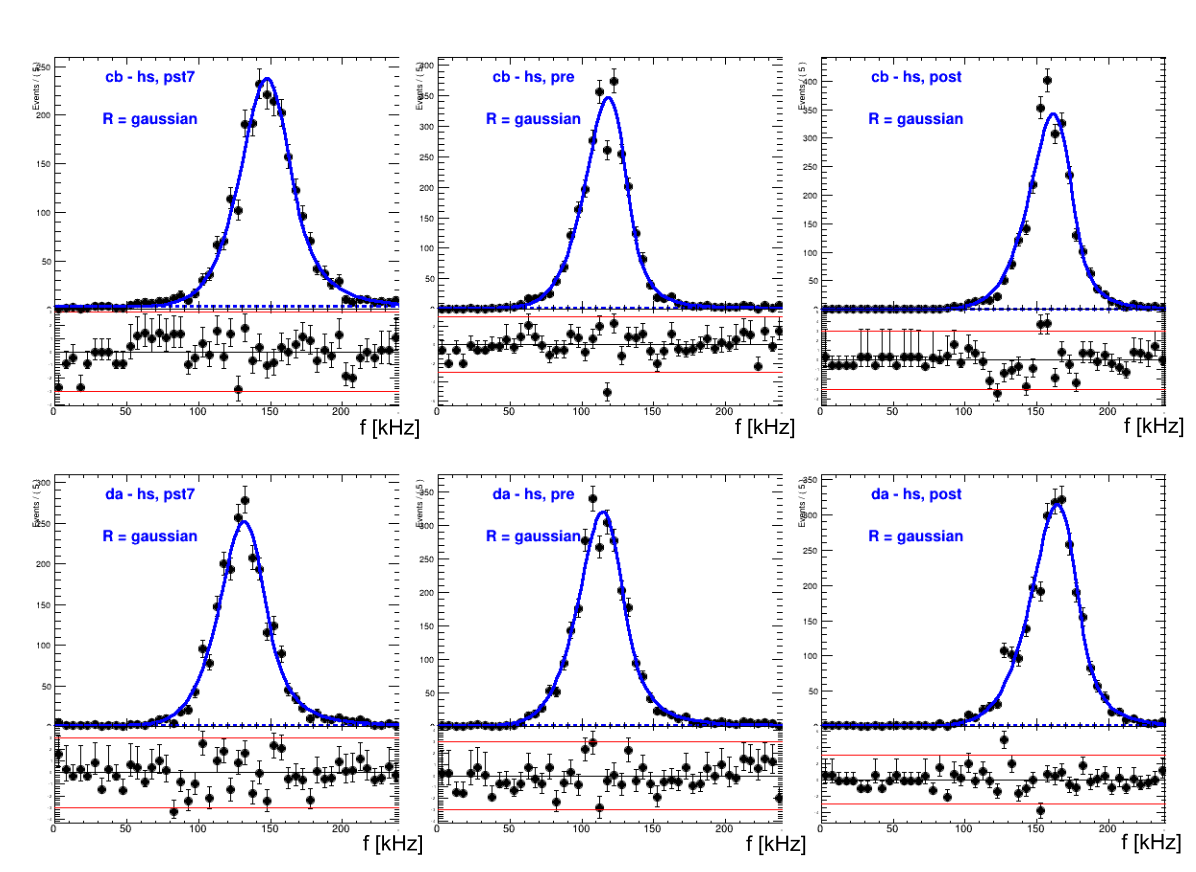
\includegraphics[width=\textwidth]{figures/chapter 4/highstat_kfloat.png}
\caption{Fit results on the high-statistics samples, with the shared $k$ parameter left free to vary in the fit, and with shared $\Delta f$, to help the convergence of the fit.}
\label{fig:fitwithfloatingk}
\end{figure}

\subsection{Alternative bare function}

An alternative function has been used to evaluate systematic uncertainty about the choice of the bare function $g$. The mathematical form of the model is:

\begin{equation}
\begin{dcases}
0 \quad \overline{x} < 0 \\
\left(\frac{\overline{x}}{\sigma}\right)^k \text{exp}\left( - \left(\frac{\overline{x}}{\sigma}\right)^{k+1} \frac{\sigma}{\sigma_r}  \frac{1}{k + 1}\right) \quad 0 \leq \overline{x} \land  \overline{x} \leq \sigma  \\
\text{exp}( \frac{\sigma}{\sigma_r} \left( \frac{k}{k+1}\right) \times \text{exp}(-\frac{\overline(x)}{\sigma_r}) \quad (\overline{x} \geq \sigma)
\end{dcases}
\end{equation}

 This model was originally developed to describe Monte Carlo simulations designed for an earlier version of the experiment, and it was deemed a suitable choice for validating the nominal empirical model. Its formulation, similarly to the nominal empirical model, was not derived rigorously from first-principles theoretical physics, but rather in a semi-empirical way.
The model considers a continuous rather than a stepped frequency ramp, and here $N_0$ is the number of trapped anti-atoms, $t_0$ is the time at which the onset condition is met, $\tau$ is the depletion rate during irradiation, and $T_{ramp}$ is the time between the onset and the peak \commento{mi sembra sia così nel modello}, and $\lambda$ controls the shape. The systematic uncertainty has been evaluated by repeating the full analysis routine with this alternative function and considering the shift in the final result compared to the nominal choice (similarly to what has been done for the majority of the systematics). The result is reported in Tab.~\ref{tab:results}, in the block \textit{bare function $g$ (choice)}.

\subsection{Frequency marker systematic uncertainty: the resolution function}

In Secs.~\ref{sec:resolutionF} and \ref{sec:Simulation} we introduced several mechanisms that broaden the observed lineshapes beyond the natural linewidth. The main contributions include magnetic-field inhomogeneity and oscillations, Doppler broadening, transit-time broadening, and microwave frequency instability. These effects are crucial because they directly affect the definition of the frequency marker.
 
A first-principles evaluation of each contribution is challenging, as it would require full knowledge of the trap dynamics, which is not available. Therefore, the approach was to vary the resolution function, both its functional form and its parameters, in order to estimate the associated systematic uncertainty on the hyperfine splitting. As a reminder, the systematic uncertainty is not linked to our ignorance of the real position of the resonance frequency given a certain transition shape. As stated before, the physical quantity is obtained through a measurement by difference, hence any point in the shape could in principle be used as a frequency marker. What really determines the accuracy of the measurement is that this frequency marker must be the same for the \cb and \da transitions. Any systematic difference in the shape of the transition directly changes the frequency marker and hence the measured splitting. In conclusion, since what matters most is the relative difference between the two transitions, this will reflect the way we have computed this systematic uncertainty.

The broadening scale, which sets the width of the resolution function, was extracted by fitting the available simulation data (see Figs.~\ref{fig:sim2023} and \ref{fig:sim2024}). Multiple spectra were simulated for different amplitudes of the microwave field in the trap cavity and analyzed using the same empirical model used for the experimental dataset. Since the onset (i.e., the transition starting point) is an input parameter of the simulation (and is placed at zero in all the simulations), it was fixed to its known value and treated as a constant. In contrast, the broadening amplitude $t_{gauss}$ and $t_{cusp}$ were left as free parameters.

\begin{sidewaysfigure}[hp]
    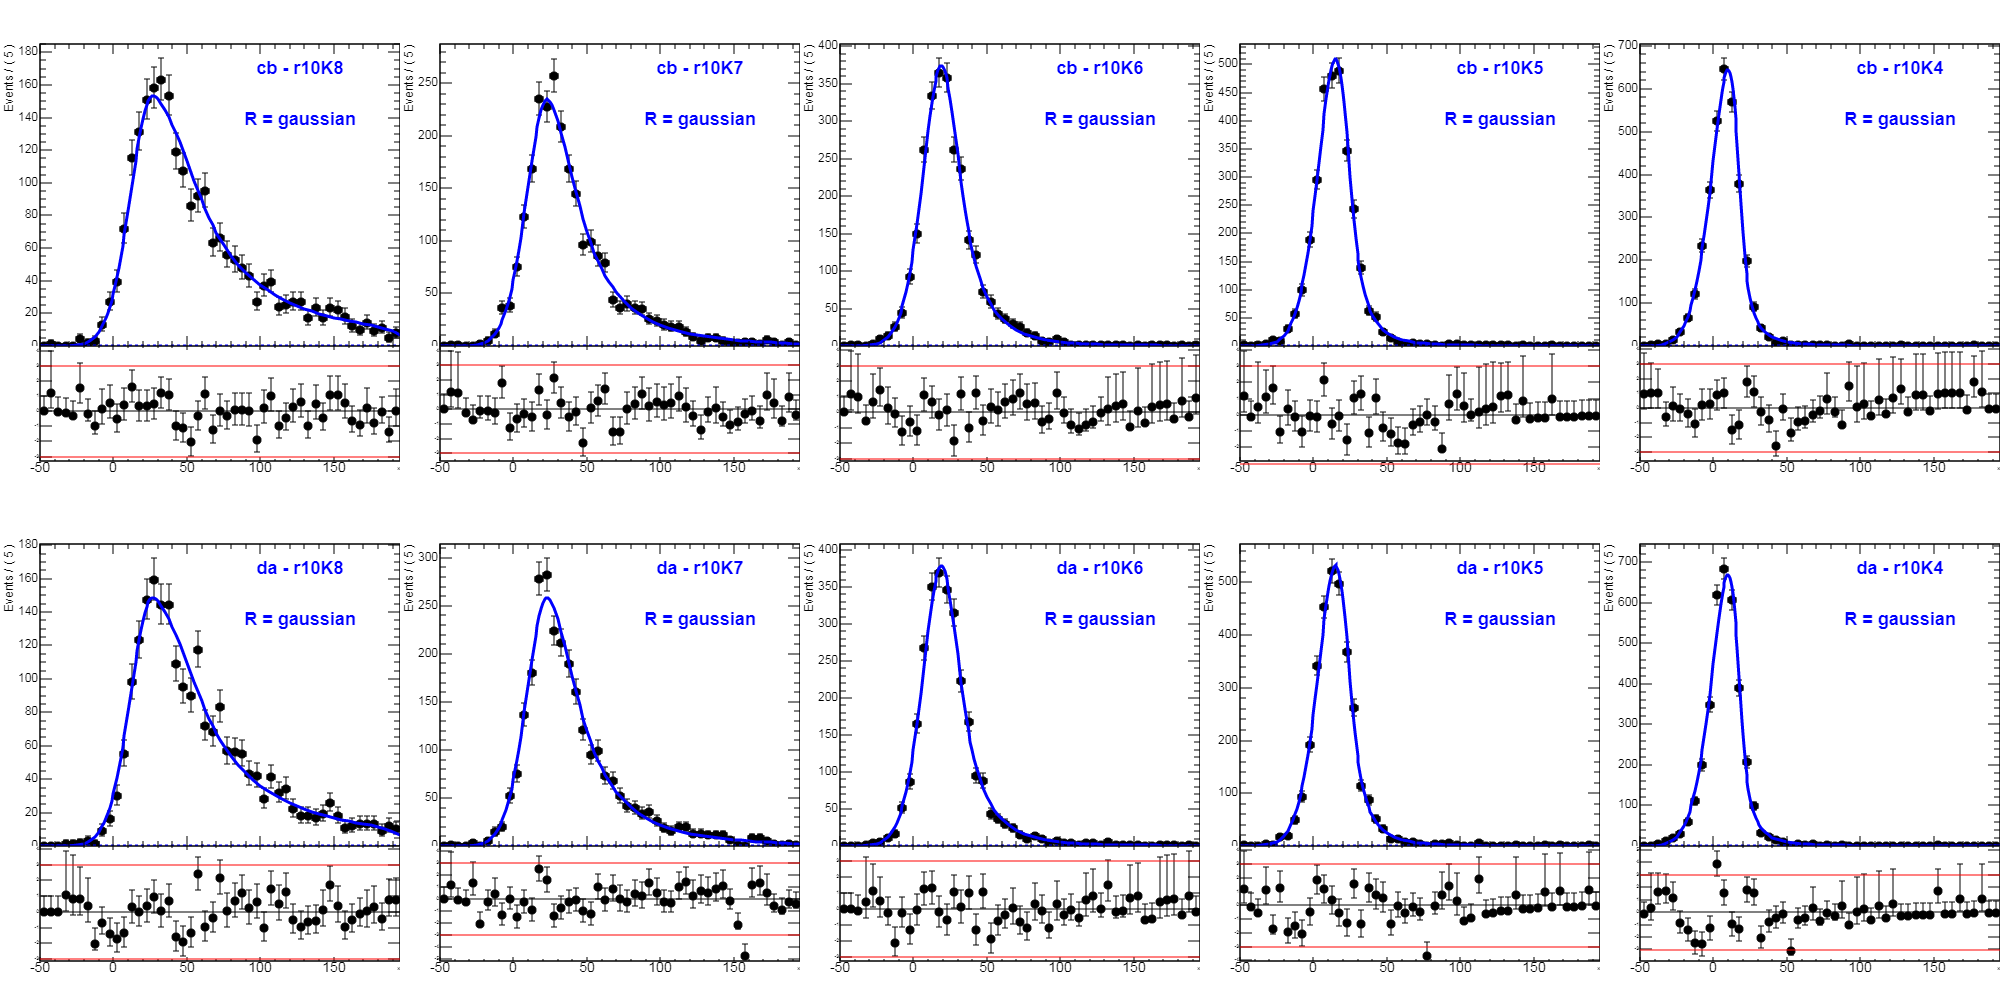
\includegraphics[width=0.65\paperwidth]{figures/chapter 4/2023_CB_gaus.png}\\
    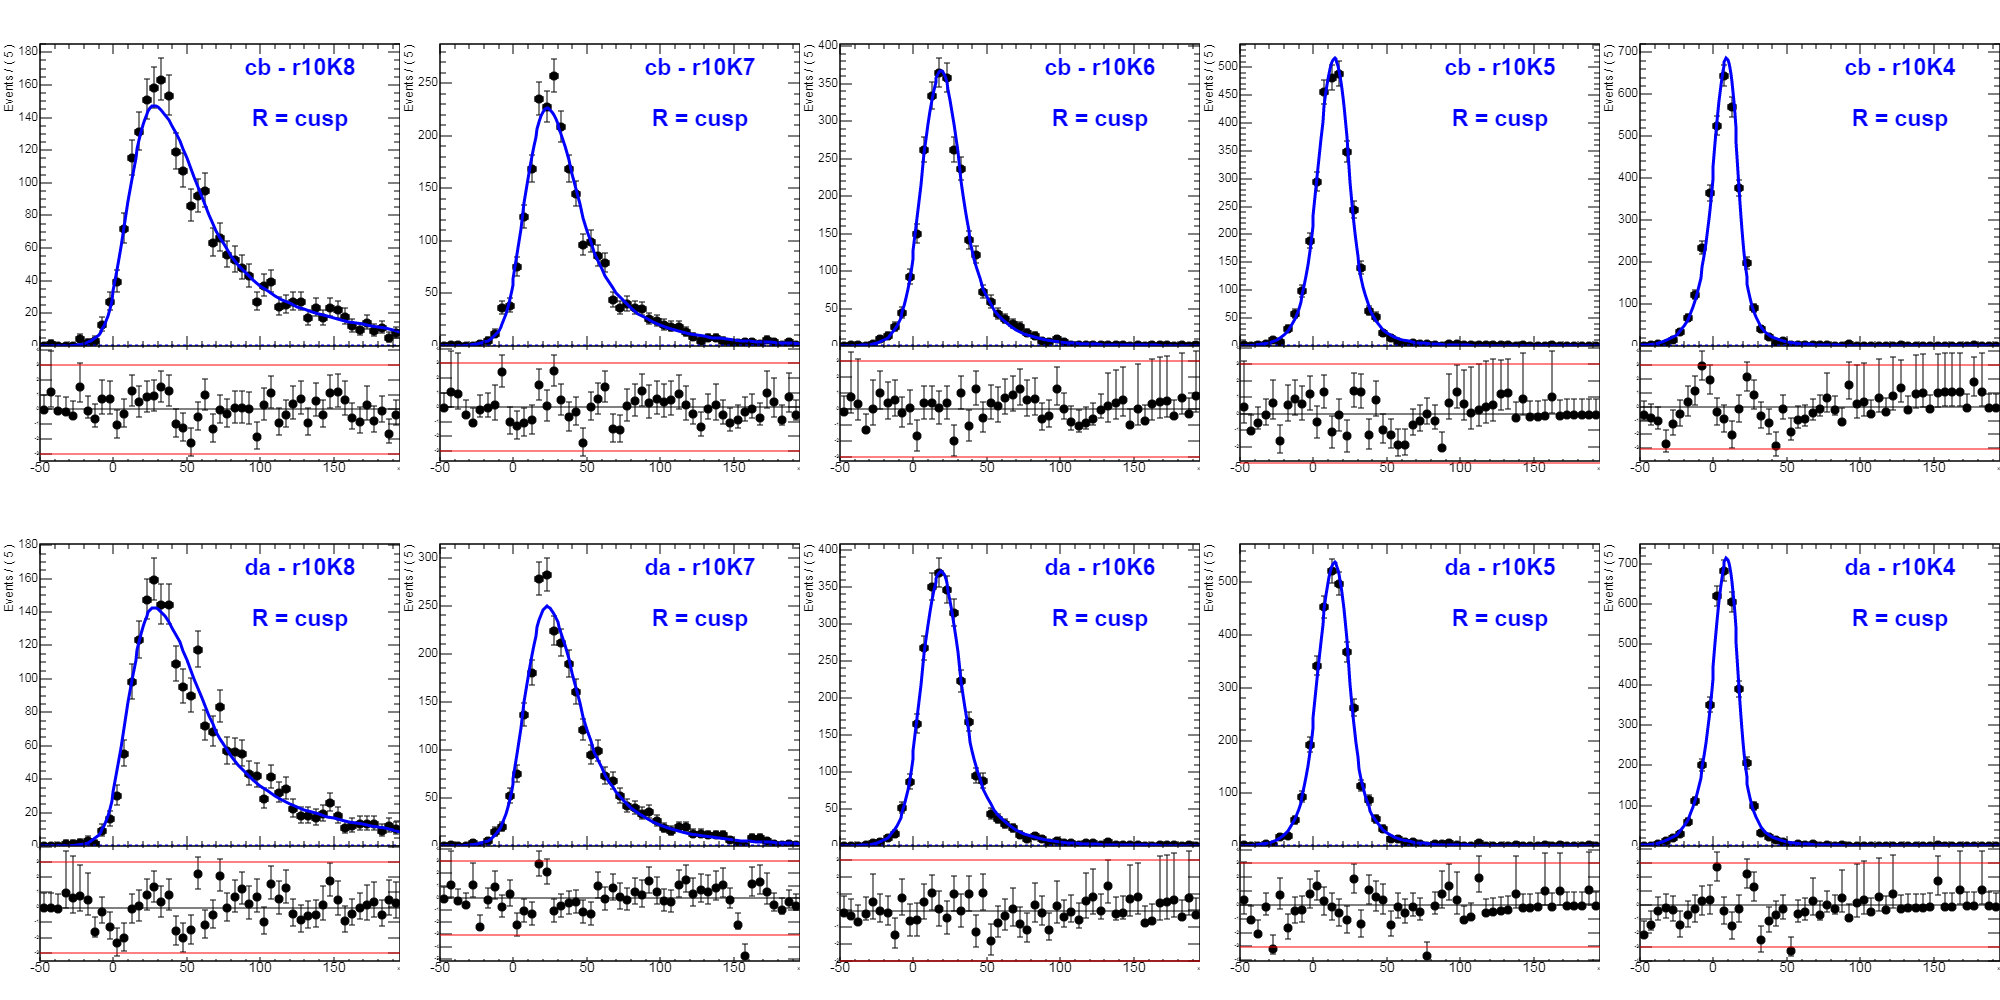
\includegraphics[width=0.65\paperwidth]{figures/chapter 4/2023_CB_cusp.png}
    \caption{Top two rows: 2023 simulations for \cb and \da transitions (the parameters are shared) with one-sided gaussian resolution function. Bottom two rows: 2023 simulations for \cb and \da transitions (the parameters are shared) with one-sided cusp function.}
    \label{fig:sim2023}
\end{sidewaysfigure}

\begin{sidewaysfigure}[hp]
    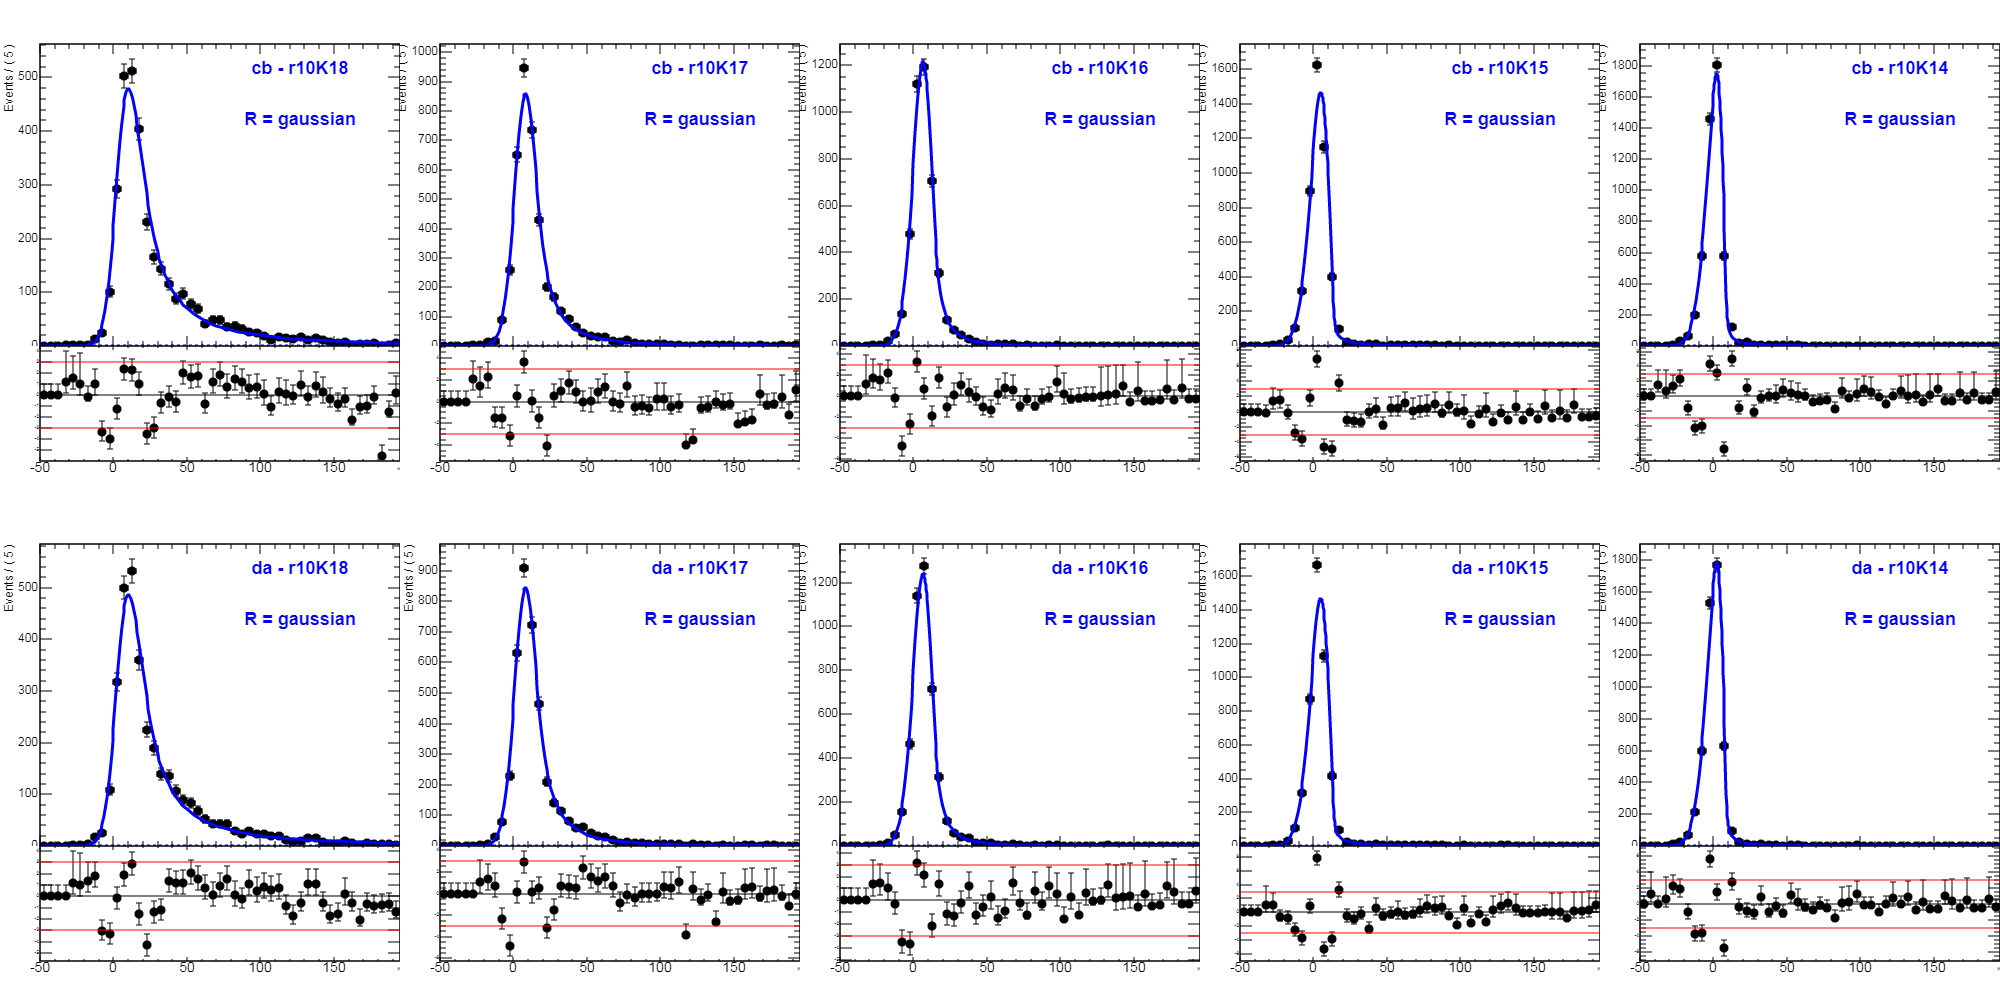
\includegraphics[width=0.65\paperwidth]{figures/chapter 4/2024_CB_gaus.png}\\
    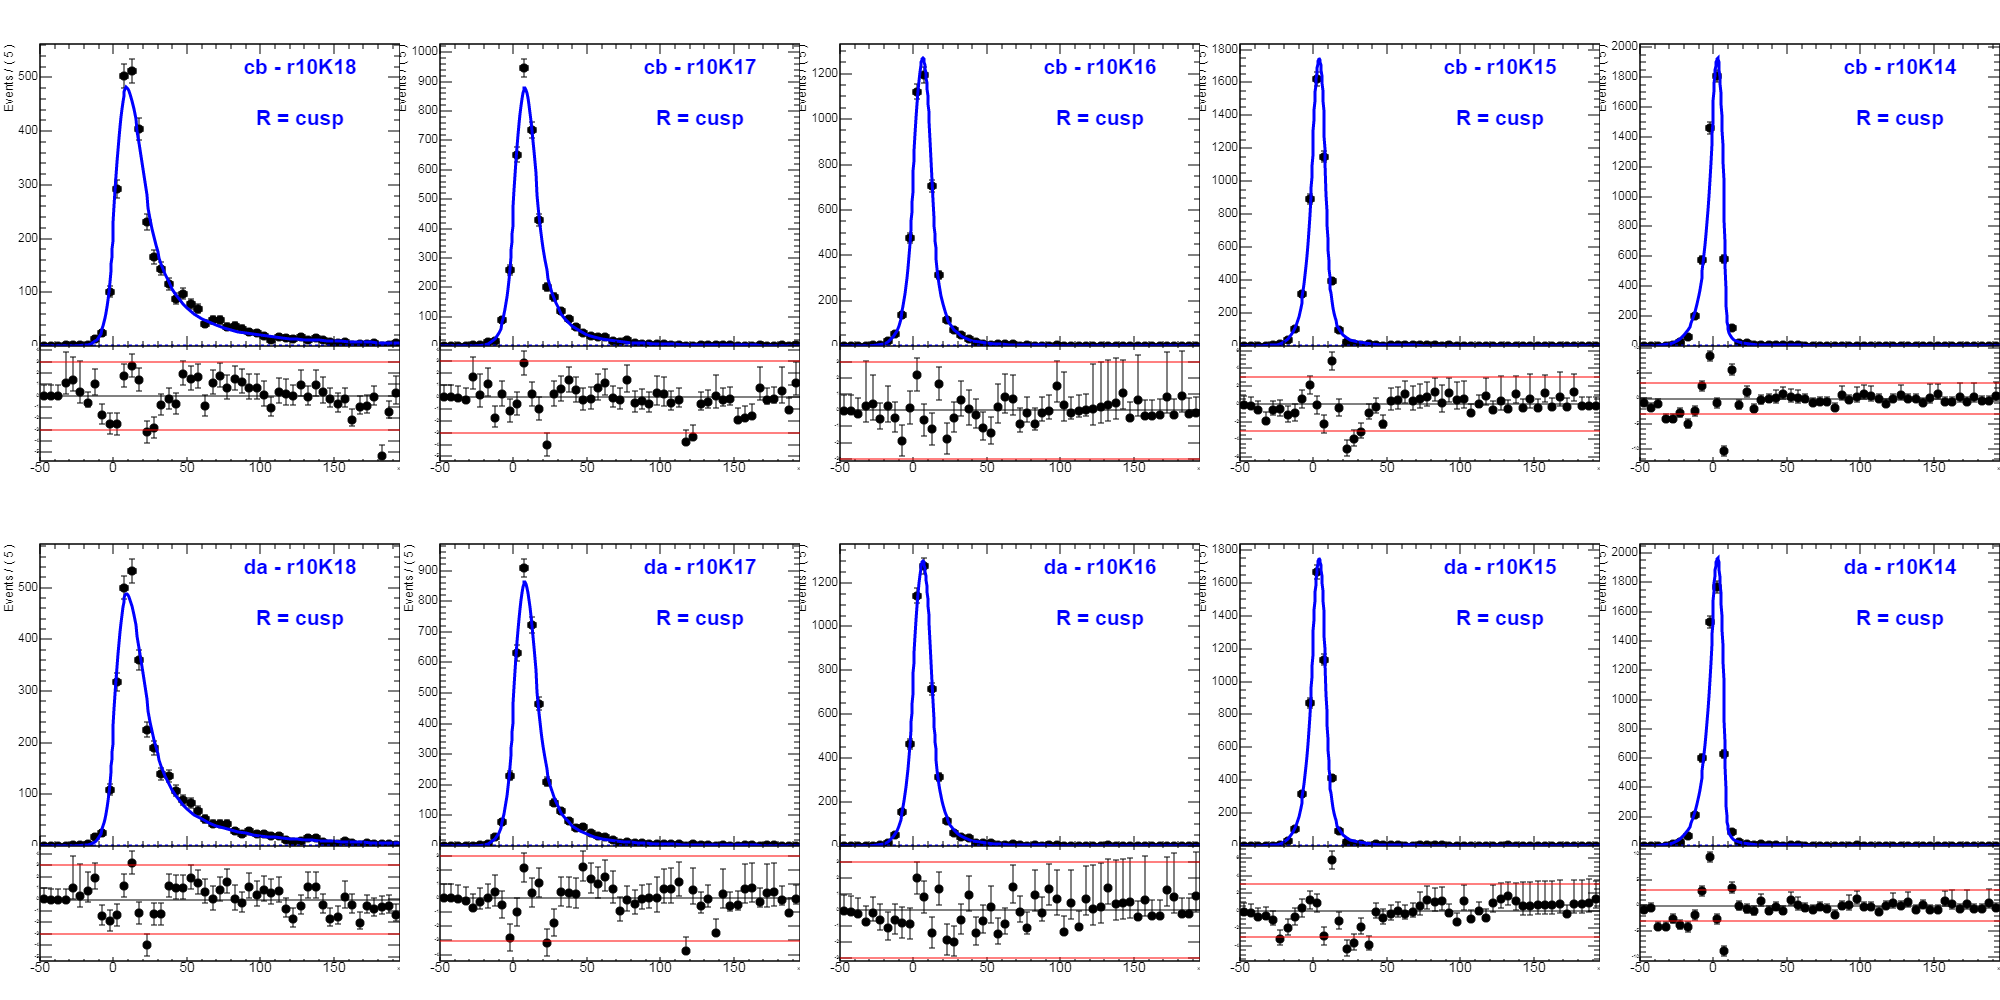
\includegraphics[width=0.65\paperwidth]{figures/chapter 4/2024_CB_cusp.png}
    \caption{Top two rows: 2024 simulations for \cb and \da transitions (the parameters are shared) with one-sided gaussian resolution function. Bottom two rows: 2024 simulations for \cb and \da transitions (the parameters are shared) with one-sided cusp function.}
    \label{fig:sim2024}
\end{sidewaysfigure}

In the nominal analysis we have used the one-sided Gaussian function as the resolution function and used the asymmetric
cusp for the model systematic. The results of the fit are summarized in Tab.~\ref{tab:resfun}. For the nominal fit to the experimental data, the broadening value was fixed to $t_{gauss} = 10 \; kHz$, as the mean value between the simulation datasets (which for simplicity are labeled as 2023 and 2024). The results indicate a reasonable range of variation of $t_{gauss}$ between the \cb and \da simulated spectra. This range of variation was used in the analysis to estimate the systematic effect related to our ignorance of the different value of broadening between the two transitions. The results are reported in Tab.~\ref{tab:results}, in the block \textit{Resolution function}: the sub-block \textit{(choice)} contains the variations of the functional form (one-sided cusp instead of one-sided Gaussian) and of the broadening common to the two transitions, while the sub-block \textit{(frequency marker)} contains mainly the variations of the broadening of one transition with respect to the other.

\begin{table}[!h]
    \centering
    \begin{tabular}{l|cc|cc}
\hline\hline
 & \multicolumn{2}{c|}{\bf Gaussian (Eq.~\ref{GaussR})} & \multicolumn{2}{c}{\bf Cusp (Eq.~\ref{CuspR})} \\ 
{\bf   Power (V/m)}  & {\bf 2023} & {\bf 2024} & {\bf 2023} & {\bf 2024}  \\
 \hline
   & \multicolumn{2}{c|}{$k$} & \multicolumn{2}{c}{$k$} \\ 
all (shared)    &  $2.47 \pm 0.2$ & $1.23 \pm 0.3$ & $1.13 \pm 0.03 $ & $0.77 \pm 0.02 $ \\
\hline  
    & \multicolumn{2}{c|}{$t_{gauss}$} & \multicolumn{2}{c}{$t_{cusp}$} \\ 
38	  & $14.8 \pm 0.2 $ & $8.9 \pm 0.1 $ & $9.1 \pm 0.2 $ & $6.3 \pm 0.1 $ \\
27	  & $14.4 \pm 0.3 $ & $8.8 \pm 0.1 $ & $8.0 \pm 0.2 $ & $5.0 \pm 0.1 $ \\
19	  & $13.9 \pm 0.3 $ & $7.7 \pm 0.1 $ & $7.2 \pm 0.2 $ & $4.6 \pm 0.1 $ \\
13.5  & $13.8 \pm 0.4 $ & $7.3 \pm 0.1 $ & $6.8 \pm 0.3 $ & $4.2 \pm 0.1 $ \\
9.5	  & $13.6 \pm 0.6 $ & $7.0 \pm 0.2 $ & $6.4 \pm 0.4 $ & $3.8 \pm 0.1 $ \\
     \hline \hline
 \end{tabular}
    \caption{Results of the fit to simulations in terms of $t_{gauss}$ for a Gaussian resolution function (see Eq.~\ref{GaussR}) and of $\tau$ for a Cusp resolution function (Eq.~\ref{CuspR}).}
    \label{tab:resfun}
\end{table}

\subsubsection{Doppler broadening} \label{sec:Doppler}

The simulations described in Sec.~\ref{sec:Simulation} do not include the Doppler effect, whose contribution to the broadening must therefore be estimated separately. Assuming a Maxwell-Boltzmann distribution for the energy of the trapped anti-atoms, and that only the component of the velocity along the direction of propagation of the microwave radiation contributes to the shift, the corresponding velocity ratio $\beta_z = v_z / c$ is normally distributed with standard deviation

\begin{equation}
\beta_z = \sqrt{\frac{k_B T}{m_{\overline{H}} c^{2}}} \, .
\end{equation}

For non-relativistic velocities the Doppler shift is $\Delta f = f - f_o = - |\beta_z| f_o$, where $f_o$ is the frequency delivered by the synthesizer. The absolute value accounts for the fact that the frequency scan is always performed from below, so that the resulting contribution to the resolution function is again one-sided, with width

\begin{equation}
\sigma_{Doppler} = \sqrt{\frac{k_B T}{m_{\overline{H}} c^{2}}} \; f_o \, .
\end{equation}

For $f_o \simeq \SI{30}{\giga \hertz}$ and an anti-atom energy distribution with a mean of $T \simeq \SI{0.36}{\kelvin}$, as measured in \cite{ALPHA:2024adiab}, this gives $\sigma_{Doppler} \simeq \SI{5}{\kilo \hertz}$; taking instead the full trap depth $T = \SI{0.5}{\kelvin}$, which is a conservative upper limit for the energy of the trapped sample, yields $\sigma_{Doppler} \simeq \SI{6}{\kilo \hertz}$.

These values are smaller than, but of the same order as, the broadening $t_{gauss} = \SI{10}{\kilo \hertz}$ extracted from the simulations and used in the nominal fit. It is therefore worth stressing that this contribution is already covered by the systematic uncertainty assigned to the resolution function: adding it in quadrature to the simulation-derived value would give an effective width of \SI{11}{\kilo \hertz} to \SI{12}{\kilo \hertz}, which lies well inside the interval $t_{gauss} \in [7.0, 13.6]\,{\rm kHz}$ explored in Tab.~\ref{tab:results}, where the induced shift of the hyperfine splitting never exceeds \SI{1.1}{\kilo \hertz}. Moreover, the estimate above should be regarded as an upper bound, since it treats each anti-atom as if it sampled the microwave field with a fixed longitudinal velocity, whereas the field in the trap is a standing wave and each atom traverses it many times within a single \SI{8}{\second} frequency step, so that the first-order Doppler contribution is largely averaged out. \commento{riassumere qui in una frase l'argomento dell'elog ALPHA/33017}

%\newpage

\subsection{Reproducibility: shape variation during the experiment} \label{sec:Reproducibility}

A possible systematic uncertainty is linked with the assumption that the shape of the spectra does not change from repetition to repetition. This assumption is used implicitly in the fit protocol, since the parameters controlling the shape of the signal model ($\sigma$, $\sigma_{r}$, and $n_{r}$) are constrained to be the same for all the \cb and \da repetitions, respectively. Hence, a dedicated study is necessary to evaluate this uncertainty.

The variation of the shape of the spectra is something expected during the measurement. There are a number of physical arguments that indicate this. At first, the energy distribution of the atom ensemble produced during the experiment can vary from repetition to repetition (although the anti-atoms are accumulated along 20 mixing cycles, and the final energy fluctuation is expected to be averaged over 20 cycles). More importantly, since the current of the main solenoid is drifting and decreasing over time, the microwave frequency must be adjusted to follow the magnetic field drift. Hence, the working point of the frequency scan changes from repetition to repetition. Following that, the microwave standing wave pattern can change, as well as the effective power delivered to the trap. Additionally, although the magnetic field profile could change during the measurement, both its on-axis profile (which can be monitored by ECR measurement) and its off-axis profile (which is unmonitored) can fluctuate due to current fluctuations in the magnets. The magnetic field profile is monitored using direct-current current transformers based on magnetometer sensors (ITZ 2000-SB FLEX ULTRASTAB from LEM International SA), and its value is used as input to PIDs that ensure the stability of each individual magnet (more details in Sec.~\ref{sec:DCCTs}).

Shape variations are expected to have a non-negligible impact on the measurement. As mentioned before, the correlation between the shape parameters and the frequency markers is strong (see Fig.~\ref{fig:CorrelationHeatMap}). Hence, shape variations from repetition to repetition are expected to consistently change the extracted value. For this reason, the experimental protocol incorporated high-statistics reference measurements, which were used to estimate the magnitude of these variations. The high-statistics sample measurement has a statistical power 5-6 times that of a single repetition. These data have been fitted independently, with the same model used in the nominal Maximum Likelihood Fit, and the results are shown in Fig.~\ref{fig:FitTOHighStats}. The parameters resulting from the fit are reported in Tab.~\ref{tab:highstatparam}.


\begin{sidewaysfigure}[hp]
\centering
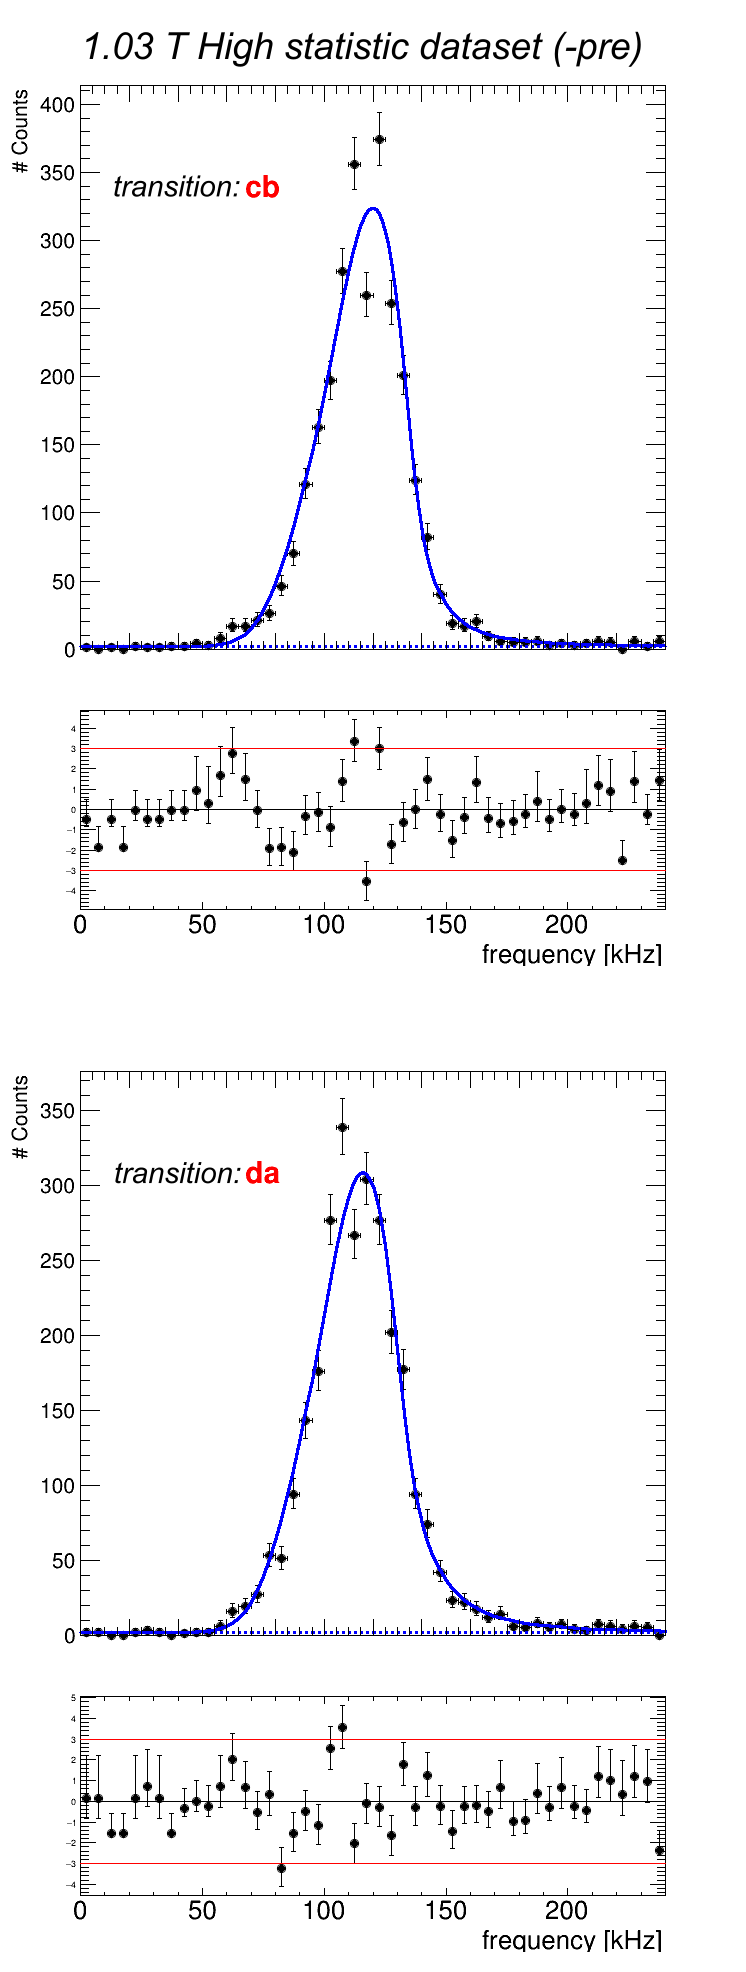
\includegraphics[width=5.2cm]{figures/chapter 4/s8_pre_v.png}  %
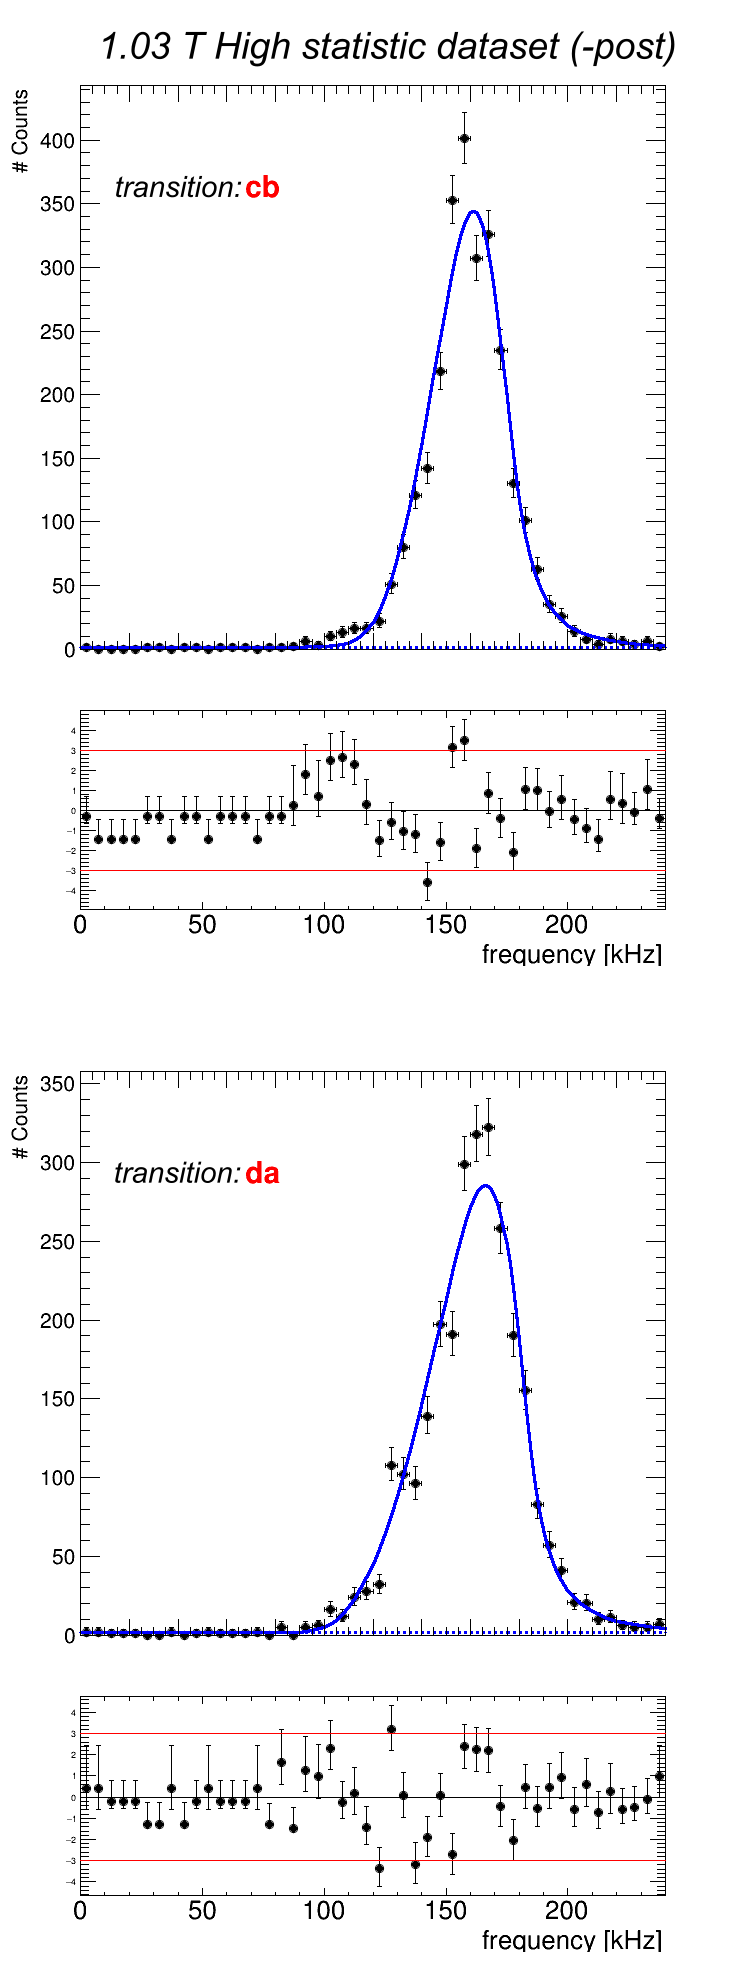
\includegraphics[width=5.2cm]{figures/chapter 4/s8_post_v.png} %
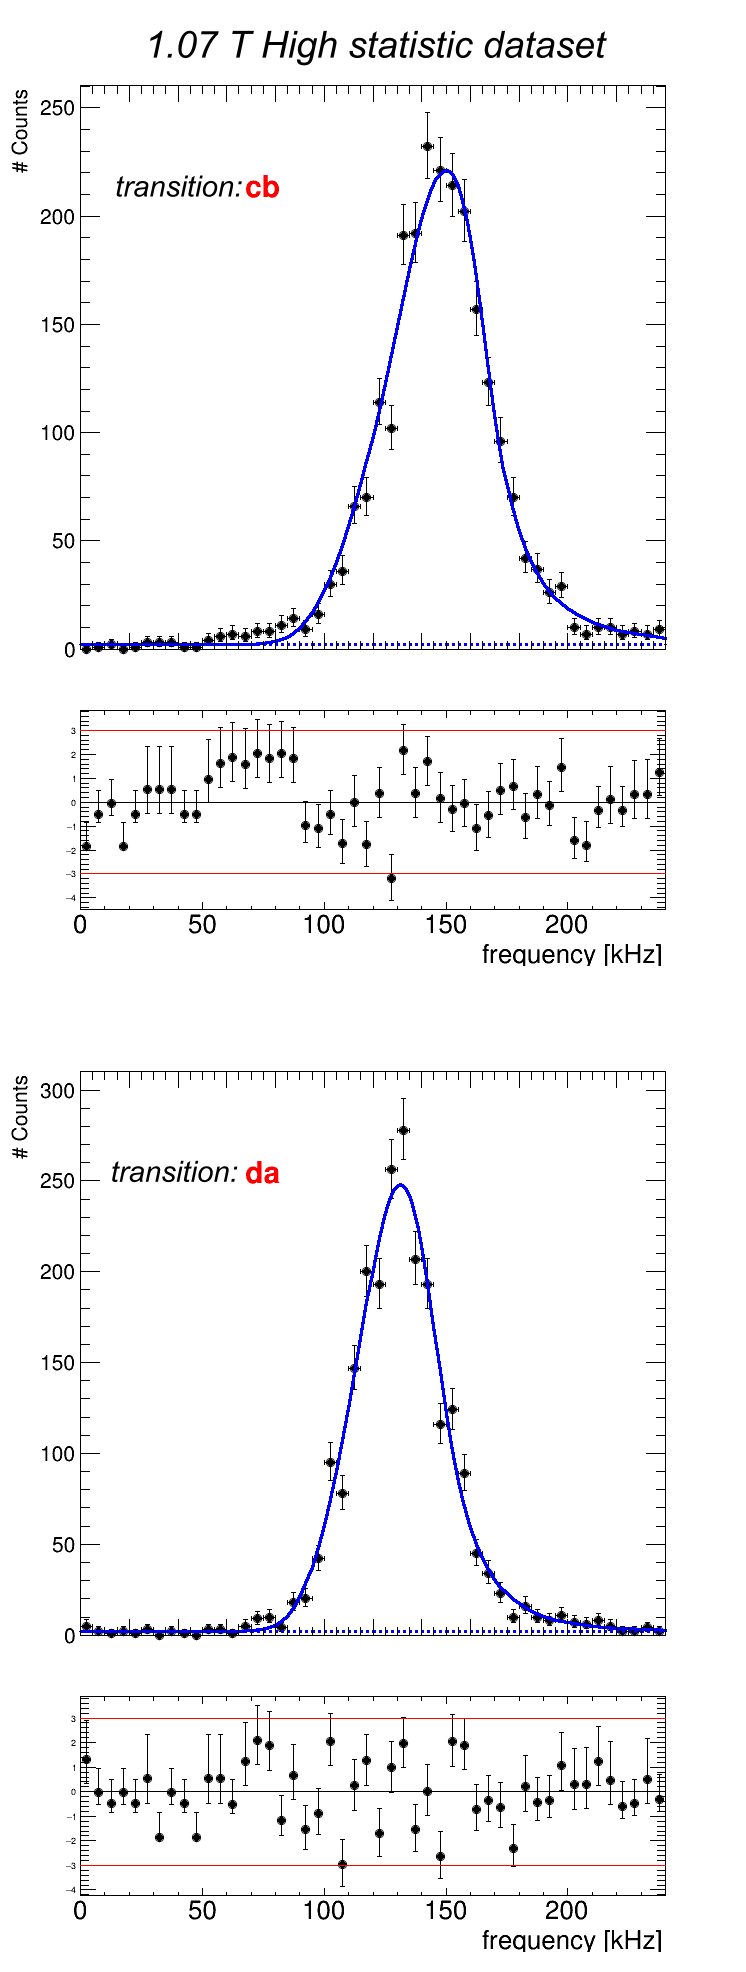
\includegraphics[width=5.2cm]{figures/chapter 4/s7_post_v.png} %
\caption{High statistic dataset for the two magnetic field configuration of the experiment. The \textit{-post} label indicated that the dataset has been acquired after the nominal 8 repetitions, the \textit{-pre} indicated that the dataset has been acquired before the nominal 8 repetitions. The fit function (blue continuous line) is the best fit result with the same model of Eq.~\ref{eq:model1}. This model constitutes a ``template'' used to estimate reproducibility uncertainty.}
\label{fig:FitTOHighStats}
\end{sidewaysfigure}

\begin{table}[!h]
\centering
\resizebox{\columnwidth}{!}{
\begin{tabular}{l|ccc}
\hline
\hline
\textbf{}  & \textbf{\SI{1.07}{\tesla} post}   & \textbf{\SI{1.03}{\tesla} pre}  &  \textbf{\SI{1.03}{\tesla} post}  \\
\hline 
$n^{(cb)}$                &  $4.3 \pm 1.7 $     & $5.1 \pm 0.9$   & $6.4 \pm 2.9$  \\
$n^{(da)}$                &  $9.8 \pm 5.6$     & $3.5 \pm 0.9$   & $3.6 \pm 1.21$  \\
$\sigma^{(cb)}_{r}$ (kHz) & $13.48 \pm  1.4$             & $7.3 \pm 0.8$   & $8.3 \pm 0.8$  \\
$\sigma^{(da)}_{r}$ (kHz) & $13.00 \pm  1.2$             & $9.0 \pm 1.0$   & $7.7 \pm 1.1$  \\
$\sigma^{(cb)}$ (kHz)     & $22.0 \pm  1.1$             & $20.3 \pm 1.0$ & $17.2 \pm 0.7$ \\
$\sigma^{(da)}$ (kHz)     & $17.1 \pm 0.9$              & $20.03 \pm 0.8$ & $24.8 \pm 0.8$ \\
$n_B^{(cb)}$              & 186 $\pm$ 25                 & 130 $\pm$ 26    &  81 $\pm$ 15   \\
$n_B^{(da)}$              & 125 $\pm$ 20                 & 86 $\pm$ 22     &  70 $\pm$ 14   \\
$n_S^{(cb)}$              & 2235 $\pm$ 51               & 2666 $\pm$ 56   &  2658 $\pm$ 53 \\
$n_S^{(da)}$              & 2175 $\pm$ 49               & 2722 $\pm$ 55   &  2716 $\pm$ 53 \\
\hline
$\Delta f$ (kHz)          & $-9.17 \pm 2.8$  &  $-8.7 \pm 2.2$  & $-20.0 \pm 2.1$ \\ %% THESE SHOULD STAY HERE. people will ask for them anyways. 
$rise^{cb}$ (kHz)         & $ 66 \pm 3$ & $ 60.8 \pm 2$ & $ 52 \pm 2$  \\
$rise^{da}$ (kHz)         & $ 51 \pm 3$ & $ 60.1 \pm 3$  & $ 74 \pm 2$  \\
\hline\hline
time from center of associated series (h) & $11.5$ & $-7$ & $11.2$ \\
duration of associated series (h) & $12$ & $11.75$ & $11.75$\\
\hline
\hline
\end{tabular}
}
\caption{Model float parameters from high statistics sample. The $\Delta f$ value (not corrected for the $B-$field drift, and blind) is shown as a cross-check.}
\label{tab:highstatparam}
\end{table}

These results can be used to evaluate the effect of shape variations on the inferred value of the hyperfine splitting. To estimate such uncertainty, only the high statistic dataset acquired after the main eight repetitions (for simplicity indicated as {\it post} distributions) have been used. Assuming a difference in shape in time, the 8 repetitions have been fitted with the model obtained from the high-statistics template, keeping all the shape parameters fixed, except the frequency markers. The full analysis procedure has been repeated and the hyperfine splitting obtained with this alternative approach has been compared with the nominal one to evaluate the systematic uncertainty. 
Since the {\it post} data were collected about $\Delta t_{post} = 12$ hours after the middle of the Physics {\it Series}, which lasted about $T_{series} = 12$ hours (see Tab.~\ref{tab:ListOfRuns}), the difference in the result has been divided by 2 (considering that the Series extends $\pm T_{series}/2 \approx \pm \Delta t_{post}/2$ around the center of the Series). This estimate resulted in \SI{2.8}{\kilo\hertz} for the high-field series (\SI{1.07}{\tesla}), \SI{7.0}{\kilo\hertz} for the low-field series (\SI{1.03}{\tesla}) and \SI{2.7}{\kilo\hertz} for their combination. The best-fit parameters for the high-statistics sample are reported in Tab.~\ref{tab:highstatparam}, while the resulting shifts of the hyperfine splitting are reported in Tab.~\ref{tab:results}, in the block \textit{Lineshape reproducibility}.

Another cross-check has been performed comparing the result of the hyperfine splitting measurement, once imposing a common rise (parameter $r$ in Eq.~\ref{eq:model1}) for the 8 repetitions (the way it is done for the measurement) and once leaving such parameter to vary across the 8 repetitions (see Fig.~\ref{fig:free_rise}) as described in Sec.~\ref{checks}. 



\subsection{Data Selection and Binning}

Uncertainties can be introduced due to the time of flight of the anti-hydrogen before annihilation and to some synchronization uncertainties. An estimate of this systematics has been evaluated by subtracting $30\,{\rm ms}$ from the time of the event, before associating the time to the frequency step. The difference with respect to the nominal case is found to be negligible. 

Binning is also a source of systematic uncertainties. All the $cb$ and $da$ scans are in fact separated by a fixed frequency difference $\delta f_{window} = 1\,420\,390\,{\rm kHz}$, which is a multiple of the $\delta_{bin} = 5\,{\rm kHz}$ frequency step. The binning chosen for the nominal analysis is aligned to the frequency step for both transitions, and the starts of the two histograms are separated by  $\delta f_{window}$. Due to the discrete nature of the scan, different choices of the binning start would have resulted in the same histograms, e.g., by starting the binning of any transition up to $\delta_{bin} -\varepsilon$ later ($\varepsilon$ is an arbitrarily small number). We assign a systematic uncertainty of $\frac{\sqrt{2}\delta_{bin}}{\sqrt{12}} = 2.0\,{\rm kHz}$ to account for this degeneracy. Both results are reported in Tab.~\ref{tab:results}, in the block \textit{Data selection and binning}.


\subsection{Short Term Upward Drift} \label{sec:ShortDrift}

The long-term linear drift is not the only effect requiring careful treatment. A short-term upward drift may also occur during the experiment. This is expected because the accumulation and stacking phase between repetitions involves changes to the beam-line magnets. Although the main solenoid magnets and mirror coil currents are not changed during this operation, the beam-line magnets must be changed, for the plasma manipulation and transport from the catching region to the atom trap. Parasitic currents could be induced in the solenoid through mutual coupling, producing a magnetic field shift distinct from the linear drift. Since the experiment is based on a \cb transition followed by a \da transition, an induced shift in the magnetic field is directly related to a systematic shift of all the \da transitions due to the Zeeman effect. Hence, a systematic shift in the splitting of the transition is expected, which is unrelated to the physical splitting.

In principle, this effect can be estimated through theoretical calculation of the parasitic currents induced from the beam-line magnets to the mirror coils and the superconducting solenoid. In practice, this approach is challenging, given the required target accuracy of this measurement. So a data driven approach was followed.

The systematic uncertainty associated with this effect has been constrained using data taken in 2023, following an experimental protocol similar to the one used for the 2024 campaign, but with specific modifications to isolate and study this effect. The protocol consisted of repeating the same measurement, a \cb and \da transition pair, with a deliberate delay introduced in the sequence between the final manipulation of the beam-line currents and the start of spectroscopy. In the first variant, the spectroscopy began \SI{32}{\second} after the last manipulation of the beam-line magnet change. In the second variant, the delay was set to \SI{352}{\second}. The delays were chosen in such a way that the \cb measurement with the second protocol coincides in time with the \da measurement of protocol 1, and the data taking consisted of alternately repeating one measurement with protocol 1 and one with protocol 2. Apart from this modification, the data-taking procedure was analogous to that employed in 2024. 6 repetitions with the first protocol and 5 repetitions with the second were taken, to correct the linear magnetic field drift and extract the transition splitting. In the following analysis, we denote $cb_{32s (352s)} ; da_{32s (352s)} $ as the frequency marker intercepts from the linear fit corresponding to the first (second) protocol. The frequency shifts induced by the short-term upward magnetic drift can then be expressed as follows:

\begin{align*}
\Delta _{cb} &= cb_{32s}  - cb_{352s} \\
\Delta _{da} &= da_{352s} - da_{32s}
\end{align*}

Three combinations of splitting can be determined from the analysis of the experimental data. The spectra were fitted using the same lineshape function as in the 2024 analysis, and the fit to the frequency markers has been performed with a slope constrained to be common to all four lines (see Fig.~\ref{fig:ShortUpwardBdrift}). Because the \cb for protocol 2 and \da for protocol 1 occur at the same time relative to the last magnet manipulation, it follows that:


\begin{figure}[!htbp]
\centering
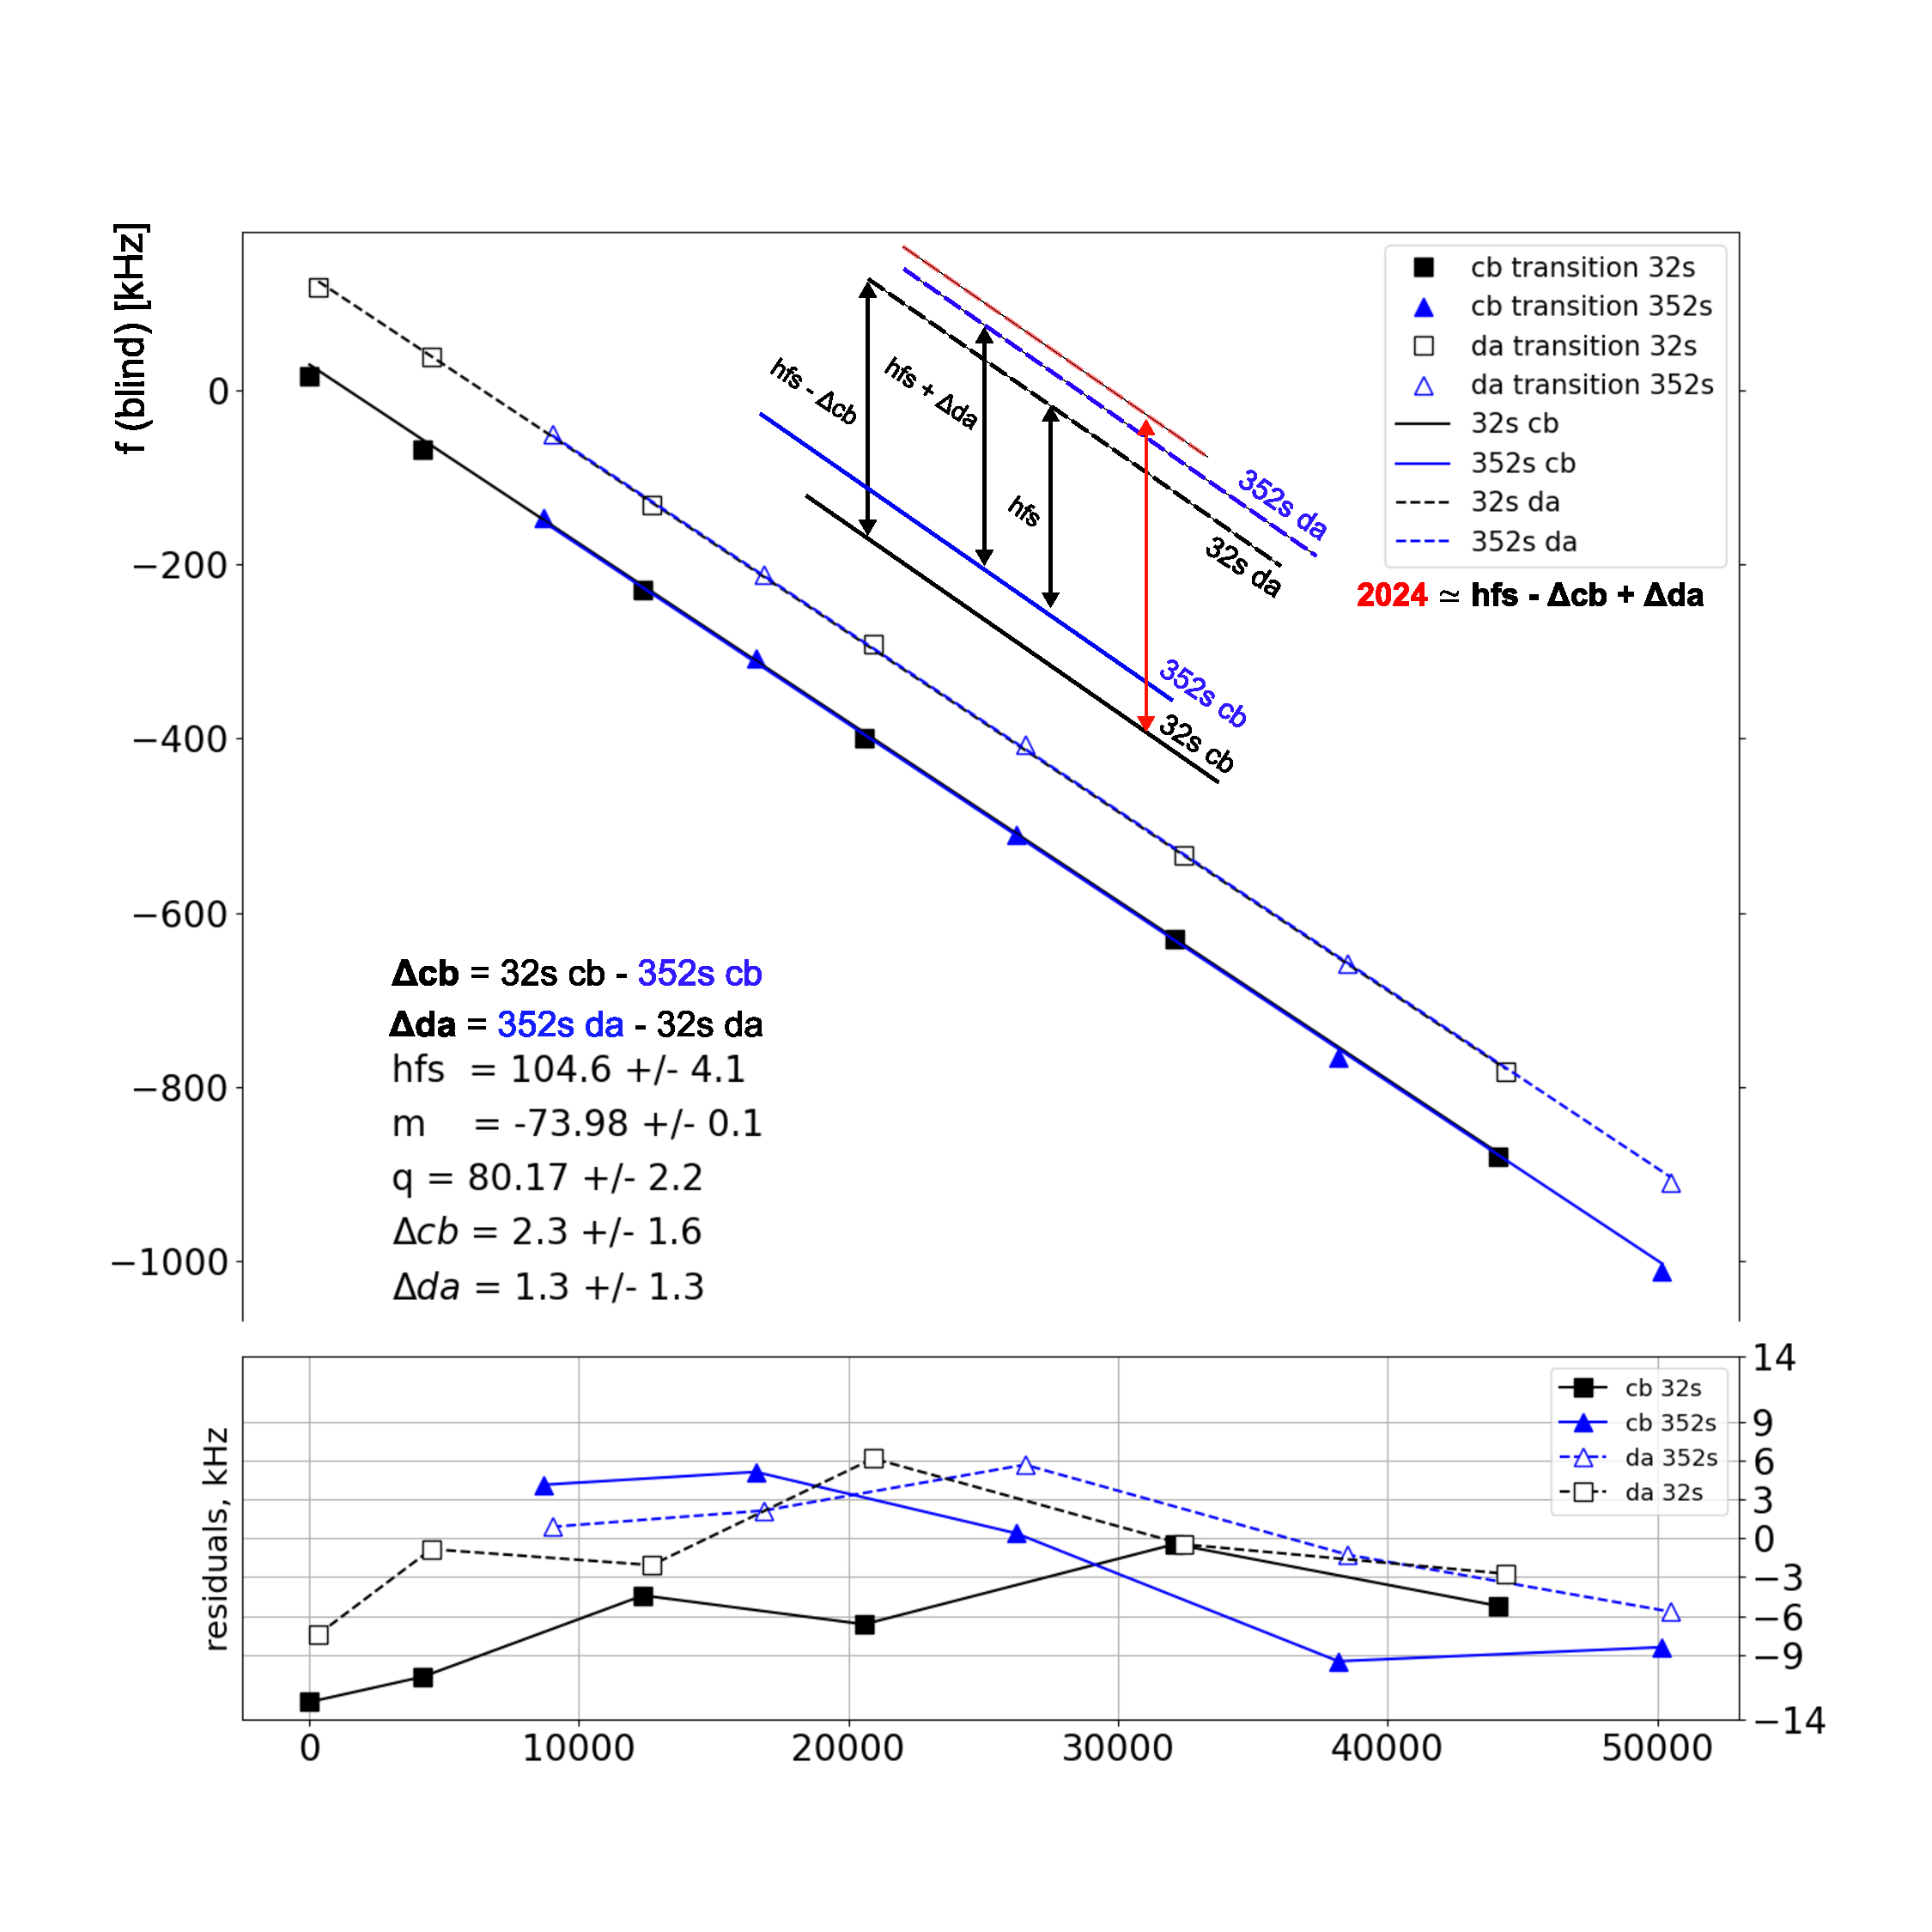
\includegraphics[width = \textwidth]{figures/chapter 4/upwardshort.pdf}
\caption{This plot shows the results from the analysis of the 2023 data. This analysis has been used to constrain magnetic upward drift induced from beam-line magnet manipulation during antihydrogen stacking phase. The change of the beam-line magnets during stacking can induce parasitic currents on Mirror and Solenoid magnets, causing a small magnetic upward drift. Since the \da transition always follows the \cb transition, this effect can generate a systematic shift in the frequency that changes the value of the splitting. This shift has been constrained using 2023 data that were collected with two protocols. In the first protocol there are \SI{32}{\second} between the last manipulation of the beam-line magnets and the start of the microwave measurement. In the second protocol the time interval is increased to \SI{352}{\second}. With this setup, the \cb transition with the \SI{352}{\second} delay starts at the same time, with respect to the beam-line magnet manipulation, of the \da transition with the \SI{32}{\second} delay. The frequency markers shown are the result of the analysis on Pass Cuts data.}
\label{fig:ShortUpwardBdrift}
\end{figure}


\begin{equation*}
a_{1S}/h = da_{32s} - cb_{352s}
\end{equation*}

The other two quantities of interest are:

\begin{align*}
da_{352s} - cb_{352s} &= da_{32s} + \Delta_{da} - cb_{352s} = a_{1S}/h + \Delta_{da}  \\
da_{32s}  - cb_{32s}  &= da_{32s} - \Delta_{cb} - cb_{352s} = a_{1S}/h - \Delta_{cb}
\end{align*}

The linear fit was performed with the same minimization technique (extended least-square), with a common slope $m$, the hyperfine splitting $a_{1S}/h$, common offset $q$ and shifts $\Delta_{cb}$ and $\Delta_{da}$ as free parameters. The best fit values have been reported in Fig.~\ref{fig:ShortUpwardBdrift}. 
The 2024 data taking had the \cb measurement starting \SI{32}{\second} after the beam-line manipulation, and the \da transition was measured after \SI{512}{\second} + \SI{300}{\second} of wait. So the overall shift can be approximated as:

\begin{equation}
da_{2024} - cb_{2024} \simeq da_{352s} - cb_{32s} = a_{1S}/h - \Delta_{cb} + \Delta_{da}
\end{equation}

From this analysis, the systematic shift due to the short-term upward magnetic shift was estimated as $\sigma_{shift} = |  \Delta_{da} - \Delta_{cb}| = 1 \; kHz$. This value has been added in quadrature as a systematic uncertainty to the overall error budget of the measurement, and is reported in Tab.~\ref{tab:results}, in the block \textit{B-drift (short time scale drift)}.


\subsection{Magnetic decay over time} \label{sec:decaySystematic}

As mentioned in the experimental protocol (Sec.~\ref{Protocol-of-experiment}), the decay of the magnetic field has to be corrected in the analysis to extract the hyperfine splitting. The magnetic field drift can be characterized with ECR measurement and with spectroscopy itself. In the current analysis, no ECR measurements were used to account for the drift, and the magnetic field has been introduced as a parameter in the common linear fit. Hence, an assumption of a linear decay has been used in the main analysis, and a systematic uncertainty must be assigned to account for this particular choice.

A first alternative is the so-called ``split'' method, which was used in a previous version of the analysis and provides an estimate of the hyperfine splitting for each individual repetition. Instead of the common fit, two separate linear fits are performed to the \cb and to the \da frequency markers, and the average of the two slopes, $m_{split} = (m_{cb} + m_{da})/2$, is used to correct the difference between the two markers of each repetition for the field drift that occurs during the interval $\Delta t = \SI{812.4}{\second}$ between the two scans:

\begin{equation}
\Delta f^{(i)}_{corr} = f_{da}^{(i)}(t_i + \Delta t) - m_{split} \Delta t - f_{cb}^{(i)}(t_i) \, .
\end{equation}

With slopes between about $-72$ and \SI{-76}{\kilo\hertz\per\hour}, the correction amounts to roughly \SI{17}{\kilo\hertz}. The hyperfine splitting is then obtained from the average of the eight $\Delta f^{(i)}_{corr}$ of each series, to which the separation $\delta f_{window}$ between the two scans is added. The results of the ``split'' method differ from the nominal ones by \SI{-2.3}{\kilo\hertz} and \SI{+0.5}{\kilo\hertz} for the high-field and low-field series, respectively, as reported in Tab.~\ref{tab:results}, in the block \textit{B-drift (fit procedure)}. The origin of this discrepancy has been attributed to the fact that the ``split'' method neglects the off-diagonal blocks of the covariance matrix of Tab.~\ref{tab:cov_matrix}, i.e.\ the correlation between the differences $\Delta f^{(i)}$ and the \cb markers, which is instead taken into account by the common GLS fit.

A Gaussian process regression (\textit{GPR}) technique has been employed as a second alternative method to correct for the magnetic field drift over time. Instead of testing different decay models, Gaussian process regression uses non-parametric supervised learning methods to solve regression problems. This method allows for an alternative estimate of the hyperfine splitting without relying on the assumption of a linear decay of the field. This technique has been applied to the average of the frequency markers:

\begin{equation}
\overline{f}^{i} = \dfrac{f^{i}_{cb} + f^{i}_{da}}{2}
\end{equation}

 The $\Delta_{f}^{i} = f_{da}^{i} - f_{cb}^{i}$ have been corrected for the magnetic field drift individually (by estimating the frequency shift from the time interval between the \cb and \da, i.e.\ \SI{812.4}{\second}, and considering each individual local magnetic drift). The result of the GPR interpolation is shown in Fig.~\ref{fig:GPR}.

\begin{figure}[!htbp]
    \centering
    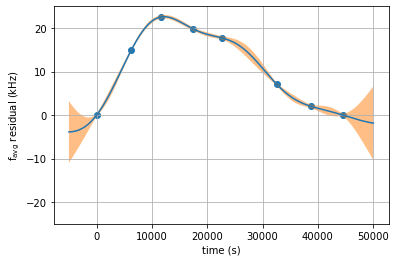
\includegraphics[width=0.49\linewidth]{figures/chapter 4/s7_residual_gpr0.2.png} 
    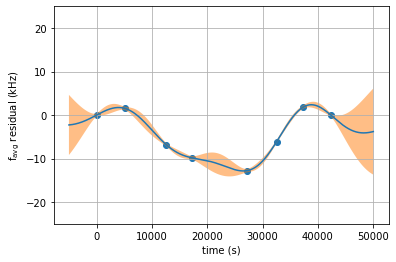
\includegraphics[width=0.49\linewidth]{figures/chapter 4/s8_residual_gpr0.2.png} \\
    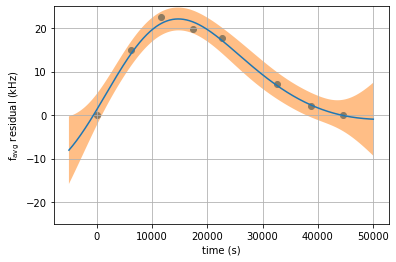
\includegraphics[width=0.49\linewidth]{figures/chapter 4/s7_residual_gpr2.0.png} 
    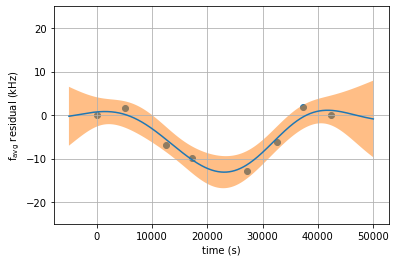
\includegraphics[width=0.49\linewidth]{figures/chapter 4/s8_residual_gpr2.0.png} 
    \caption{Interpolation of the $cb$ frequency markers (points) with Gaussian Process Regression for the high-field (left) and low-field (right) series. The linear trend is removed before interpolation 
    (detrending is such that the ordinates of the first and last points are zero). The abscissa is the time of the repetition in seconds and the ordinate is the residual w.r.t. the linear trend of the frequency markers, in kHz. The band represents the $95\%$ confidence interval.
    Top and bottom figures are obtained with different settings for the input noise, without significant changes in the estimate of the systematic uncertainty. The top plots correspond to the settings used for the estimate in Tab.~\ref{tab:syst}.}
    \label{fig:GPR}
\end{figure}

Since the GPR correction is applied to the individual differences, the result is compared with the ``split'' method with linear correction. The differences between the two are \SI{-0.3}{ \kilo \hertz} and \SI{-0.1}{\kilo \hertz} for the high B-field and low B-field series, as reported in Tab.~\ref{tab:results}, in the block \textit{B-drift (long time scale linearity)}.

\subsection{DCCT Traces and Magnetic Field Fluctuation} \label{sec:DCCTs}

The magnets employed to design the microwave flat magnetic field for the measurement are supplied with hundreds of amperes, and are handled and monitored with direct-current current transformers based on closed-loop fluxgate magnetometer sensors (DCCT). The current flowing in each magnet is constantly measured by an analog-to-digital converter (NI-9239 cRIO) that digitizes the DCCT signal output, and it is used in PID control of the magnet power supply for stabilization within a few mA. In the context of the analysis, the DCCTs current traces have been analyzed to verify how stable the currents are versus time. 

\begin{figure}[hbtp]
\centering
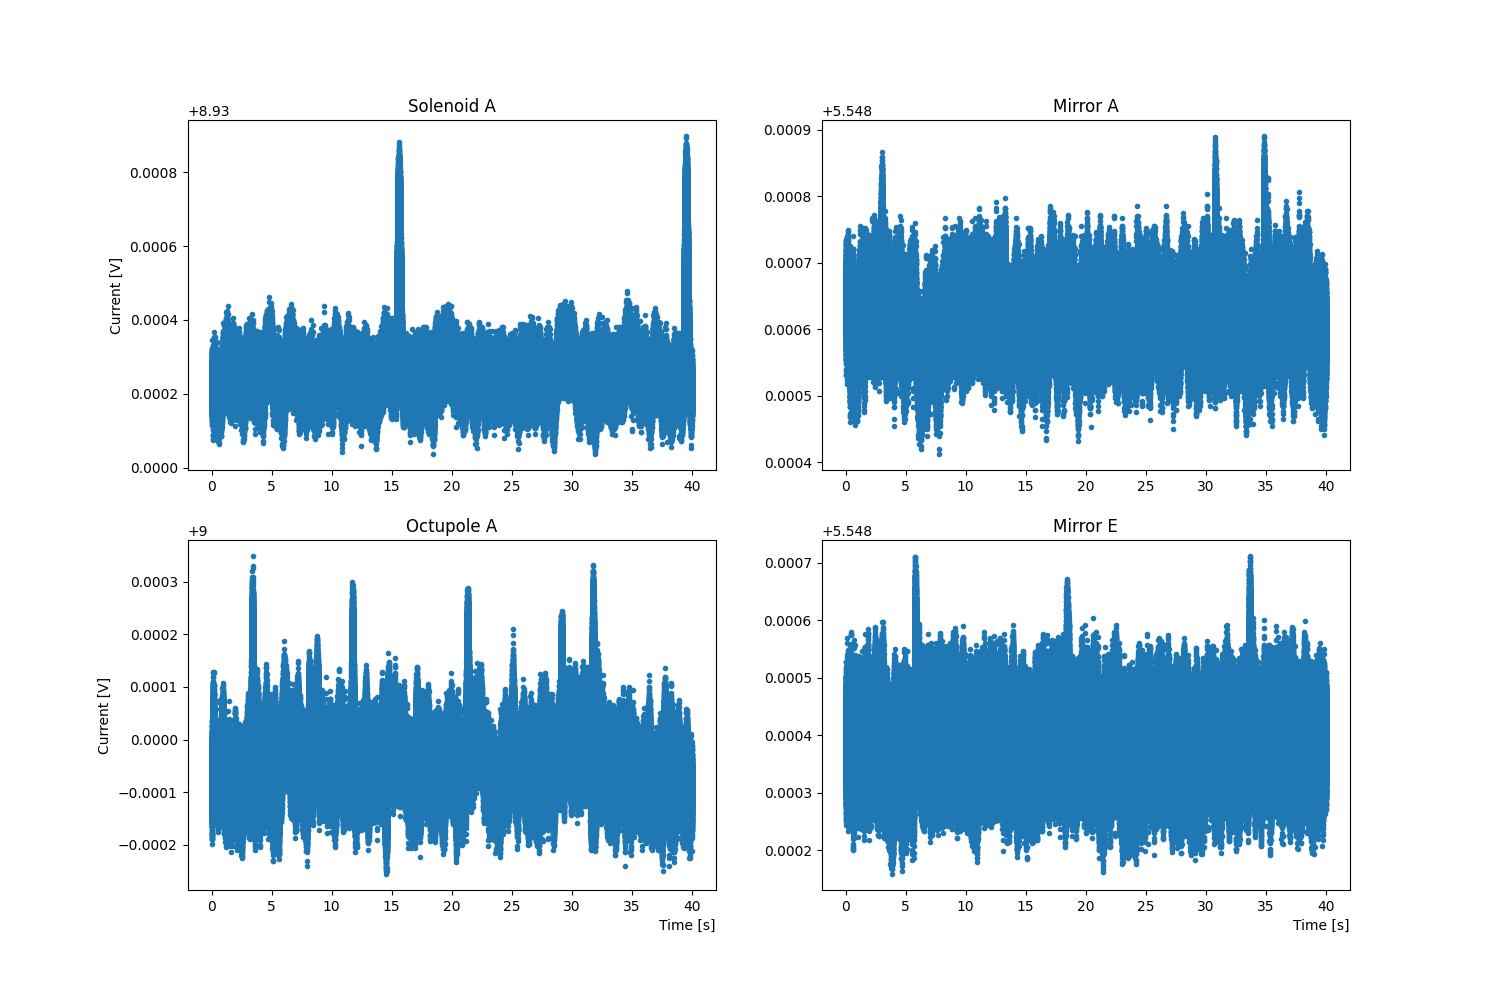
\includegraphics[width = \textwidth]{figures/chapter 4/Example_of_DCCTs_traces.png}
\caption{Example of DCCTs traces for a total of 40 second of acquisition. The units on the y-axis are Volts, since the DCCT provides a $\pm 10 $ V output. The traces have been converted into Ampere units and the amplitude of the glitches has been used to study possible discrepancies on the measurement induced by changes in the magnetic field minimum.}
\label{fig:DCCTsTraces}
\end{figure}

As evident in Fig.~\ref{fig:DCCTsTraces}, the DCCT traces for a selection of magnets show that there are glitches in the magnet currents occurring on a \SI{10}{\kilo \hertz} scale. These glitches could potentially influence the magnetic field profile along the axis, which can result in a temporary (fast) change in the resonance frequency of the atoms. Although the duration of the observed glitches for all the magnets has been confirmed to be short (less than \SI{0.1}{\second}), their amplitudes, when translated into \SI{}{\kilo \hertz} units, were non-negligible (of the order of \SI{10}{\kilo \hertz}).

Such an effect can potentially displace and anticipate some of the annihilations that would occur later during the microwave scan. Hence, an ad-hoc simulation study was performed to estimate how much such displacement occurring with a certain rate would affect the hyperfine splitting measurement. 

The simulation was performed by creating pseudo-data from the real datasets. Glitches similar to the ones observed in Fig.~\ref{fig:DCCTsTraces} were simulated with a time rate of \SI{10}{\hertz}. Each time a glitch happens, it is chosen randomly from a list containing all the glitches observed during the \SI{40}{\second} of DCCT traces measured. Each glitch was approximated as a step function, with a duration fixed to be equal to the interval over which the glitch goes from $10$ percent (before peak) to $10$ percent (after peak), and an amplitude equal to the observed peak. By considering the peak, we overestimate the displacement of the annihilations. 

The simulation considers the displacement to be asymmetrical. This means that negative current glitches (where the magnetic field decreases) anticipate annihilations happening later on in the spectra, while positive glitches delay some of the annihilations to the next bin. With this simulation mechanism, pseudo-data were generated and fitted with the same nominal protocol used in the analysis. The simulation consisted of 40 pseudo-experiments, and the standard deviation of the results was used to estimate the effect on the splitting. The standard deviation of the results obtained for both series is \SI{0.7}{\kilo \hertz}, which is small compared to other systematic uncertainties. Besides this, further consideration indicates that assuming a 100 \% conversion from current to frequency displacement is a generous overestimation. In fact, because of the coupling between different magnets, the mutual induction contributes to mitigating the effect on the magnetic field profile. This computed value is to be considered as a cross-check that shows that, if such a mechanism is present, its influence on the measurement is small; hence it was not considered in the final estimation of the systematic uncertainty.

\subsection{Error Budget Table} \label{sec:ErrorBudgetSec}

This section contains the error budget table, which contains all the alternative results of the analysis by the different methodologies that have been considered for systematic studies. The first row, indicated with \textit{Nominal,(``common fit'' linear GLS)}, represents the final analysis result with the nominal parameters and methodology. The reported result is blinded, and the frequency separation used during the experiment (the separation between the \cb and \da microwave sweeps), which is equal to \SI{1420390}{\kilo \hertz}, is not added to the final result. All the remaining rows represent different analysis methodologies that have been considered to estimate the various systematic uncertainties. All results are blinded using the same blinding value, so that they all share a common offset and can therefore be directly compared; they are grouped into separate sections, according to the specific effect each alternative approach is intended to address. The systematic uncertainty is estimated from the difference between the \textit{Nominal} result and the alternative approach. This difference has been reported for each alternative approach in a separate column indicated with \textbf{$\Delta$}. For each sub-group, the maximum difference has been taken as the nominal systematic uncertainty, and is reported in summary Tab.~\ref{tab:syst}. The last column contains the combination of the two series, and the results are obtained by the weighted mean of the results of the two series using the statistical error as weight.

\begin{table}[!h]																			
\small 
\centering
\scalebox{0.8}{
\begin{tabular}{l||r|l||r|l||r|l}																			
%\hline
%\multicolumn{7}{c}{GLS COMBINED LINEAR FIT} \\
\hline								\hline		
\textbf{Configuration} & \multicolumn{2}{c||}{\textbf{High field (kHz)}} & \multicolumn{2}{c||}{\textbf{Low Field (kHz)}} & \multicolumn{2}{c}{\textbf{Combination}} \\																			
	& $	a^{blind}_{1S}/h	\pm	\sigma$ & $	\bf{\Delta}$ & $ a^{blind}_{1S}/h \pm	\sigma$ & $\bf{\Delta}$ & $ a^{blind}_{1S}/h \pm	\sigma$ & $\bf{\Delta}$ \\
\hline																			
\hline												 
{\it Nominal (``common fit'' linear GLS)} & & & & & & \\							
$k=2$, $t_{gauss}^{cb}=10$, $t_{gauss}^{da}=10$  & {\bf \textcolor{blue}{ 10.83 $\pm$ 1.7  }}  & $ - $  & { \bf \textcolor{blue}{8.98 $\pm$ 1.5}}  & $ - $ & {\bf \textcolor{blue}{9.79 $\pm$ 1.1} }  & $ - $\\
\hline 
\hline 
{\it Lineshape reproducibility} & & & & & & \\
Nominal with g from post	                     & $ 16.48 \pm 0.4 $ & $ (5.65)	 $    & $-4.98 \pm 0.4 $ & $ (-13.96) $       & $4.41 \pm 0.3$ & $-5.38$ \\
{\it $\Delta$ is divided by 2 (see text)}        &                   & $ {\bf 2.8 } $ &                  & ${\bf -7.0}$     &                & ${\bf -2.7}$ \\
\hline 
\hline
{\it bare function $g$ (choice)} & & & & & & \\
Alt. bare function, $k=2$, $t_{cusp}=6$	          & $ 11.28 \pm 1.4$ & ${\bf 0.5}$    & $9.65	\pm 0.4$ & ${\bf 0.7}$      &  $10.36 \pm 0.4$& ${\bf 0.6}$ \\
\hline
{\it (parameters)} & & & & & & \\
$k=1$& $8.32  \pm 1.0 $       & $ {\bf -2.5}$     & $9.31 \pm 0.8 $    & $ 0.3 $     & $8.88 \pm 0.6$ & ${\bf -0.9}$ \\
$k=5.4$ & $10.70 \pm 3.8 $    & $ -0.1$           & $10.01 \pm 3.2 $   & {\bf  1.0 } & $10.31 \pm 2.4$& $0.5$  \\
\nullo{$k=5.4$, $t_{gauss}^{cb}=10$, $t_{gauss}^{da}=10$}	max uncertainty increase & ($\sqrt{3.8^{2}-1.7^{2}})$ & {\bf 3.4 } & ($\sqrt{3.2^{2}-1.5^{2}})$ & {\bf 3.0} & ($\sqrt{2.4^{2} - 1.1^{2}}$) & {\bf 2.1}\\
\hline
\hline 
{\it Resolution function} & & & & & & \\
{\it (choice)} & & & & & & \\
$t_{cusp}^{cb}=t_{cusp}^{da}=5.1$	    & $11.15 \pm 1.7 $ & ${\bf 0.3 } $ & $8.99 \pm 1.4 $ & $ 0.0$       & $ 9.94 \pm 1.1$ & $0.2$ \\
$t_{gauss}^{cb}=t_{gauss}^{da}=13.6$	& $11.00 \pm 1.9 $ & $ 0.2 $       & $9.22 \pm 1.6 $ & $ 0.2 $      & $10.00 \pm 1.2$ & $0.2$ \\
$t_{gauss}^{cb}=t_{gauss}^{da}=7.0$	    & $10.9  \pm 1.6 $ & $ 0.1 $       & $9.62 \pm 1.4 $ & $ {\bf 0.6}$ & $9.83  \pm 1.1$ & ${\bf 1.1}$  \\
\hline
{\it (frequency marker)} & & & & & & \\
$t_{gauss}^{cb}=10$, $t_{gauss}^{da}=8$	 & $7.64 \pm 1.7 $   & $ -3.2$      & $5.87 \pm 1.5 $   & $ -3.1$       & $6.64 \pm 1.1$ & $-3.2$ \\
$t_{gauss}^{cb}=10$, $t_{gauss}^{da}=12$ & $14.34 \pm 1.8 $  & ${\bf 3.5 }$ & $12.35 \pm 1.5 $  & $ 3.4$        & $13.22 \pm 1.2$& ${\bf 3.4}$  \\
$t_{gauss}^{cb}=8$, $t_{gauss}^{da}=10$	 & $13.75 \pm 1.7 $  & $ 2.9 $      & $12.45 \pm 1.4 $  & $ {\bf 3.5 }$ & $13.02 \pm 1.1$& $3.2$  \\
$t_{gauss}^{cb}=12$, $t_{gauss}^{da}=10$ & $7.43 \pm 1.8 $   & $ -3.4 $     & $5.74 \pm 1.5 $   & $ -3.2$       & $6.48 \pm 1.2$ & $-3.3$ \\
$t_{gauss}^{cb}=t_{gauss}^{da}=0$        & $11.97 \pm 1.6 $  & $ 1.1$       & $9.89 \pm 1.3 $   & $0.9 $        & $10.80 \pm 1.0$& $1.0$   \\
\hline 
\hline
{\it B-drift} & & & & & & \\	
{\it (fit procedure)} & & & & & & \\	
``split'' linear                           & $8.49 \pm 1.7$ & ${\bf -2.3}	$& $9.51 \pm 1.5$ & $ {\bf +0.5}	$& $9.06 \pm 1.1$ & ${\bf -0.7}$ \\
\hline 
{\it (long time scale linearity)} & & & & & & \\	
``split'' linear vs. ``split'' GPR         &  $8.24 \pm 1.7$  & ${\bf -0.3}	$&$9.43 \pm 1.5$   & $ {\bf -0.1}	$& $8.91 \pm 1.1$ & ${\bf -0.2}$ \\
\hline 
{\it (short time scale drift)} & & & & & & \\	
2023 specific data & N/A & ${\bf 1.1} $ & N/A & $ {\bf 1.1} $ & N/A & $ {\bf 1.1} $ \\
\hline
\hline 
{\it Data selection and binning} & & & & & & \\
Annihilation time shifted by 30 ms	       & $10.84 \pm 1.7 $  & $0.0$ &  $8.98 \pm 1.5 $ & $	0.0	$ & $ 9.79 \pm 1.1$  & $ - $\\
Binning                                    & N/A & ${\bf 2.0}$ & N/A   & ${\bf 2.0 }	$ & N/A  &  ${\bf 2.0 }$\\
\hline
\hline 
{\it Cross checks} & & & & & & \\
Nominal without $\mu$w transition veto	   & $10.93 \pm 1.7 $  & $ 0.1 $    & $8.89 \pm 1.5 $  & $ -0.1 $ & $ 9.78 \pm 1.1$  & $ - $\\
\hline
\hline
\end{tabular}
}
\caption{Results of the nominal maximum likelihood fit. The results are blind (see Eq.~\ref{eq:deltaf}). For the alternative configurations used to evaluate the systematic uncertainties, the difference $\Delta$ with respect to the results of the nominal fits are reported. The $\Delta$ values shown in {\bf bold}, are the ones summed in quadrature to obtain the total systematic uncertainty reported in Tab.~\ref{tab:syst}.
\label{tab:results}}								
\end{table}

\section{Validation and Cross-Checks of the Analysis} \label{checks}

\subsection{Rise Parameters Free to Vary from Repetition to Repetition}

The fit procedure has been thoroughly described in Sec.~\ref{sec:MLEfit}. The parameters of the fit regarding the rise of the line-shape were common for all the repetitions of a given transition. This was done under the assumption that the shape remains the same during the period of time of the Series data taking. A systematic uncertainty was estimated for this assumption in Sec.~\ref{sec:Reproducibility}. As a cross-check, this requirement was relaxed and the 8 repetitions were allowed to have different rise widths (via the $\sigma$ parameter). The values of the rise length, for the \cb and for the \da transitions, are reported in Fig.~\ref{fig:free_rise} for the two series. With this configuration, the values of $\mu = \langle\Delta f^i \rangle$ and of the corresponding standard deviation are:
\begin{itemize}
    \item \textbf{high field (\SI{1.07}{\tesla})}: $ 1\,420\,404.1 \pm 1.7 \; {\mathrm{(stat)}}$,
    \item \textbf{low field (\SI{1.03}{\tesla})}: $ 1\,420\,402.2 \pm 1.4 \; {\mathrm{(stat)}}$,
\end{itemize}
yielding a combined value of $1\,420\,403.0 \pm 1.1 \; {\mathrm{(stat)}}$, which differs less than $2\,{\rm kHz}$ from the nominal result. 
%This is another way to quantify the lineshape reproducibility uncertainty reported in Tab.~\ref{tab:results}.

Floating the rise time parameter reduces the correlation among the results in different repetitions. Consequently, even if the uncertainty on the single repetition increases, the combination of the measurements yields a result of comparable statistical uncertainty as the fit with a shared rise time. This would allow the removal of a source of systematic uncertainty (``reproducibility''), potentially at the price of fit stability. The nominal analysis has followed the configuration with the shared rise time, and this alternative estimation is left as a cross-check of the systematic related to reproducibility.


\begin{figure}[htbp]
    \centering
    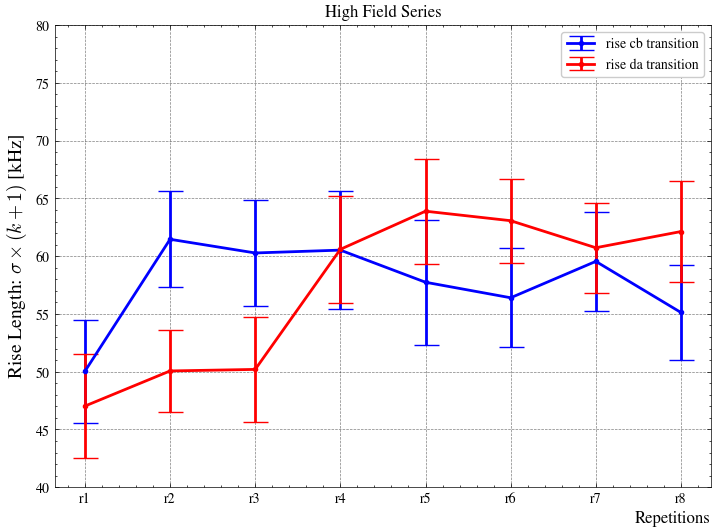
\includegraphics[width=0.75\linewidth]{figures/chapter 4/rise_s7.png} \\
    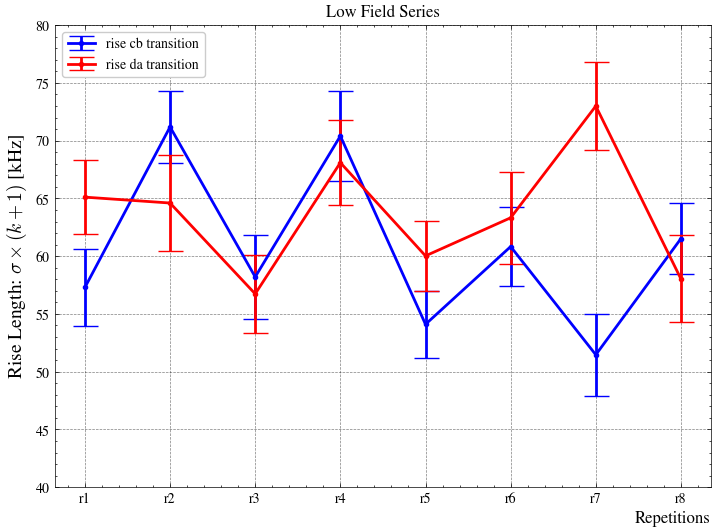
\includegraphics[width=0.75\linewidth]{figures/chapter 4/rise_s8.png}
    \caption{Length of the rising edge when letting it vary repetition by repetition (not the nominal configuration).}
    \label{fig:free_rise}
\end{figure}

\subsection{Peak frequency marker}

In this chapter, an uncertainty source was identified as the one associated with the frequency marker itself. This systematic uncertainty has been evaluated by changing the broadening of the resolution function as explained in sec \commento{aggiungere rimando}. As a cross-check, this uncertainty was estimated by repeating the measurement, but using the peak of the spectra as the frequency marker, and calculating the difference between results in the two cases. 

In fact, the peak of the spectra is likely to be more sensitive to power variations of the injected microwave in the trap, such as those that could affect \cb and \da differently. And, as explained before, such differences between \cb and \da directly constitute a systematic uncertainty.

The result of the analysis with this different method is:

\begin{itemize}
\item For low  field series: $a_{1S}/h$ = \SI{1420406.2}{\kilo\hertz}
\item For high field series: $a_{1S}/h$ = \SI{1420405.6}{\kilo\hertz}
\end{itemize}

These values give an uncertainty smaller than the one that was used for the error budget. Since this represents a worst-case scenario, this adds confidence that this contribution is under control.

\subsection{Z and Radius variable selection}

A validation has been performed by applying a $Z$ and radius selection in addition to the MVA classifier already considered. The analysis has been repeated for two complementary $Z$ cut selections, considering firstly all the annihilations above the mean of the Z distribution and secondly the ones below (see Fig.~\ref{fig:ZcutSelection}). This test was carried out to search for inconsistencies in the annihilation pattern, and the results obtained are compatible with one another, indicating no evidence of a dependence of the analysis result on the Z variable at the current resolution level.
A similar study was conducted using alternative radius cuts. Radius selections can help reveal possible contributions from residual-gas annihilations, which are expected to occur at a smaller radius than induced spin-flip annihilations: residual-gas annihilations can happen anywhere inside the trap volume, whereas spin-flip annihilations occur on the trap wall, at a larger value. Naturally, due to detector resolution, the reconstructed radius distribution is smeared between these two regimes, blurring the distinction. A summary of these studies is contained in Tab.~\ref{tab:selections}


\begin{figure}[!hbtp]
\centering
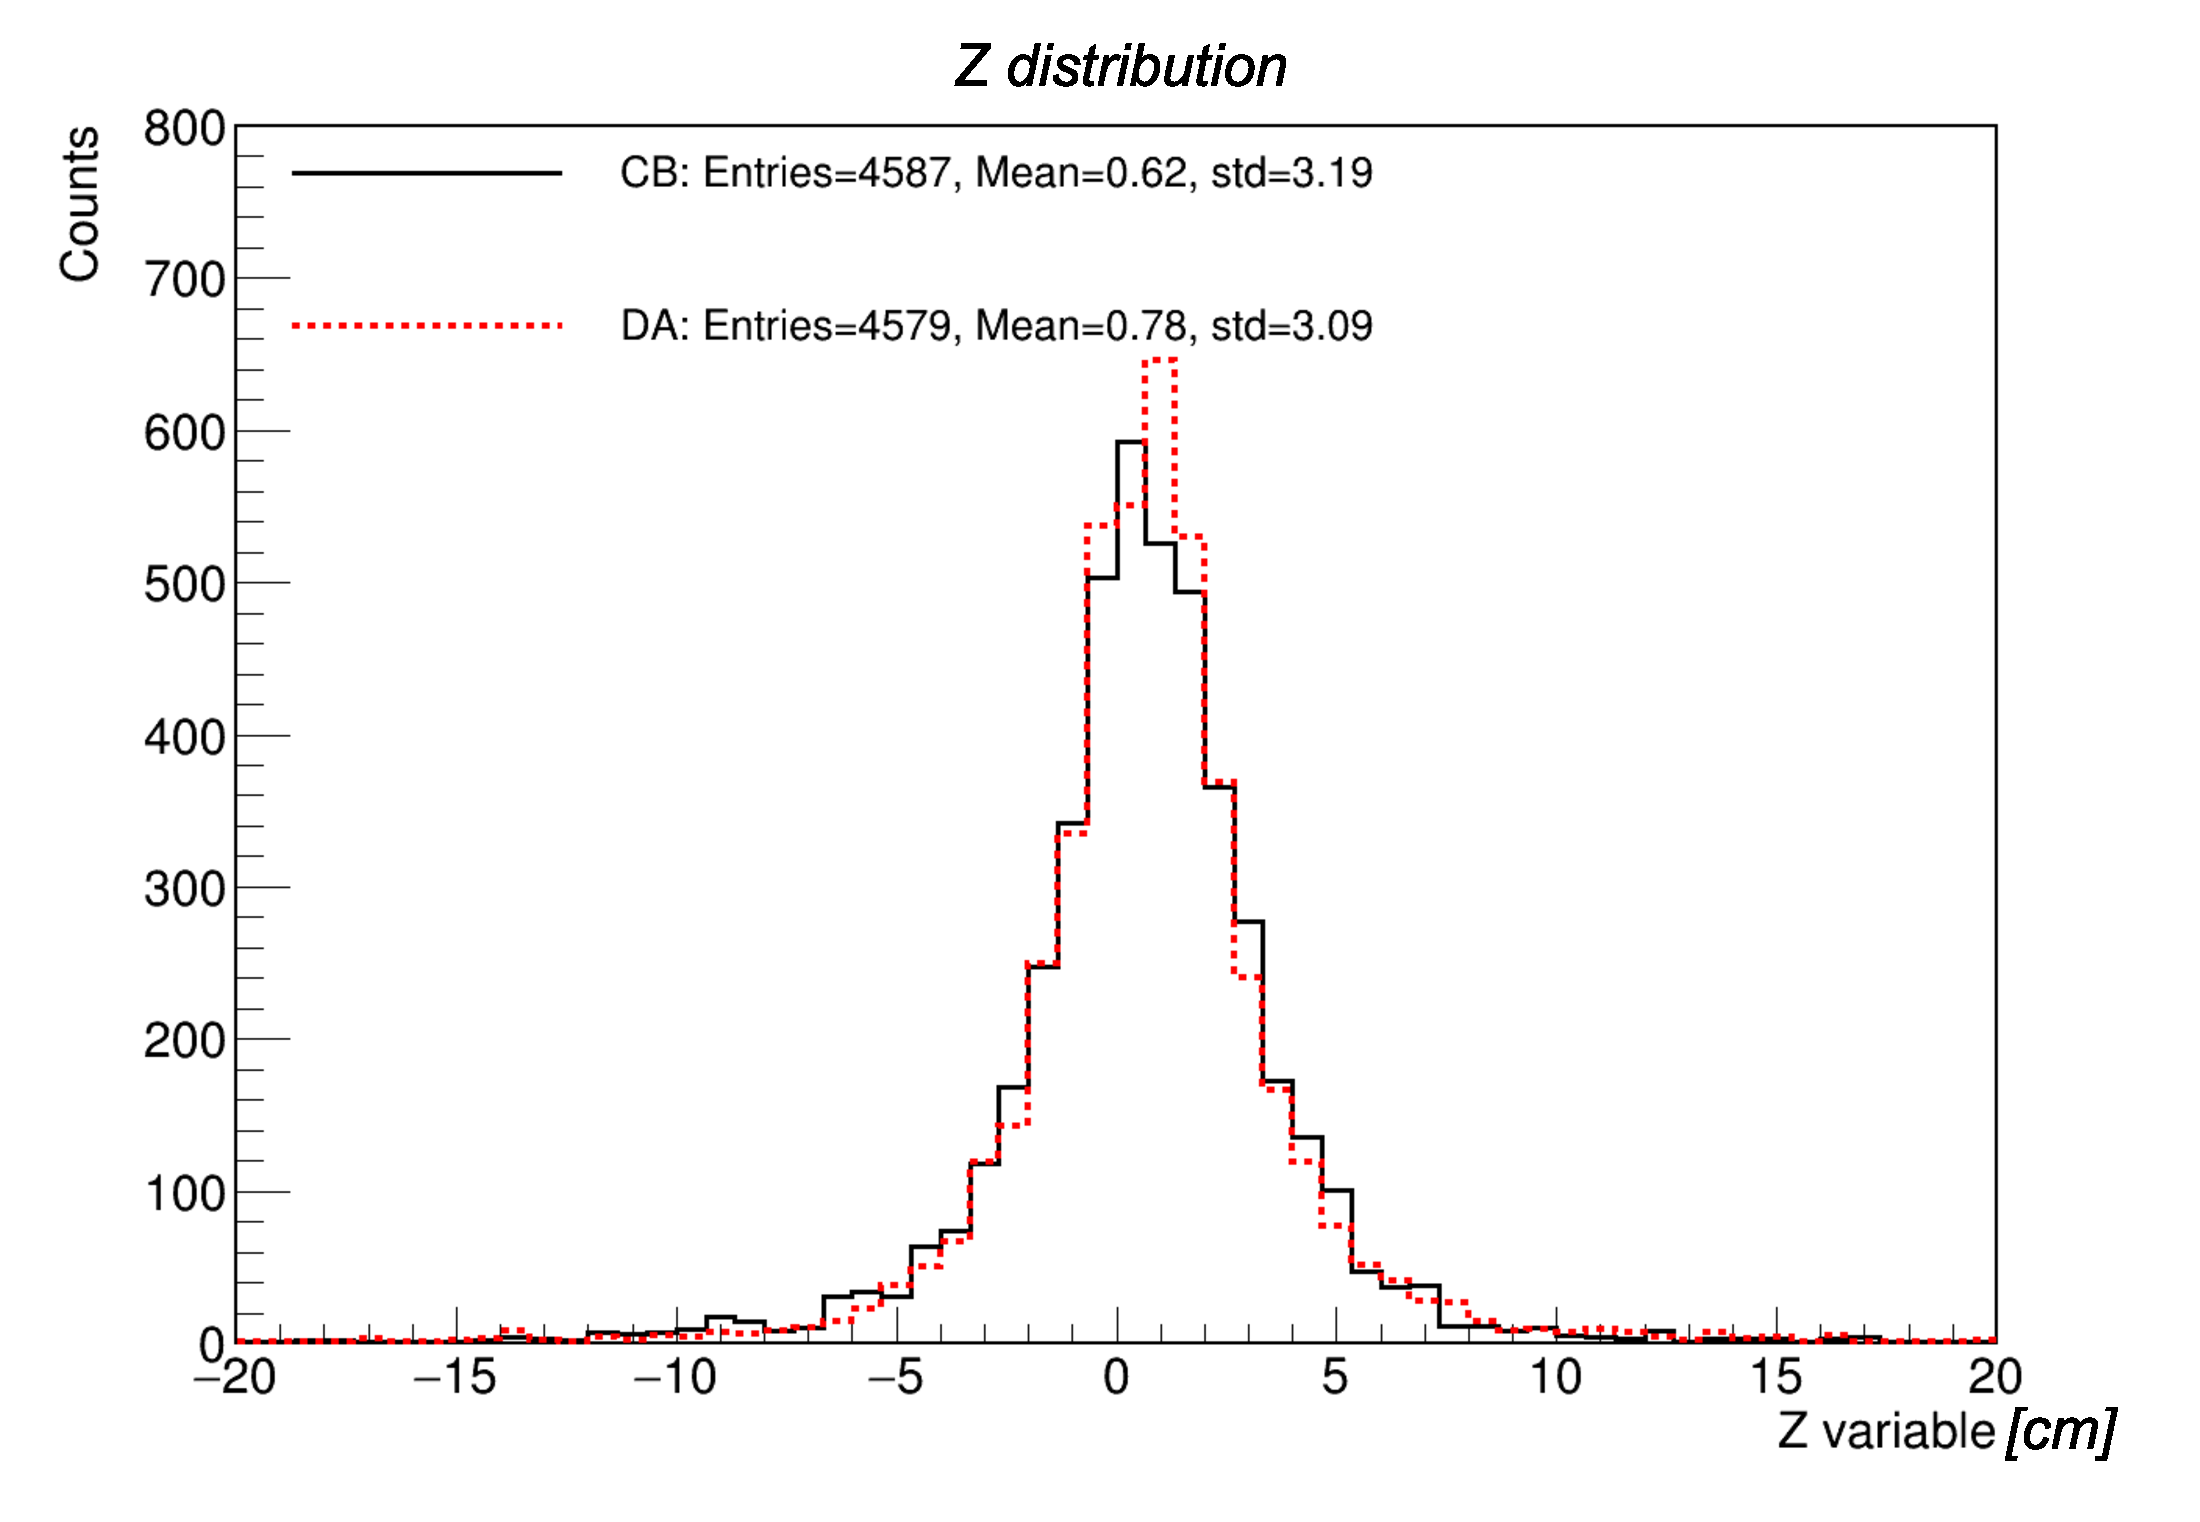
\includegraphics[width = 0.95\textwidth]{figures/chapter 4/Z_s7.pdf} \\
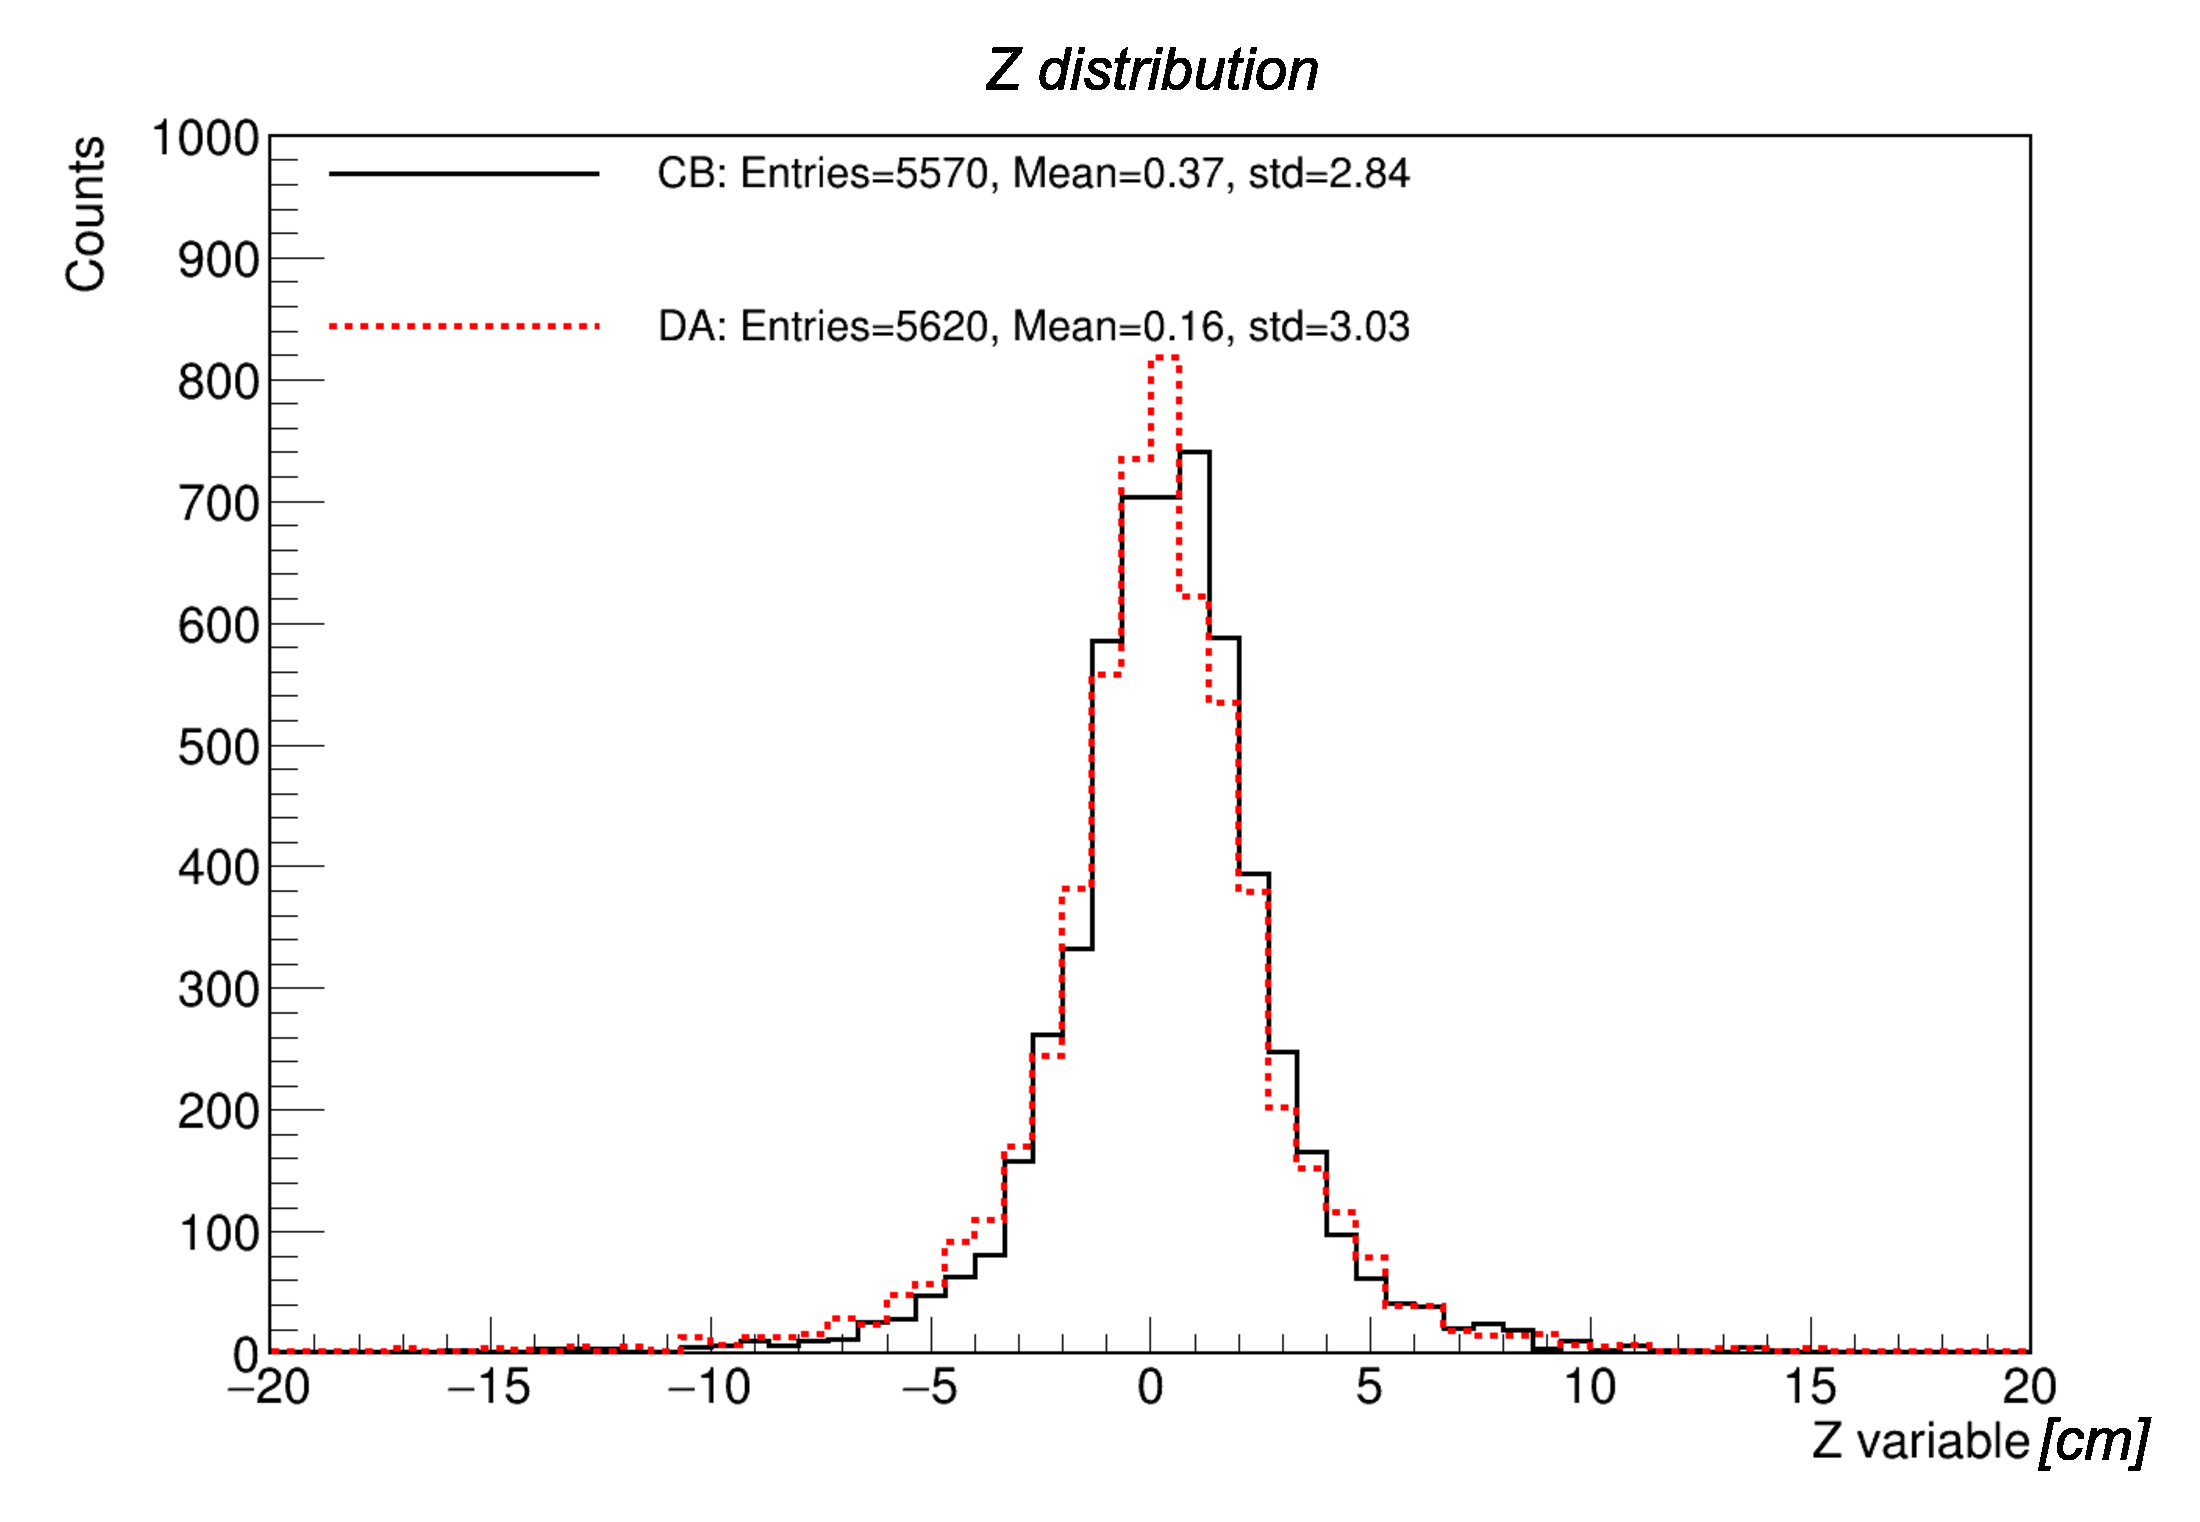
\includegraphics[width = 0.95\textwidth]{figures/chapter 4/Z_s8.pdf}
\caption{Distribution of the $Z$ variable of the annihilation vertices for the high field series (top plot) and low field series (bottom plot). Each plot shows two distributions: the $Z$ distribution for annihilations during the \cb measurement (black continuous line) and during the \da measurement (red dotted lines). The distribution contains all the accumulated events of the eight repetitions.}
\label{fig:ZcutSelection}
\end{figure}



\begin{table}[!h]
\centering							
\begin{tabular}{l||r|l||r|l}					
\hline
\hline								
\textbf{Configuration} & \multicolumn{2}{c||}{\textbf{\SI{1.07}{\tesla} dataset}} & \multicolumn{2}{c}{\textbf{\SI{1.03}{\tesla} dataset}} \\
 & $	\mu	\pm	\sigma \;({\rm kHz})$ & $	\bf{\Delta}	\;({\rm kHz})$ & $	\mu	\pm	\sigma	\;({\rm kHz}) $ & $	\bf{\Delta}	\;({\rm kHz})$ \\
\hline
\hline
{\bf \textcolor{blue}{Nominal}}	& {\textcolor{blue}{10.84 $\pm$ 1.7}} &$- $& {\textcolor{blue}{8.98 $\pm$ 1.5 }}& $ - $ \\
\hline
\hline
$1.5< r< 4\,{\rm cm}$ & $ 10.09 \pm 1.9 $ & $ -0.8 $& $ 6.95 \pm 1.7 $ & $ -2.03  $ \\
$ |z|<5\,{\rm cm}$    & $9.65 \pm 1.7$ & $-1.2 $& $9.92 \pm 1.5$ & $ +1.0 $ \\
\hline
\hline
 $Z_{cb} > 0.62 $ \& $Z_{da} > 0.78$ & $ 12.3 \pm 2.4 $ & $ 1.4$ & N/A & N/A\\
 $Z_{cb} < 0.62 $ \& $Z_{da} < 0.78$ & $ 9.9 \pm 2.4  $ & $-0.9$ & N/A & N/A\\
\hline
 $Z_{cb} >$ 0.37  \& $Z_{da} > 0.16$ & N/A & N/A & $8.00  \pm 2.1$ & $ -1.0 $ \\
 $Z_{cb} <$ 0.37  \& $Z_{da} < 0.16$ & N/A & N/A & $10.32 \pm 2.0$ & $ +1.3$\\

\hline
\hline
\end{tabular}
\caption{Comparison of the results with geometrical selections. The results reported in the table are blinded. The Nominal value corresponds to the blind result of the analysis. The systematic shift is the result of the difference between the values reported in the nominal row and the other values reported in the following rows.}
\label{tab:selections}
\end{table}



\chapter{Results Summary}
\label{ch:results}

In the previous chapter we have presented the data analysis that was performed on the 2024 data to extract the hyperfine splitting of the antihydrogen atom. The analysis has been developed with blinded results, and the unblinded results have been revealed in a confidential collaboration meeting in the early months of 2025.

The hyperfine splitting has been measured for the two different datasets, and the final results are:

\begin{equation*}
a^{\text{high field}}_{1S}/h = 1420405.8 \pm 1.7\,(\text{stat}) \pm 7.0\,(\text{syst}) \; \text{kHz}
\end{equation*}

for the dataset taken at higher magnetic field values (\SI{1.07}{\tesla}), while 

\begin{equation*}
a^{\text{low field}}_{1S}/h = 1420403.9 \pm 1.5\,(\text{stat}) \pm 8.8\,(\text{syst}) \; \text{kHz}
\end{equation*}

for the dataset taken at lower magnetic field values (\SI{1.03}{\tesla}). The two values have been statistically combined, with a weighted mean, combining also the systematic error of the two series (as explained in Sec.~\ref{sec:ErrorBudgetSec}). To date, this represents the most precise determination of the hyperfine splitting of the ground state of the antihydrogen atom. This experimental result has been published in Nature journal \cite{ALPHA:2026lbu}. The published value is:

\begin{equation*}
a_{1S}/h = 1420404.8 \pm 1.1\,(\text{stat}) \pm 5.6\,(\text{syst}) \; \text{kHz}
\end{equation*}

The remainder of this chapter summarizes the results of the analysis and compares the method with the one adopted in the previous measurement. It then briefly discusses how this measurement fits into the broader context of antimatter tests of physics beyond the Standard Model, and closes with an outlook on future developments.   

\subsection{Residuals}

In this section we report the residuals of the measured splitting of each repetition individually. The plot contains 16 points, 8 for the low field series and 8 for the high field series. The x-axis contains the microwave frequency of the first bin of the scan for the \cb transition $f_{cb}^{(i)}$. The zero on the x-axis corresponds to the mean value of the 16 $f_{cb}^{(i)}$ points. The 8 points on the left represent the 8 repetitions of the low field series, while the 8 points on the right belong to the series at high field. Given in frequency units, the distance between the two series is about \SI{1.190}{\giga\hertz}.

Each individual splitting can be written as:

\begin{equation}
a_{1S}^{(i)}/h = f_{da}^{(i)}(t + \delta t) - f_{cb}^{(i)}(t)
\end{equation}
 
To have a meaningful plot, the magnetic drift must be corrected. So $m \delta t$ is subtracted from each $a_{1S}^{(i)}/h$, giving the drift-corrected values $a_{1S,\,corr.}^{(i)}/h$, using the values of the slope obtained in Tab.~\ref{tab:resultsBdrift}. The residuals are then computed with respect to the average value of the 16 points,

\begin{equation}
\Delta f^{(i)}_{drift corr.} = \frac{a_{1S,\,corr.}^{(i)}}{h} - \frac{1}{n} \sum_{j=1}^{j=16} \frac{a_{1S,\,corr.}^{(j)}}{h}
\end{equation}

and are plotted in Fig.~\ref{fig:ResidualPlot}. The purpose is to demonstrate that there is no structured trend attributable to the magnetic field, which would otherwise suggest a dependence of the hyperfine splitting on the absolute magnetic field.

\begin{figure}[!hbtp]
\centering
\includegraphics[width= \textwidth]{figures/chapter 4/hfspairs.png}
\caption{Pair splitting residuals for each repetition for the two sets of data. The residuals $\Delta f^{(i)} = f^{(i)}_{da} - f^{(i)}_{cb}$ are corrected for the magnetic field drift and plotted with respect to the common average of both transitions (average over 16 values). 
The \textit{uncertainty} bands shown, where blue is for the statistical and red for the systematic one, refers (respectively) to the quadrature sum of the stat. uncertainty of $f^{(i)}_{da}, f^{(i)}_{cb}$ (reported in Tab.~\ref{tab:resultsf0}, with a CL of 68 \%), and the combined systematic uncertainty of the individual data-set (reported in Tab.~\ref{tab:syst}).}
\label{fig:ResidualPlot}
\end{figure}

\section{Table of Results}

Tab.~\ref{tab:resultsBdrift} contains the numerical values of the residuals from the linear common fit extraction, as discussed in Sec.~\ref{sec:CommonFitExtraction}. The table contains the magnetic field decay $m$ determined with the two methods (``common'' fit and ``split'' method, see Sec.~\ref{sec:decaySystematic}), with the first one used in the nominal approach and the latter for systematic evaluation.

\begin{table}[h]
\centering
\resizebox{\columnwidth}{!}{
\begin{tabular}{l|cc|cc}
\hline
\hline
\textbf{Residuals (kHz)} & \textbf{\SI{1.07}{\tesla}} dataset (\cb)  & (\da) & \textbf{\SI{1.03}{\tesla}} dataset (\cb) & (\da) \\ 
\hline 
$\Delta t$ (s) & \multicolumn{2}{c|}{812.4} & \multicolumn{2}{c}{812.4} \\
\hline \hline 
$m_{common}$ (kHz/h) & \multicolumn{2}{c|}{$-75.64 \pm 0.05$} & \multicolumn{2}{c}{$-72.82 \pm 0.04$} \\
\hline 
r0 & $ -16.4 \pm 1.5 $ & $ -15.8 \pm 1.5 $ & $ 6.8 \pm 1.2 $ & $ 0.9 \pm 1.2 $ \\
r1 & $ -0.3 \pm 1.5 $ & $ -0.9 \pm 1.5 $ & $ 6.0 \pm 1.2 $ & $ 3.3 \pm 1.2 $ \\
r2 & $ 9.9 \pm 1.5 $ & $ 6.8 \pm 1.5 $ & $ -2.4 \pm 1.2 $ & $ -5.1 \pm 1.2 $ \\
r3 & $ 10.3 \pm 1.5 $ & $ 3.3 \pm 1.5 $ & $ -11.6 \pm 1.2 $ & $ -1.5 \pm 1.2 $ \\
r4 & $ 3.9 \pm 1.5 $ & $ 8.9 \pm 1.5 $ & $ -9.7 \pm 1.2 $ & $ -8.3 \pm 1.2 $ \\
r5 & $ -0.9 \pm 1.5 $ & $ -2.2 \pm 1.5 $ & $ -0.3 \pm 1.2 $ & $ -4.1 \pm 1.2 $ \\
r6 & $ -2.0 \pm 1.5 $ & $ -7.5 \pm 1.5 $ & $ 3.1 \pm 1.2 $ & $ 9.3 \pm 1.2 $ \\
r7 & $ -0.0 \pm 1.5 $ & $ -10.7 \pm 1.5 $ & $ 5.7 \pm 1.2 $ & $ 2.9 \pm 1.2 $ \\
\hline \hline
$m_{split}$ (kHz/h) & $-75.3 \pm 0.1$  & $-75.9 \pm 0.1$ & $-73.0 \pm 0.1$ & $-72.6 \pm 0.1$\\
%$m_{da}$ (kHz/h) & &  & $-72.6 \pm 0.1$ & $-72.6 \pm 0.1$ \\
%$m_{avg}$ (kHz/h) & $-75.6 \pm 0.1$   & $-75.6 \pm 0.1$ & $-72.8 \pm 0.1$ & $-72.8 \pm 0.1$ \\
\hline
\hline
\end{tabular}
}
\caption{$B$-drift correction parameters and residuals from the common linear fit. The $\Delta t (s)$ value is the time interval between the \fcb and \fda measurement.
\label{tab:resultsBdrift}}
\end{table}


\subsection{Uncertainty Table}

Tab.~\ref{tab:syst} summarizes all the main uncertainties, which have been determined by selecting the greatest contribution from every block in the error budget table (Tab.~\ref{tab:results}). The total systematic uncertainty has been determined as the quadrature sum of each individual contribution. The combination of the two analyzed dataset has been obtained from the sum of the individual shift of each row in Tab.~\ref{tab:results}, and the total systematic uncertainty of \SI{5.6}{\kilo \hertz} is the resulting from the quadrature sum of each individual contribution. This procedure has been followed to consider possible correlation between the uncertainty of each dataset. The final uncertainty can also be estimated considering the error propagation formula of two independent measurement $$\bar{x} = \frac{x/\sigma_x^2 + y/\sigma_y^2}{1/\sigma_x^2 + 1/\sigma_y^2}, \qquad \sigma_{\bar{x}} = \left(\frac{1}{\sigma_x^2} + \frac{1}{\sigma_y^2}\right)^{-1/2}$$

the result considering uncorrelation is $\sigma_{TOT} = 5.5 $ kHz, in agreement with the nominal estimation of $5.6$ kHz.

\begin{table}[!h]
\centering
\resizebox{\columnwidth}{!}{
\begin{tabular}{r|c|c|c}
\textbf{Source}  & \textbf{\SI{1.07}{\tesla} series}  (kHz) &  \textbf{\SI{1.03}{\tesla} series}  (kHz) & \textbf{Combination}\\
\hline \hline
%\textbf{Statistical} & \textbf{-} & \textbf{-} & \textbf{-}\\
%\hline \hline
Line-shape reproducibility                & 2.8 & 7.0 & 2.7\\
\hline
Bare function ({\it choice})                   & 0.5 & 0.7 & 0.6\\
Bare function ({\it parameters})               & 2.5 & 1.0 & 0.9\\
Bare function ({\it uncertainty increase})     & 3.4 & 3.0 & 2.1\\
\hline
Resolution function ({\it choice})             & 0.3 & 0.6 & 1.1\\
Resolution function ({\it frequency marker})   & 3.5 & 3.5 & 3.4\\
\hline
B-drift ({\it fit procedure})                  & 2.3 & 0.5 & 0.7\\
%\hline
B-drift ({\it long time scale linearity})      & 0.3 & 0.1 & 0.2\\
%\hline
B-drift ({\it short time scale linearity}) & 1.1 & 1.1 & 1.1\\
\hline
Data selection and binning               & 2.0 & 2.0 & 2.0\\
\hline
\hline
\textbf{Total systematic}                & 7.0 & 8.8 & 5.6\\
\end{tabular}
}
\caption{Summary of the uncertainties associated to the measurement of the hyperfine splitting.
\label{tab:syst}}
\end{table}


\section{Comparison with the 2017 measurement} \label{sec:comparison2017}

The present result improves on the first measurement of the antihydrogen ground-state hyperfine splitting, $1\,420.4 \pm 0.5$~MHz \cite{ALPHA:2017fsh}, by about two orders of magnitude. The gain does not come from a single change, and it is useful to separate the improvements in the experimental conditions from those in the analysis.

On the experimental side, the 2017 measurement was based on 194 detected atoms collected in 22 trials over three days, with \SI{300}{\kilo\hertz} frequency steps of \SI{4}{\second} each, in an unflattened trapping field \cite{ALPHA:2017fsh}. The present one uses about 24\,000 atoms, accumulated with the Be$^+$-assisted scheme \cite{Akbari:2025mli}, \SI{5}{\kilo\hertz} steps of \SI{8}{\second}, and a magnetic field profile whose second axial derivative is about 20 times smaller \cite{ALPHA:2026lbu}, which increases the interaction time of the atoms with the microwaves near the field minimum (Sec.~\ref{sec:MagFieldProfile}). The microwave power at the two transitions was balanced with dedicated lineshape studies, and the field drift was characterized with ECR and corrected with a common fit to the 16 frequency markers of each series. In 2017, each of the field drift during the scan, the combination of data from different days and the determination of the onsets contributed \SI{0.3}{\mega\hertz} to the uncertainty \cite{ALPHA:2017fsh}.

On the analysis side, the main change is in the definition of the frequency marker. In 2017 the splitting was obtained from the difference between the low-frequency onsets of the two lines. With the present statistics and resolution this is not sufficient: the onset of the observed lineshape is not the resonance at the field minimum, but is displaced by the broadening mechanisms discussed in Chapter~\ref{ch:analysis}, and the displacement can differ between the two transitions. Identifying the need for a marker that accounts for this physics, i.e.\ extrapolated back from the observed rising edge and defined consistently with the broadening, was the first and most important step, and it had not been considered in the previous measurement.

The second step was the choice of the method to implement it. During the preliminary phase of the analysis, which preceded the data taking itself, the statistical and systematic performance of different strategies was studied with Monte Carlo pseudo-experiments. These studies showed that a simple threshold-crossing criterion, in which the onset is identified as the first frequency bin with more than one count followed by a bin with more than two counts, is not robust for a dataset of this kind, and that among the algorithms tested the one used in the previous analysis gave the worst performance. Other approaches would have been possible, for instance a constant-fraction crossing followed by a correction for the broadening, but fitting the spectra with a lineshape model convolved with a resolution function turned out to be more convenient: the fit incorporates the onset definition, the broadening and the background in a single procedure, which makes it possible to study all the systematic uncertainties in a unified way (Chapter~\ref{ch:analysis}).

\section{CPT and outlook} \label{sec:outlookthesis}

This recent result from the \ALPHA collaboration allows a direct comparison with the most precise determination of the ground state hyperfine level on hydrogen for testing CPT invariance in a model-independent test. While the agreement between the antihydrogen and hydrogen ground-state hyperfine splitting constitutes a stringent, model-independent test of CPT symmetry, any measurable discrepancy would directly signal CPT violation, without reference to any specific theoretical framework. Considering the current uncertainty of the measurement, dominated by the \SI{5.6}{\kilo \hertz} systematic contribution, one can determine:

\begin{equation}
\frac{\delta a_{1S}^{\overline{\mathrm{H}}}}{a_{1S}^{\overline{\mathrm{H}}}} =\frac{5.6 \; kHz}{1420404.8 \; kHz} \approx 4 \times 10^{-6} 
\end{equation}

At the current 4 ppm level of precision, the uncertainty on the antihydrogen ground state hyperfine splitting is now well below the corrections arising from the charge and magnetization distribution of the antiproton, analogous to the well-known proton structure (Zemach radius) which for hydrogen causes a finite size shift of about $-32$ ppm \cite{Widmann_2022,PhysRevA.78.022517}. It is possible to disentangle nuclear structure correction with pure QED contributions by using a separate measurement, the hyperfine splitting of the 2S energy level. The difference $D_{21} = 8 a_{2S} - a_{1S}$, which is called Sternheim interval, has the property of largely cancelling out the nuclear structure terms, isolating an independent quantity for precision QED tests \cite{Sternheim:1963zz}. With this most recent result, the Sternheim interval for antihydrogen has been determined with a new precision:

\begin{equation*}
(8 a_{2S} - a_{1S}) / h = 100 \pm 150 \; kHz
\end{equation*}

where the precision is now limited by the measurement of the 2S hyperfine splitting, which is $a_{2S}/h = 177563 \pm 18$ kHz \cite{ALPHA:2026lbu}. The latter was first determined by combining laser spectroscopy of the two accessible hyperfine components of the 1S-2S transition with the previous \ALPHA determination of the ground-state splitting; the present result improves it by a factor 26, \cite{Baker:2025hfs,ALPHA:2026lbu}. The current determination on hydrogen, predicted by QED, leads to $48.9592 \pm 0.0068 \; kHz$ \cite{PhysRevLett.130.203001}, and shows good agreement with the new determination on antihydrogen.

Within the Standard-Model Extension (SME) \cite{ColladayKostelecky1997,ColladayKostelecky1998}, however, the observable reported here has no leading-order sensitivity to Lorentz- or CPT-violating coefficients, and this is a direct consequence of the way it is constructed: the transitions exploited drive the atom from a trapped, low-field-seeking state into an untrapped, high-field-seeking one, and the hyperfine constant is obtained by combining two such field-dependent resonances so as to cancel the local trapping field. The sensitivity of hydrogen and antihydrogen transitions to the various SME coefficients, including the ground-state Zeeman-hyperfine transitions studied in this work, was investigated in \cite{Bluhm_1999,Kostelecky:2015nma}.

\subsection{SME coefficients and hyperfine measurement}

To provide better context, we firstly introduce the modified Dirac equation for the spectra of free $\bm{H}$ and $\bm{\overline{H}}$. This is useful to introduce the specific coefficients towards which a potential comparison between hydrogen and antihydrogen is sensitive to. The modified Dirac equation for an electron/positron field is the following:

\begin{equation}
(i \gamma^{\mu} - m_{e} - a^{e}_{\mu} \gamma^{\mu} - b^{e}_{\mu} \gamma_{5}\gamma^{\mu} - 1/2 H^{e}_{\mu \nu} \sigma^{\mu \nu} + i c^{e}_{\mu \nu} \gamma^{\mu} D^{\nu} + i d^{e}_{\mu \nu} \gamma_{5}\gamma^{\mu} D^{\nu})\psi = 0
\end{equation}

It is beyond the scope of the thesis to give a physical explanation of each new term appearing in the modified Dirac equation, but it is important to highlight what are the consequence of the presence of these new terms: for $a^{e}_{\mu}$ and $b^{e}_{\mu}$, they violate CPT symmetry, and all the five terms $a^{e}_{\mu},b^{e}_{\mu},H^{e}_{\mu \nu},c^{e}_{\mu \nu},d^{e}_{\mu \nu}$ break Lorentz invariance. A similar equation with corresponding new terms (that will be indicated with apex ``\textit{p}'' instead of ``\textit{e}'') also exists for a free antiproton.

The presence of these extra-terms produces a shift in the energy levels of hydrogen and antihydrogen. For the hydrogen case, a general formula for the 1S and 2S energy levels is:

\begin{align}
\Delta E^{H} \approx &(a_{0}^{e} + a_{0}^{p} - c^{e}_{00} m_{e} - c^{p}_{00} m_{p}) \\
 & + (-b^{e}_{3} + d^{e}_{30} m_{e} + H^{e}_{12}) \frac{m_{J}}{|m_{J}|} \\
 & + (-b^{p}_{3} + d^{p}_{30} m_{e} + H^{p}_{12}) \frac{m_{I}}{|m_{I}|}
\end{align}

where $J$ and $I$ are the electronic and protonic angular momenta. The formula can be adapted to describe the energy shifts for the antihydrogen atoms, by changing the sign of $a{e/p}_{\mu}$, $d^{e/p}_{\mu}$ and $H^{e/p}_{\mu \nu}$.

The terms in the first line do not depend on the orientation of the spins: the coefficients $a^w_0$ and $c^w_{00}$ (with $w = e, p$) shift all the hyperfine sublevels of the atom by the same amount, and therefore cancel in any transition between them. The other two lines are the ones relevant for hyperfine spectroscopy. Each of them is the product of a combination of SME coefficients and of the sign of a spin projection along the quantization axis, $m_J/|m_J| = \pm 1$ for the electron and $m_I/|m_I| = \pm 1$ for the proton; the quantization axis is the direction of the magnetic field, and the index 3 denotes the component of the coefficients along it. It is convenient to collect the two combinations in

\begin{equation}
X_e = -b^e_3 + d^e_{30} m_e + H^e_{12}, \qquad X_p = -b^p_3 + d^p_{30} m_p + H^p_{12},
\label{eq:SMEXdef}
\end{equation}

so that the spin-dependent part of the shift reads simply $X_e\, m_J/|m_J| + X_p\, m_I/|m_I|$. The electron gains an energy $+X_e$ when its spin points along the axis and $-X_e$ when it points in the opposite direction, and the proton does the same with $X_p$. This is the same behaviour as a magnetic moment in a magnetic field: from the point of view of the atom, the spin-dependent SME terms act as two tiny additional magnetic fields.
%, fixed in space, one coupling only to the electron and one only to the proton, and both unrelated to the real trapping field.

In the ground state the two spins are coupled by the hyperfine interaction, and in a magnetic field the eigenstates are the four sublevels $\ket{a}$, $\ket{b}$, $\ket{c}$, $\ket{d}$ of Chapter~\ref{ch:hyperfine}, labelled in order of increasing energy. Two of them, $\ket{d}$ and $\ket{b}$, are pure spin states, with both spins up and both spins down respectively, and their shifts follow from the expression above: $X_e + X_p$ and $-(X_e + X_p)$. The other two, $\ket{c}$ and $\ket{a}$, are superpositions of the two configurations with opposite spins, electron up and proton down or vice versa, whose shifts are $+(X_e - X_p)$ and $-(X_e - X_p)$. The shift of a mixed state is the average of these two values, weighted by the probability of each configuration. Altogether, the four sublevels of the 1S state are shifted by \cite{Bluhm_1999}

\begin{align}
\Delta E_d &\simeq + (X_e + X_p), & \Delta E_c &\simeq + \hat\kappa \, (X_e - X_p), \nonumber \\
\Delta E_b &\simeq - (X_e + X_p), & \Delta E_a &\simeq - \hat\kappa \, (X_e - X_p),
\label{eq:SMEshifts}
\end{align}

where $\hat\kappa = \cos 2\theta_1$ expresses how strongly the states $\ket{c}$ and $\ket{a}$ are mixed, through the mixing angle $\theta_1$ defined by $\tan 2\theta_1 \simeq \SI{51}{\milli\tesla}/B$ \cite{Bluhm_1999}. At zero field $\hat\kappa = 0$: the two configurations enter $\ket{c}$ and $\ket{a}$ with equal weight, their shifts average out, and these two states are not shifted at all. In a strong field $\hat\kappa \to 1$, and $\ket{c}$ and $\ket{a}$ become pure spin states as well; at the \SI{1}{\tesla} field of the experiment $\hat\kappa \simeq 0.999$.

The same structure holds for antihydrogen. The sublevels are labelled in the same way, by their position in the Zeeman diagram, but since the magnetic moment of the positron is parallel to its spin, rather than antiparallel as for the electron, each antihydrogen sublevel has the opposite spin configuration with respect to the hydrogen sublevel with the same label. Combined with the change of sign of some of the coefficients under charge conjugation, the net result is that Eq.~(\ref{eq:SMEshifts}) applies to antihydrogen with $b^e_3 \to -b^e_3$ and $b^p_3 \to -b^p_3$ in Eq.~(\ref{eq:SMEXdef}), while $d^w_{30}$ and $H^w_{12}$ keep their sign \cite{Bluhm_1999} \footnote{This is a consequence of the fact that $m_{j}/|m_{j}|$ or $m_{I}/|m_{I}|$ change sign when considering $e^{-} \rightarrow e^{+}$ and $p^{+} \rightarrow p^{-}$, along with the change of sign of the terms $d^{w}_{30}$ and $H^{w}_{12}$ under Charge conjugation $C$.}. The CPT-odd coefficients $b^w_3$ are thus the ones that can make hydrogen and antihydrogen differ.

The effect on the two measured transitions is obtained by subtracting the shifts of the final and initial states:

\begin{align}
\delta f_{da} &= \frac{\Delta E_d - \Delta E_a}{h} = \frac{(X_e + X_p) + \hat\kappa\,(X_e - X_p)}{h}, \nonumber \\
\delta f_{cb} &= \frac{\Delta E_c - \Delta E_b}{h} = \frac{\hat\kappa\,(X_e - X_p) + (X_e + X_p)}{h}.
\label{eq:SMEfcbfda}
\end{align}

The two transitions are shifted by exactly the same amount, $[X_e(1+\hat\kappa) + X_p(1-\hat\kappa)]/h$, for any value of the magnetic field and for both hydrogen and antihydrogen, and the shift cancels in the difference $f_{da} - f_{cb}$. 
%The reason is the same that makes the difference independent of the trapping field (see the energy levels retaining the antiproton Zeeman term at the end of Chapter~\ref{ch:hyperfine}). 
%At high field both transitions are essentially a flip of the positron spin, one with the antiproton spin in one direction ($\ket{d}\to\ket{a}$) and one with the antiproton spin in the other direction ($\ket{c}\to\ket{b}$). A field acting on the positron changes the energy needed for the flip by the same amount in both cases, and a field acting on the antiproton shifts the initial and final states of each transition almost equally, whatever its direction. Only the hyperfine interaction depends on the relative orientation of the two spins, and makes the positron flip cost a different energy for the two antiproton orientations: this is what the difference $f_{da} - f_{cb}$ measures, and the SME terms considered here, which act on each spin separately, cannot contribute to it. Consistently, $f_{da}-f_{cb}$ coincides with the zero-field $\ket{F=1,m_F=0} \leftrightarrow \ket{F=0,m_F=0}$ hydrogen maser transition, which is shown in \cite{Kostelecky:2015nma} to be insensitive to Lorentz violation for operators of any mass dimension, since only transitions with $\Delta m_F \neq 0$ acquire leading-order shifts. 
The hydrogen/antihydrogen agreement reported here therefore tests the equality of the magnetic interaction between the two bound particles, including the antiproton finite-size contribution discussed above, but does not constrain at leading order any of the SME coefficients considered in \cite{Bluhm_1999,Kostelecky:2015nma}.

The individual resonances do carry SME information. \fcb and \fda are predominantly a positron spin flip: at \SI{1}{\tesla}, $\hat\kappa \simeq 0.999$, so that $f_{cb}$ and $f_{da}$ shift by $\approx 2X_e/h$, with the antiproton admixture suppressed by $1-\hat\kappa \approx 10^{-3}$. A hydrogen--antihydrogen comparison of either resonance at the same field would therefore isolate the CPT-odd coefficient $b^e_3$ of the electron sector, the CPT-even $d^e_{30}$ and $H^e_{12}$ cancelling in the difference. Exploiting this would require an independent absolute calibration of the field at the location of the atoms; with the 1 ppm accuracy of the ECR technique ($\approx$ \SI{28}{\kilo \hertz} at \SI{1}{\tesla}) the reach on $b^e_3$ would be of order \SI{e-19}{\giga \electronvolt}, several orders of magnitude weaker than the bounds already set on this sector by the comparison of the electron and positron $g$-factors in Penning traps \cite{VanDyck:1987ay}. Despite this, a more promising approach can be constituted by the $c \rightarrow d$ transition, which is mainly an antiproton spin flip. Within the SME framework, it can be shown that hydrogen and antihydrogen would exhibit sensitivity to CPT violating couplings. Specifically, as computed in \cite{Bluhm_1999,Kostelecky:2015nma}, the transition frequency are at first order approximation in $\alpha$

\begin{align}
\delta^{H}_{c \rightarrow d} &\approx ( - b_{3}^{p} + d_{30}^{p} m_{p} + H_{12}^{p}) / \pi \\
\delta^{\overline{H}}_{c \rightarrow d} &\approx ( + b_{3}^{p} + d_{30}^{p} m_{p} + H_{12}^{p}) / \pi
\end{align}

The instantaneous difference of the two transition frequencies is therefore $\Delta \nu_{c \rightarrow d} = \nu^{H}_{c \rightarrow d} - \nu^{\overline{H}}_{c \rightarrow d} = - 2 b_{3}^{p}/ \pi$, so that a measurement of the $\ket{c} \rightarrow \ket{d}$ transition, between two trapped hyperfine sublevels, would isolate the antiproton coefficient $b^{p}_{3}$. The same coefficient is probed by the BASE collaboration, through the comparison of the proton and antiproton magnetic moments in Penning traps \cite{Smorra2017}.
In the present apparatus, however, this transition cannot be driven. Being mainly an antiproton spin flip, its frequency at \SI{1}{\tesla} is of the order of \SI{650}{\mega\hertz}, far below the microwave frequencies used in this work, and the geometry of the trap does not allow radiation at such frequencies to be delivered to the atoms. A measurement of this kind would therefore require dedicated hardware, and could be the subject of future developments of the experiment.

The measurement presented in this thesis shows that the systematic uncertainties of the spectroscopy of trapped antihydrogen are under control at the level of 5--10~kHz, while the magnetic field in the trap is monitored at the level of about 1~kHz in terms of the equivalent transition frequency (Sec.~\ref{sec:ECRtecnique}). This measurement validates the control of the systematic uncertainties of the technique, and constitutes the starting point for the measurement of other quantities, such as the individual resonances or the $\ket{c} \leftrightarrow \ket{d}$ transition discussed above. These quantities are also connected to the programs of the BASE and ASACUSA collaborations, which address the same physics with different methods, namely the measurement of the antiproton magnetic moment in Penning traps \cite{Smorra2017} and of the antihydrogen hyperfine splitting in a beam \cite{Diermaier:2016fsy,Widmann_2022} with a different method. Assessing the sensitivities accessible to each of these methods is a continuation could be a continuation of the work presented in this thesis. With the ground-state hyperfine splitting of antihydrogen now measured at the level of a few parts per million, antimatter hyperfine spectroscopy has moved from a first observation to a precision technique, advancing towards the way for antihydrogen to become a test of CPT symmetry and a possible probe of physics beyond the Standard Model.

%, so that matching that reach would require an absolute frequency resolution of order \SI{0.1}{\hertz} and hence anti-atom temperatures in the \si{\micro\kelvin} range \cite{Bluhm_1999}.
%


% In addition, since the laboratory-frame coefficients rotate with the Earth, a time-averaged comparison is only sensitive to their component along the Earth's rotation axis, and a dedicated sidereal-time analysis would be needed to access the remaining components \cite{Kostelecky:2015nma}. A measurement with genuine discovery potential would instead need to target a less-constrained sector.

% Moreover, its frequency is stationary with respect to the magnetic field at $B \simeq \SI{0.65}{\tesla}$ \cite{Bluhm_1999}, which removes at first order the Zeeman broadening due to the field inhomogeneity that shapes the present lineshapes and is ultimately responsible for the dominant systematic uncertainties. Since both states are trapped, the transition must be detected through a subsequent microwave transfer to an untrapped state, a double-resonance scheme compatible with the present apparatus. Combined with a dedicated search for sidereal variation, this measurement would represent a natural and well-motivated next step toward exploiting antihydrogen hyperfine spectroscopy as a genuine probe of physics beyond the Standard Model, rather than solely as a model-independent CPT test.


\listoftables
\listoffigures

\begin{appendices}

\section{Calculation of the Fine Structure for the 1s Energy Level} \label{app:finestructure}

This appendix derives, following the perturbative approach of Cohen-Tannoudji, Diu and Lalo\"e \cite{QuantumMechanics}, the fine-structure correction to the $1s$ ($n=1$, $l=0$) ground-state energy level of the hydrogen (or antihydrogen) atom, quoted without proof in Chapter~\ref{ch:hyperfine}. As recalled there, once the hyperfine term $W_{hf}$ is set aside, the fine structure of the atom originates from three additional terms in the Hamiltonian, all of order $\alpha^2$ relative to the leading-order Bohr energy $E_n$:

\begin{equation}
H_{fs} = \underbrace{-\dfrac{p^4}{8 m_{e}^3 c^2}}_{H_{rel}} \; + \; \underbrace{\frac{1}{2m_{e}^2 c^2} \dfrac{1}{r}\dfrac{dV(r)}{dr}\, L \cdot S}_{H_{SO}} \; + \; \underbrace{\frac{\hbar^2}{8m_{e}^2 c^2} \Delta V(r)}_{H_{D}} \, ,
\end{equation}

namely the relativistic correction to the kinetic energy, the spin-orbit coupling, and the Darwin term. Since $H_{fs}$ is small compared to $H_0 = p^2/2m_e + V(r)$, its effect on the (non-degenerate, for fixed $n,l,j$) energy levels can be evaluated at first order in perturbation theory, $\Delta E_{fs} = \bra{\psi} H_{fs} \ket{\psi}$, using the unperturbed hydrogenic eigenstates. For the $1s$ state, the normalized wavefunction is

\begin{equation}
\psi_{1s}(r) = \frac{1}{\sqrt{\pi}}\, a_0^{-3/2}\, e^{-r/a_0} \, ,
\end{equation}

with $a_0$ the Bohr radius. Throughout this appendix, the fine-structure constant is used in its usual definition $\alpha = e^2/(4\pi \epsilon_0 \hbar c)$, so that the Coulomb potential and the Bohr radius can be written as $V(r) = -\alpha \hbar c / r$ and $a_0 = \hbar/(m_e c \alpha)$, and the ground-state energy is $E_1 = -\frac{1}{2} m_e c^2 \alpha^2$.

\subsection*{Relativistic correction to the kinetic energy}

A direct evaluation of $\bra{\psi_{1s}} p^4 \ket{\psi_{1s}}$ is most conveniently carried out by noting that, on an eigenstate of $H_0$, $p^2 = 2m_e (H_0 - V(r))$, so that

\begin{equation}
\bra{\psi_{1s}} p^4 \ket{\psi_{1s}} = 4 m_e^2 \bra{\psi_{1s}} (H_0 - V(r))^2 \ket{\psi_{1s}} = 4 m_e^2 \left[ E_1^2 - 2 E_1 \braket{V} + \braket{V^2} \right] \, ,
\end{equation}

which only requires the expectation values $\braket{1/r}$ and $\braket{1/r^2}$ on the $1s$ state. Using $\int_0^\infty x^n e^{-2x/a_0}\, dx = n! \, (a_0/2)^{n+1}$ together with $|\psi_{1s}(r)|^2 = e^{-2r/a_0}/(\pi a_0^3)$,

\begin{equation}
\braket{\frac{1}{r}} = \frac{1}{a_0} \, , \qquad \braket{\frac{1}{r^2}} = \frac{2}{a_0^2} \, .
\end{equation}

Recalling $V(r) = -\alpha \hbar c/r$ and $a_0 = \hbar/(m_ec\alpha)$, this gives $\braket{V} = -\alpha \hbar c/a_0 = -m_ec^2\alpha^2 = 2E_1$ (the expected virial-theorem result) and $\braket{V^2} = 2\alpha^2\hbar^2c^2/a_0^2 = 2m_e^2c^4\alpha^4$. Substituting,

\begin{equation}
E_1^2 - 2E_1\braket{V} + \braket{V^2} = \frac{1}{4}m_e^2c^4\alpha^4 - m_e^2c^4\alpha^4 + 2m_e^2c^4\alpha^4 = \frac{5}{4} m_e^2c^4\alpha^4 \, ,
\end{equation}

so that

\begin{equation}
\bra{\psi_{1s}} H_{rel} \ket{\psi_{1s}} = -\frac{1}{8m_e^3c^2} \bra{\psi_{1s}} p^4 \ket{\psi_{1s}} = -\frac{m_e^2}{2m_e^3c^2} \cdot \frac{5}{4} m_e^2c^4\alpha^4 = -\frac{5}{8}\, m_e c^2 \alpha^4 \, .
\end{equation}

\subsection*{Spin-orbit coupling}

The spin-orbit term is proportional to $L \cdot S$, so its expectation value is proportional to $\bra{\psi_{1s}} L \ket{\psi_{1s}}$. Since the $1s$ state has $l=0$, it is an eigenstate of $L$ with eigenvalue zero, $L\ket{\psi_{1s}} = 0$, irrespective of the (formally divergent) behaviour of $\braket{1/r^3}$ that multiplies it. The spin-orbit contribution to the $1s$ level therefore vanishes identically,

\begin{equation}
\bra{\psi_{1s}} H_{SO} \ket{\psi_{1s}} = 0 \, .
\end{equation}

\subsection*{Darwin term}

The Darwin term involves the Laplacian of the Coulomb potential, for which the identity $\Delta(1/r) = -4\pi \delta^3(r)$ holds. Using $V(r) = -\alpha\hbar c/r$,

\begin{equation}
\Delta V(r) = 4\pi \alpha \hbar c\, \delta^3(r) \, , \qquad H_D = \frac{\hbar^2}{8m_e^2c^2}\, 4\pi\alpha\hbar c\, \delta^3(r) = \frac{\pi \alpha \hbar^3}{2 m_e^2 c}\, \delta^3(r) \, .
\end{equation}

Its expectation value only involves the wavefunction at the origin, $|\psi_{1s}(0)|^2 = 1/(\pi a_0^3)$, so that

\begin{equation}
\bra{\psi_{1s}} H_D \ket{\psi_{1s}} = \frac{\pi \alpha \hbar^3}{2 m_e^2 c} \, |\psi_{1s}(0)|^2 = \frac{\alpha \hbar^3}{2 m_e^2 c\, a_0^3} \, .
\end{equation}

Substituting $a_0^3 = \hbar^3/(m_e^3c^3\alpha^3)$ gives

\begin{equation}
\bra{\psi_{1s}} H_D \ket{\psi_{1s}} = \frac{1}{2}\, m_e c^2 \alpha^4 \, .
\end{equation}

\subsection*{Total fine-structure shift of the 1s level}

Summing the three contributions, the spin-orbit term vanishing identically for $l=0$, the total first-order fine-structure shift of the $1s$ level is

\begin{equation} \label{eq:fs1s}
\Delta E_{fs}(1s) = \bra{\psi_{1s}} H_{rel} \ket{\psi_{1s}} + \bra{\psi_{1s}} H_{D} \ket{\psi_{1s}} = -\frac{5}{8}\, m_e c^2 \alpha^4 + \frac{1}{2}\, m_e c^2 \alpha^4 = -\frac{1}{8}\, m_e c^2 \alpha^4 \, ,
\end{equation}

which is the value quoted, without derivation, in Chapter~\ref{ch:hyperfine}. As a consistency check, this perturbative result can be compared with the exact fine-structure formula obtained from the relativistic Dirac equation for hydrogen,

\begin{equation}
\Delta E_{n,j} = -\frac{m_e c^2 \alpha^4}{2n^4} \left[ \frac{n}{j+1/2} - \frac{3}{4} \right] \, ,
\end{equation}

which, evaluated for the $1s_{1/2}$ state ($n=1$, $j=1/2$), gives $\Delta E_{1,1/2} = -\frac{1}{2} m_e c^2 \alpha^4 \left[ 1 - \frac{3}{4} \right] = -\frac{1}{8} m_e c^2 \alpha^4$, in exact agreement with Eq.~\eqref{eq:fs1s}. Since $l=0$ is the only orbital angular momentum available for $n=1$, the fine-structure correction to the ground state is a common shift of the whole $1s$ level rather than a splitting between sub-levels, unlike for $n \geq 2$, where the fine structure additionally separates states of different total angular momentum $j$ at fixed $n$.

\end{appendices}

\printbibliography


\end{document}